\documentclass[twoside]{book}

% Packages required by doxygen
\usepackage{fixltx2e}
\usepackage{calc}
\usepackage{doxygen}
\usepackage[export]{adjustbox} % also loads graphicx
\usepackage{graphicx}
\usepackage[utf8]{inputenc}
\usepackage{makeidx}
\usepackage{multicol}
\usepackage{multirow}
\PassOptionsToPackage{warn}{textcomp}
\usepackage{textcomp}
\usepackage[nointegrals]{wasysym}
\usepackage[table]{xcolor}

% Font selection
\usepackage[T1]{fontenc}
\usepackage[scaled=.90]{helvet}
\usepackage{courier}
\usepackage{amssymb}
\usepackage{sectsty}
\renewcommand{\familydefault}{\sfdefault}
\allsectionsfont{%
  \fontseries{bc}\selectfont%
  \color{darkgray}%
}
\renewcommand{\DoxyLabelFont}{%
  \fontseries{bc}\selectfont%
  \color{darkgray}%
}
\newcommand{\+}{\discretionary{\mbox{\scriptsize$\hookleftarrow$}}{}{}}

% Page & text layout
\usepackage{geometry}
\geometry{%
  a4paper,%
  top=2.5cm,%
  bottom=2.5cm,%
  left=2.5cm,%
  right=2.5cm%
}
\tolerance=750
\hfuzz=15pt
\hbadness=750
\setlength{\emergencystretch}{15pt}
\setlength{\parindent}{0cm}
\setlength{\parskip}{3ex plus 2ex minus 2ex}
\makeatletter
\renewcommand{\paragraph}{%
  \@startsection{paragraph}{4}{0ex}{-1.0ex}{1.0ex}{%
    \normalfont\normalsize\bfseries\SS@parafont%
  }%
}
\renewcommand{\subparagraph}{%
  \@startsection{subparagraph}{5}{0ex}{-1.0ex}{1.0ex}{%
    \normalfont\normalsize\bfseries\SS@subparafont%
  }%
}
\makeatother

% Headers & footers
\usepackage{fancyhdr}
\pagestyle{fancyplain}
\fancyhead[LE]{\fancyplain{}{\bfseries\thepage}}
\fancyhead[CE]{\fancyplain{}{}}
\fancyhead[RE]{\fancyplain{}{\bfseries\leftmark}}
\fancyhead[LO]{\fancyplain{}{\bfseries\rightmark}}
\fancyhead[CO]{\fancyplain{}{}}
\fancyhead[RO]{\fancyplain{}{\bfseries\thepage}}
\fancyfoot[LE]{\fancyplain{}{}}
\fancyfoot[CE]{\fancyplain{}{}}
\fancyfoot[RE]{\fancyplain{}{\bfseries\scriptsize Generated by Doxygen }}
\fancyfoot[LO]{\fancyplain{}{\bfseries\scriptsize Generated by Doxygen }}
\fancyfoot[CO]{\fancyplain{}{}}
\fancyfoot[RO]{\fancyplain{}{}}
\renewcommand{\footrulewidth}{0.4pt}
\renewcommand{\chaptermark}[1]{%
  \markboth{#1}{}%
}
\renewcommand{\sectionmark}[1]{%
  \markright{\thesection\ #1}%
}

% Indices & bibliography
\usepackage{natbib}
\usepackage[titles]{tocloft}
\setcounter{tocdepth}{3}
\setcounter{secnumdepth}{5}
\makeindex

% Hyperlinks (required, but should be loaded last)
\usepackage{ifpdf}
\ifpdf
  \usepackage[pdftex,pagebackref=true]{hyperref}
\else
  \usepackage[ps2pdf,pagebackref=true]{hyperref}
\fi
\hypersetup{%
  colorlinks=true,%
  linkcolor=blue,%
  citecolor=blue,%
  unicode%
}

% Custom commands
\newcommand{\clearemptydoublepage}{%
  \newpage{\pagestyle{empty}\cleardoublepage}%
}

\usepackage{caption}
\captionsetup{labelsep=space,justification=centering,font={bf},singlelinecheck=off,skip=4pt,position=top}

%===== C O N T E N T S =====

\begin{document}

% Titlepage & ToC
\hypersetup{pageanchor=false,
             bookmarksnumbered=true,
             pdfencoding=unicode
            }
\pagenumbering{alph}
\begin{titlepage}
\vspace*{7cm}
\begin{center}%
{\Large My Project }\\
\vspace*{1cm}
{\large Generated by Doxygen 1.8.14}\\
\end{center}
\end{titlepage}
\clearemptydoublepage
\pagenumbering{roman}
\tableofcontents
\clearemptydoublepage
\pagenumbering{arabic}
\hypersetup{pageanchor=true}

%--- Begin generated contents ---
\chapter{Hierarchical Index}
\section{Class Hierarchy}
This inheritance list is sorted roughly, but not completely, alphabetically\+:\begin{DoxyCompactList}
\item b2\+Contact\+Listener\begin{DoxyCompactList}
\item \contentsline{section}{My\+Contact\+Listener\+\_\+v2}{\pageref{class_my_contact_listener__v2}}{}
\end{DoxyCompactList}
\item \contentsline{section}{config\+:\+:Configuration}{\pageref{classconfig_1_1_configuration}}{}
\item \contentsline{section}{Demo}{\pageref{class_demo}}{}
\item \contentsline{section}{Robot}{\pageref{class_robot}}{}
\item \contentsline{section}{Robot\+Controller}{\pageref{class_robot_controller}}{}
\item \contentsline{section}{config\+:\+:s\+Config}{\pageref{structconfig_1_1s_config}}{}
\item \contentsline{section}{config\+:\+:s\+Controller}{\pageref{structconfig_1_1s_controller}}{}
\item \contentsline{section}{config\+:\+:s\+Robot}{\pageref{structconfig_1_1s_robot}}{}
\item \contentsline{section}{config\+:\+:s\+Simulation}{\pageref{structconfig_1_1s_simulation}}{}
\item \contentsline{section}{config\+:\+:s\+Terrain}{\pageref{structconfig_1_1s_terrain}}{}
\item \contentsline{section}{config\+:\+:s\+Window}{\pageref{structconfig_1_1s_window}}{}
\item \contentsline{section}{Terrain}{\pageref{class_terrain}}{}
\begin{DoxyCompactList}
\item \contentsline{section}{Box\+Terrain}{\pageref{class_box_terrain}}{}
\item \contentsline{section}{Ramp}{\pageref{class_ramp}}{}
\item \contentsline{section}{V2\+B\+L\+Terrain}{\pageref{class_v2_b_l_terrain}}{}
\item \contentsline{section}{V\+Stepper}{\pageref{class_v_stepper}}{}
\item \contentsline{section}{Vterrain}{\pageref{class_vterrain}}{}
\end{DoxyCompactList}
\end{DoxyCompactList}

\chapter{Class Index}
\section{Class List}
Here are the classes, structs, unions and interfaces with brief descriptions\+:\begin{DoxyCompactList}
\item\contentsline{section}{\mbox{\hyperlink{class_box_terrain}{Box\+Terrain}} }{\pageref{class_box_terrain}}{}
\item\contentsline{section}{\mbox{\hyperlink{classconfig_1_1_configuration}{config\+::\+Configuration}} }{\pageref{classconfig_1_1_configuration}}{}
\item\contentsline{section}{\mbox{\hyperlink{class_demo}{Demo}} }{\pageref{class_demo}}{}
\item\contentsline{section}{\mbox{\hyperlink{class_my_contact_listener__v2}{My\+Contact\+Listener\+\_\+v2}} }{\pageref{class_my_contact_listener__v2}}{}
\item\contentsline{section}{\mbox{\hyperlink{class_ramp}{Ramp}} }{\pageref{class_ramp}}{}
\item\contentsline{section}{\mbox{\hyperlink{class_robot}{Robot}} }{\pageref{class_robot}}{}
\item\contentsline{section}{\mbox{\hyperlink{class_robot_controller}{Robot\+Controller}} }{\pageref{class_robot_controller}}{}
\item\contentsline{section}{\mbox{\hyperlink{structconfig_1_1s_config}{config\+::s\+Config}} }{\pageref{structconfig_1_1s_config}}{}
\item\contentsline{section}{\mbox{\hyperlink{structconfig_1_1s_controller}{config\+::s\+Controller}} }{\pageref{structconfig_1_1s_controller}}{}
\item\contentsline{section}{\mbox{\hyperlink{structconfig_1_1s_robot}{config\+::s\+Robot}} }{\pageref{structconfig_1_1s_robot}}{}
\item\contentsline{section}{\mbox{\hyperlink{structconfig_1_1s_simulation}{config\+::s\+Simulation}} }{\pageref{structconfig_1_1s_simulation}}{}
\item\contentsline{section}{\mbox{\hyperlink{structconfig_1_1s_terrain}{config\+::s\+Terrain}} }{\pageref{structconfig_1_1s_terrain}}{}
\item\contentsline{section}{\mbox{\hyperlink{structconfig_1_1s_window}{config\+::s\+Window}} }{\pageref{structconfig_1_1s_window}}{}
\item\contentsline{section}{\mbox{\hyperlink{class_terrain}{Terrain}} }{\pageref{class_terrain}}{}
\item\contentsline{section}{\mbox{\hyperlink{class_v2_b_l_terrain}{V2\+B\+L\+Terrain}} }{\pageref{class_v2_b_l_terrain}}{}
\item\contentsline{section}{\mbox{\hyperlink{class_v_stepper}{V\+Stepper}} }{\pageref{class_v_stepper}}{}
\item\contentsline{section}{\mbox{\hyperlink{class_vterrain}{Vterrain}} }{\pageref{class_vterrain}}{}
\end{DoxyCompactList}

\chapter{File Index}
\section{File List}
Here is a list of all documented files with brief descriptions\+:\begin{DoxyCompactList}
\item\contentsline{section}{simulation/src/{\bfseries Box\+Terrain.\+h} }{\pageref{_box_terrain_8h}}{}
\item\contentsline{section}{simulation/src/{\bfseries Config.\+h} }{\pageref{_config_8h}}{}
\item\contentsline{section}{simulation/src/{\bfseries constants.\+h} }{\pageref{constants_8h}}{}
\item\contentsline{section}{simulation/src/\mbox{\hyperlink{_demo_8h}{Demo.\+h}} \\*Implementation of the \mbox{\hyperlink{class_demo}{Demo}} class and the \mbox{\hyperlink{class_my_contact_listener__v2}{My\+Contact\+Listener\+\_\+v2}} class }{\pageref{_demo_8h}}{}
\item\contentsline{section}{simulation/src/{\bfseries helpers.\+h} }{\pageref{helpers_8h}}{}
\item\contentsline{section}{simulation/src/\mbox{\hyperlink{_ramp_8h}{Ramp.\+h}} \\*Implementation of the \mbox{\hyperlink{class_ramp}{Ramp}} class which inherit from the \mbox{\hyperlink{class_terrain}{Terrain}} class }{\pageref{_ramp_8h}}{}
\item\contentsline{section}{simulation/src/\mbox{\hyperlink{_robot_8h}{Robot.\+h}} \\*Implement the \mbox{\hyperlink{class_robot}{Robot}} class and define enum linked to a robot object\+: e\+\_\+state and side }{\pageref{_robot_8h}}{}
\item\contentsline{section}{simulation/src/\mbox{\hyperlink{_robot_controller_8h}{Robot\+Controller.\+h}} \\*Implement the \mbox{\hyperlink{class_robot_controller}{Robot\+Controller}} class. This class act as a supervisor for the Robots }{\pageref{_robot_controller_8h}}{}
\item\contentsline{section}{simulation/src/\mbox{\hyperlink{_terrain_8h}{Terrain.\+h}} \\*Implementation of the \mbox{\hyperlink{class_terrain}{Terrain}} class }{\pageref{_terrain_8h}}{}
\item\contentsline{section}{simulation/src/\mbox{\hyperlink{_v2_b_l_terrain_8h}{V2\+B\+L\+Terrain.\+h}} \\*Implementation of the \mbox{\hyperlink{class_v2_b_l_terrain}{V2\+B\+L\+Terrain}} class which inherit from the \mbox{\hyperlink{class_terrain}{Terrain}} class }{\pageref{_v2_b_l_terrain_8h}}{}
\item\contentsline{section}{simulation/src/{\bfseries V\+Stepper.\+h} }{\pageref{_v_stepper_8h}}{}
\item\contentsline{section}{simulation/src/\mbox{\hyperlink{_vterrain_8h}{Vterrain.\+h}} \\*Implementation of the \mbox{\hyperlink{class_vterrain}{Vterrain}} class which inherit from the \mbox{\hyperlink{class_terrain}{Terrain}} class }{\pageref{_vterrain_8h}}{}
\end{DoxyCompactList}

\chapter{Class Documentation}
\hypertarget{class_box_terrain}{}\section{Box\+Terrain Class Reference}
\label{class_box_terrain}\index{Box\+Terrain@{Box\+Terrain}}


Inheritance diagram for Box\+Terrain\+:\nopagebreak
\begin{figure}[H]
\begin{center}
\leavevmode
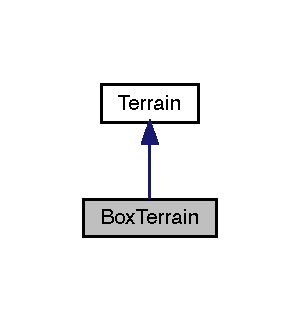
\includegraphics[width=144pt]{class_box_terrain__inherit__graph}
\end{center}
\end{figure}


Collaboration diagram for Box\+Terrain\+:\nopagebreak
\begin{figure}[H]
\begin{center}
\leavevmode
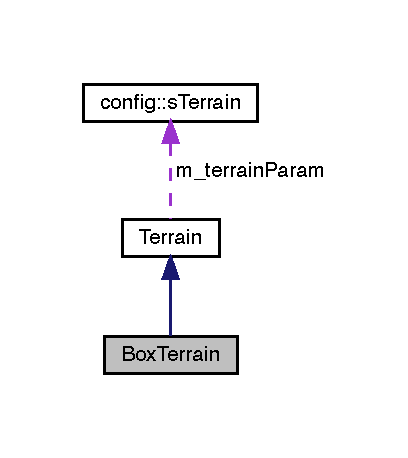
\includegraphics[width=196pt]{class_box_terrain__coll__graph}
\end{center}
\end{figure}
\subsection*{Public Member Functions}
\begin{DoxyCompactItemize}
\item 
\mbox{\Hypertarget{class_box_terrain_a72f481873e9505c75a1702bd61eac8bf}\label{class_box_terrain_a72f481873e9505c75a1702bd61eac8bf}} 
{\bfseries Box\+Terrain} (b2\+World $\ast$world, sf\+::\+Render\+Window \&window, \mbox{\hyperlink{structconfig_1_1s_terrain}{config\+::s\+Terrain}} terrain\+Param, int W\+I\+N\+D\+O\+W\+\_\+\+X\+\_\+\+PX, double body\+Length=1)
\item 
void \mbox{\hyperlink{class_box_terrain_a175fb845b46ed36cd0b4516b4bb64fb3}{create}} (b2\+World $\ast$world, sf\+::\+Render\+Window \&window, \mbox{\hyperlink{structconfig_1_1s_terrain}{config\+::s\+Terrain}} terrain\+Param, int W\+I\+N\+D\+O\+W\+\_\+\+X\+\_\+\+PX, double body\+Length=1)
\item 
void \mbox{\hyperlink{class_box_terrain_a7f5172beaa4e5dcb4d45f3c5e46e3155}{create\+Body}} (b2\+World $\ast$world)
\item 
void \mbox{\hyperlink{class_box_terrain_a309e67722a008ef166198d36add1690a}{draw\+Body}} (sf\+::\+Render\+Window \&window)
\item 
\mbox{\hyperlink{_terrain_8h_a6d0b7e83bb7325270c1162bece970fd8}{e\+\_\+terrain\+\_\+type}} \mbox{\hyperlink{class_box_terrain_a8056b743b0cc1fbd38e742f542dfa34b}{get\+Type}} ()
\end{DoxyCompactItemize}
\subsection*{Additional Inherited Members}


\subsection{Member Function Documentation}
\mbox{\Hypertarget{class_box_terrain_a175fb845b46ed36cd0b4516b4bb64fb3}\label{class_box_terrain_a175fb845b46ed36cd0b4516b4bb64fb3}} 
\index{Box\+Terrain@{Box\+Terrain}!create@{create}}
\index{create@{create}!Box\+Terrain@{Box\+Terrain}}
\subsubsection{\texorpdfstring{create()}{create()}}
{\footnotesize\ttfamily void Box\+Terrain\+::create (\begin{DoxyParamCaption}\item[{b2\+World $\ast$}]{world,  }\item[{sf\+::\+Render\+Window \&}]{window,  }\item[{\mbox{\hyperlink{structconfig_1_1s_terrain}{config\+::s\+Terrain}}}]{terrain\+Param,  }\item[{int}]{W\+I\+N\+D\+O\+W\+\_\+\+X\+\_\+\+PX,  }\item[{double}]{body\+Length = {\ttfamily 1} }\end{DoxyParamCaption})\hspace{0.3cm}{\ttfamily [virtual]}}

The function create M\+U\+ST be called if the terrain object has been created via the default constructor (ex when created dynamically with new), otherwise no need to use it 
\begin{DoxyParams}{Parameters}
{\em world} & is a pointer on the Box2D world object \\
\hline
{\em window} & is the S\+F\+ML window \\
\hline
{\em terrain\+Param} & are the terrain parameters (cf \mbox{\hyperlink{_config_8h_source}{Config.\+h}}) \\
\hline
{\em W\+I\+N\+D\+O\+W\+\_\+\+X\+\_\+\+PX} & is the x-\/size of the window. it is used to calculate the scale to convert from meters to pixels \\
\hline
{\em bodylength} & is the size of a robot. it is used to convert the dimension from body length to m \\
\hline
\end{DoxyParams}


Reimplemented from \mbox{\hyperlink{class_terrain_ae7515dee9afa3b1cefac459abefb5442}{Terrain}}.

Here is the call graph for this function\+:\nopagebreak
\begin{figure}[H]
\begin{center}
\leavevmode
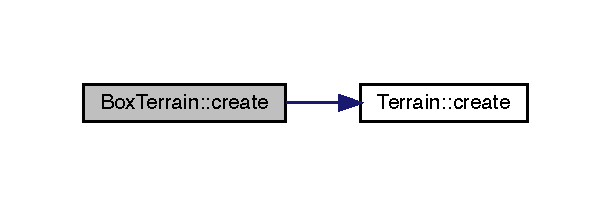
\includegraphics[width=293pt]{class_box_terrain_a175fb845b46ed36cd0b4516b4bb64fb3_cgraph}
\end{center}
\end{figure}
Here is the caller graph for this function\+:\nopagebreak
\begin{figure}[H]
\begin{center}
\leavevmode
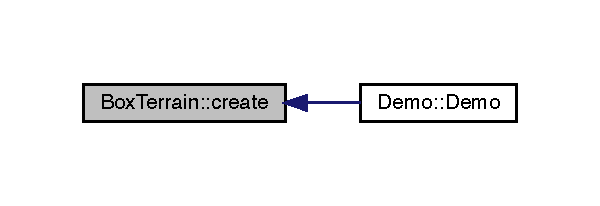
\includegraphics[width=288pt]{class_box_terrain_a175fb845b46ed36cd0b4516b4bb64fb3_icgraph}
\end{center}
\end{figure}
\mbox{\Hypertarget{class_box_terrain_a7f5172beaa4e5dcb4d45f3c5e46e3155}\label{class_box_terrain_a7f5172beaa4e5dcb4d45f3c5e46e3155}} 
\index{Box\+Terrain@{Box\+Terrain}!create\+Body@{create\+Body}}
\index{create\+Body@{create\+Body}!Box\+Terrain@{Box\+Terrain}}
\subsubsection{\texorpdfstring{create\+Body()}{createBody()}}
{\footnotesize\ttfamily void Box\+Terrain\+::create\+Body (\begin{DoxyParamCaption}\item[{b2\+World $\ast$}]{world }\end{DoxyParamCaption})\hspace{0.3cm}{\ttfamily [virtual]}}

Create the Box2D body for the static object of the scene. 
\begin{DoxyParams}{Parameters}
{\em m\+\_\+to\+\_\+pix,window\+\_\+x\+\_\+px,window\+\_\+y\+\_\+px} & configuration of the window, they are usually defined in the config file. \\
\hline
{\em wall\+\_\+w\+\_\+m,wall\+\_\+h\+\_\+m} & configuration of the walls, they are usually defined in the config file. \\
\hline
\end{DoxyParams}


Reimplemented from \mbox{\hyperlink{class_terrain_a97e007277f8abb9dde20ef2b49c38a3a}{Terrain}}.

Here is the caller graph for this function\+:\nopagebreak
\begin{figure}[H]
\begin{center}
\leavevmode
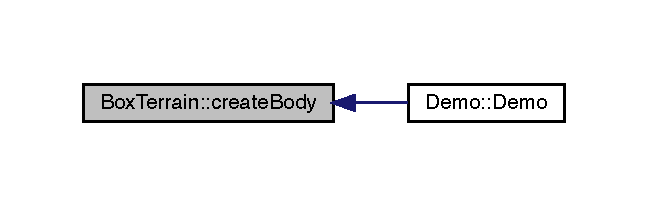
\includegraphics[width=311pt]{class_box_terrain_a7f5172beaa4e5dcb4d45f3c5e46e3155_icgraph}
\end{center}
\end{figure}
\mbox{\Hypertarget{class_box_terrain_a309e67722a008ef166198d36add1690a}\label{class_box_terrain_a309e67722a008ef166198d36add1690a}} 
\index{Box\+Terrain@{Box\+Terrain}!draw\+Body@{draw\+Body}}
\index{draw\+Body@{draw\+Body}!Box\+Terrain@{Box\+Terrain}}
\subsubsection{\texorpdfstring{draw\+Body()}{drawBody()}}
{\footnotesize\ttfamily void Box\+Terrain\+::draw\+Body (\begin{DoxyParamCaption}\item[{sf\+::\+Render\+Window \&}]{window }\end{DoxyParamCaption})\hspace{0.3cm}{\ttfamily [virtual]}}

Draw the shapes corresponding to the Box2D body created previously. 
\begin{DoxyParams}{Parameters}
{\em m\+\_\+to\+\_\+pix,window\+\_\+x\+\_\+px,window\+\_\+y\+\_\+px} & configuration of the window, they are usually defined in the config file. \\
\hline
{\em wall\+\_\+w\+\_\+m,wall\+\_\+h\+\_\+m} & configuration of the walls, they are usually defined in the config file. \\
\hline
\end{DoxyParams}


Reimplemented from \mbox{\hyperlink{class_terrain_ae60571b91c1979fa94bdfc5002da6ac7}{Terrain}}.

Here is the caller graph for this function\+:\nopagebreak
\begin{figure}[H]
\begin{center}
\leavevmode
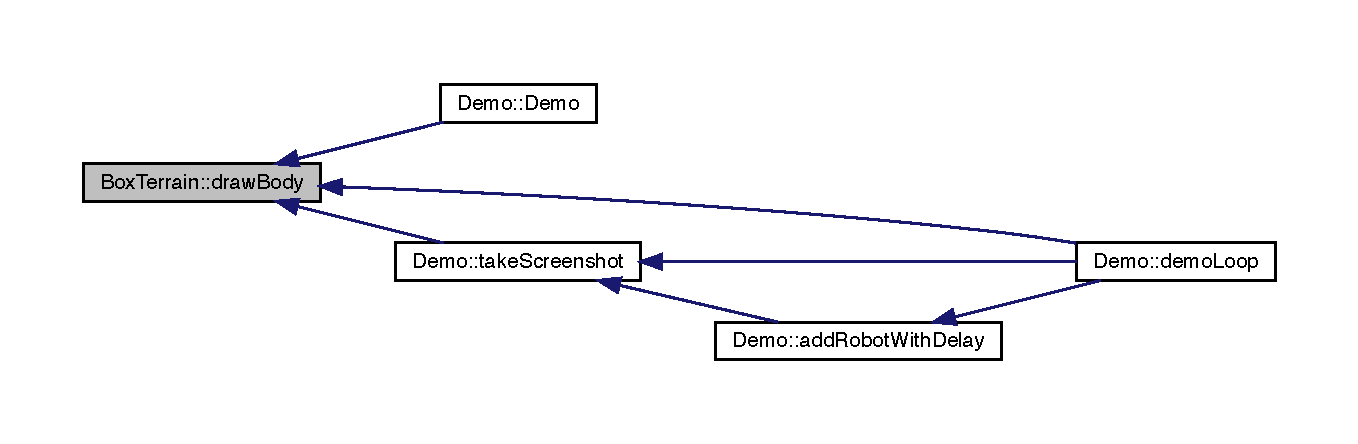
\includegraphics[width=350pt]{class_box_terrain_a309e67722a008ef166198d36add1690a_icgraph}
\end{center}
\end{figure}
\mbox{\Hypertarget{class_box_terrain_a8056b743b0cc1fbd38e742f542dfa34b}\label{class_box_terrain_a8056b743b0cc1fbd38e742f542dfa34b}} 
\index{Box\+Terrain@{Box\+Terrain}!get\+Type@{get\+Type}}
\index{get\+Type@{get\+Type}!Box\+Terrain@{Box\+Terrain}}
\subsubsection{\texorpdfstring{get\+Type()}{getType()}}
{\footnotesize\ttfamily \mbox{\hyperlink{_terrain_8h_a6d0b7e83bb7325270c1162bece970fd8}{e\+\_\+terrain\+\_\+type}} Box\+Terrain\+::get\+Type (\begin{DoxyParamCaption}{ }\end{DoxyParamCaption})\hspace{0.3cm}{\ttfamily [virtual]}}

\begin{DoxyReturn}{Returns}
the type of the terrain. Can be D\+E\+F\+A\+U\+LT, V\+\_\+\+T\+E\+R\+R\+A\+IN, V2\+B\+L\+\_\+\+T\+E\+R\+R\+A\+IN, R\+A\+MP, B\+OX or V\+\_\+\+S\+T\+E\+P\+P\+ER 
\end{DoxyReturn}


Reimplemented from \mbox{\hyperlink{class_terrain_a6cd1220b8e64466cc7a2219efff4141b}{Terrain}}.

Here is the caller graph for this function\+:\nopagebreak
\begin{figure}[H]
\begin{center}
\leavevmode
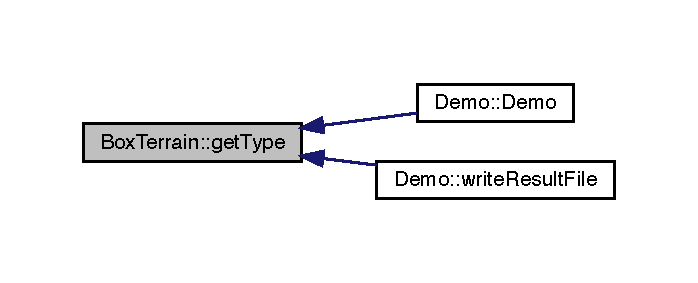
\includegraphics[width=335pt]{class_box_terrain_a8056b743b0cc1fbd38e742f542dfa34b_icgraph}
\end{center}
\end{figure}


The documentation for this class was generated from the following files\+:\begin{DoxyCompactItemize}
\item 
simulation/src/Box\+Terrain.\+h\item 
simulation/src/Box\+Terrain.\+cpp\end{DoxyCompactItemize}

\hypertarget{classconfig_1_1_configuration}{}\section{config\+:\+:Configuration Class Reference}
\label{classconfig_1_1_configuration}\index{config\+::\+Configuration@{config\+::\+Configuration}}
\subsection*{Public Member Functions}
\begin{DoxyCompactItemize}
\item 
\mbox{\Hypertarget{classconfig_1_1_configuration_a793f44d0706db6e3ce92bc024f772869}\label{classconfig_1_1_configuration_a793f44d0706db6e3ce92bc024f772869}} 
void {\bfseries Clear} ()
\item 
\mbox{\Hypertarget{classconfig_1_1_configuration_ac259be785f0656ead250ae257e95b0e3}\label{classconfig_1_1_configuration_ac259be785f0656ead250ae257e95b0e3}} 
bool {\bfseries Load} (const std\+::string \&File)
\item 
\mbox{\Hypertarget{classconfig_1_1_configuration_a51219b5a99dba44cc476d2910a2eec35}\label{classconfig_1_1_configuration_a51219b5a99dba44cc476d2910a2eec35}} 
bool {\bfseries Contains} (const std\+::string \&key) const
\item 
\mbox{\Hypertarget{classconfig_1_1_configuration_a736adaece5e94d67416a752607c59698}\label{classconfig_1_1_configuration_a736adaece5e94d67416a752607c59698}} 
bool {\bfseries Get} (const std\+::string \&key, std\+::string \&value) const
\item 
\mbox{\Hypertarget{classconfig_1_1_configuration_a34d6fdbec3fd5303aa27583c9c0deaba}\label{classconfig_1_1_configuration_a34d6fdbec3fd5303aa27583c9c0deaba}} 
bool {\bfseries Get} (const std\+::string \&key, int \&value) const
\item 
\mbox{\Hypertarget{classconfig_1_1_configuration_a0489785801f516f664f7a2609e1e69a1}\label{classconfig_1_1_configuration_a0489785801f516f664f7a2609e1e69a1}} 
bool {\bfseries Get} (const std\+::string \&key, long \&value) const
\item 
\mbox{\Hypertarget{classconfig_1_1_configuration_a7e1227efb413e823ab80384987076ffb}\label{classconfig_1_1_configuration_a7e1227efb413e823ab80384987076ffb}} 
bool {\bfseries Get} (const std\+::string \&key, double \&value) const
\item 
\mbox{\Hypertarget{classconfig_1_1_configuration_addb88e4bc970862d58700bb16264662d}\label{classconfig_1_1_configuration_addb88e4bc970862d58700bb16264662d}} 
bool {\bfseries Get} (const std\+::string \&key, bool \&value) const
\end{DoxyCompactItemize}


The documentation for this class was generated from the following files\+:\begin{DoxyCompactItemize}
\item 
simulation/src/Config.\+h\item 
simulation/src/Config.\+cpp\end{DoxyCompactItemize}

\hypertarget{class_demo}{}\section{Demo Class Reference}
\label{class_demo}\index{Demo@{Demo}}


{\ttfamily \#include $<$Demo.\+h$>$}

\subsection*{Public Member Functions}
\begin{DoxyCompactItemize}
\item 
\mbox{\hyperlink{class_demo_a7fa722430ba973c538ae230e407854ab}{Demo}} (b2\+World $\ast$m\+\_\+world, \mbox{\hyperlink{structconfig_1_1s_config}{config\+::s\+Config}} cfg)
\item 
bool \mbox{\hyperlink{class_demo_a4636f708574c6be85334ff16373e2292}{add\+Robot\+With\+Delay}} ()
\item 
bool \mbox{\hyperlink{class_demo_a37b03d288a1bf67f586cdfe1f9ba16af}{add\+Robot\+With\+Distance}} ()
\item 
void \mbox{\hyperlink{class_demo_ae0f7fe82aa44b946c13823d408b9ee01}{create\+Bridge\+File}} ()
\item 
void \mbox{\hyperlink{class_demo_a938c3b6ab1c98ce43f977dda9d4f2b3a}{demo\+Loop}} ()
\item 
double \mbox{\hyperlink{class_demo_ac6657b0f7f55a81ba215811d31d9e5b5}{get\+Bridge\+Height}} ()
\item 
\mbox{\hyperlink{class_robot_controller}{Robot\+Controller}} \mbox{\hyperlink{class_demo_af3f1105a11288fd13d54e85ef2485da5}{get\+Controller}} ()
\item 
double \mbox{\hyperlink{class_demo_acd4e28d1626c6979bbab2e396b717cba}{get\+New\+Path\+Length}} ()
\item 
sf\+::\+Render\+Window $\ast$ \mbox{\hyperlink{class_demo_a2b9c1e5275d36c3d82c0d4ee5d8a9741}{get\+Window}} ()
\item 
void \mbox{\hyperlink{class_demo_a585ce54e47b0624ca078492d9aa1c59c}{init}} ()
\item 
void \mbox{\hyperlink{class_demo_a8f833d4d73ccdb28cd2e4387fc3bb9e1}{take\+Screenshot}} (bool draw, int step)
\item 
void \mbox{\hyperlink{class_demo_a1b09c62228a007c49ddc0639a65341b2}{write\+Result\+File}} ()
\item 
void \mbox{\hyperlink{class_demo_a653b6b835b58959fea0758f2a1695002}{write\+Bridge\+File}} ()
\end{DoxyCompactItemize}
\subsection*{Protected Attributes}
\begin{DoxyCompactItemize}
\item 
\mbox{\Hypertarget{class_demo_ab996202da88e954f84e9ce3a9d467065}\label{class_demo_ab996202da88e954f84e9ce3a9d467065}} 
b2\+World $\ast$ {\bfseries m\+\_\+world} = nullptr
\end{DoxyCompactItemize}


\subsection{Detailed Description}
The \mbox{\hyperlink{class_demo}{Demo}} class gather all the elements of the simulation\+: the terrain, the robot controller and the robots and implement more abstract simulation methods. Those methods handle the robot interaction with the terrain and between themselves ie the group behavior. This is why the robots are only created via the robot controller. It also handle the simulation results by writing them in two distinct files\+:
\begin{DoxyItemize}
\item The overall result file with the summary of the results
\item The bridge file that gather the timestep and position of every robots entering the bridge state. It is updated every time a new robot enter the bridge state. 
\end{DoxyItemize}

\subsection{Constructor \& Destructor Documentation}
\mbox{\Hypertarget{class_demo_a7fa722430ba973c538ae230e407854ab}\label{class_demo_a7fa722430ba973c538ae230e407854ab}} 
\index{Demo@{Demo}!Demo@{Demo}}
\index{Demo@{Demo}!Demo@{Demo}}
\subsubsection{\texorpdfstring{Demo()}{Demo()}}
{\footnotesize\ttfamily Demo\+::\+Demo (\begin{DoxyParamCaption}\item[{b2\+World $\ast$}]{m\+\_\+world,  }\item[{\mbox{\hyperlink{structconfig_1_1s_config}{config\+::s\+Config}}}]{cfg }\end{DoxyParamCaption})}

Initial x position of the robot in the world

Initial y position of the robot Here is the call graph for this function\+:\nopagebreak
\begin{figure}[H]
\begin{center}
\leavevmode
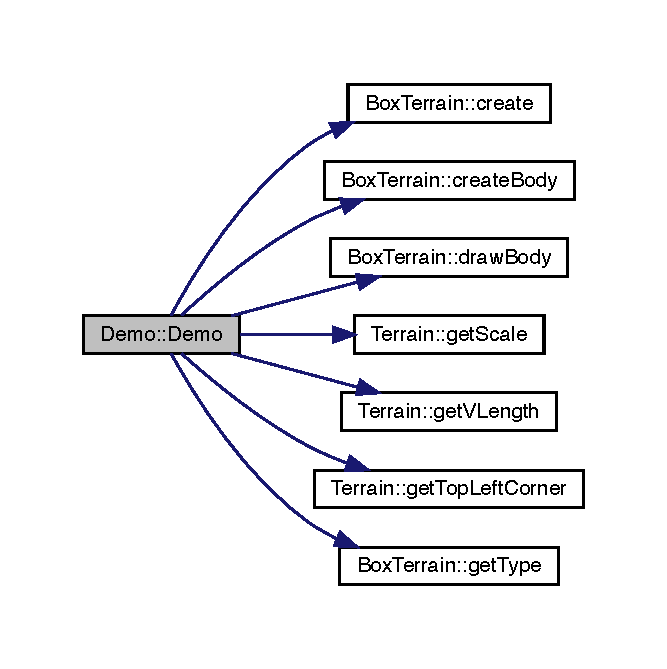
\includegraphics[width=320pt]{class_demo_a7fa722430ba973c538ae230e407854ab_cgraph}
\end{center}
\end{figure}


\subsection{Member Function Documentation}
\mbox{\Hypertarget{class_demo_a4636f708574c6be85334ff16373e2292}\label{class_demo_a4636f708574c6be85334ff16373e2292}} 
\index{Demo@{Demo}!add\+Robot\+With\+Delay@{add\+Robot\+With\+Delay}}
\index{add\+Robot\+With\+Delay@{add\+Robot\+With\+Delay}!Demo@{Demo}}
\subsubsection{\texorpdfstring{add\+Robot\+With\+Delay()}{addRobotWithDelay()}}
{\footnotesize\ttfamily bool Demo\+::add\+Robot\+With\+Delay (\begin{DoxyParamCaption}{ }\end{DoxyParamCaption})}

Create a new robot after a given delay defined by m\+\_\+config.\+simulation.\+robot\+\_\+delay (which has been obtained as an argument of the \mbox{\hyperlink{class_demo}{Demo}} object creation) until the maximum number of robots have been reached. The traffic is thus controlled by the initial position and the delay between the robots. \begin{DoxyReturn}{Returns}
false if the robots are stacking (the previous robot too close to the one that will be created) 
\end{DoxyReturn}
Here is the call graph for this function\+:\nopagebreak
\begin{figure}[H]
\begin{center}
\leavevmode
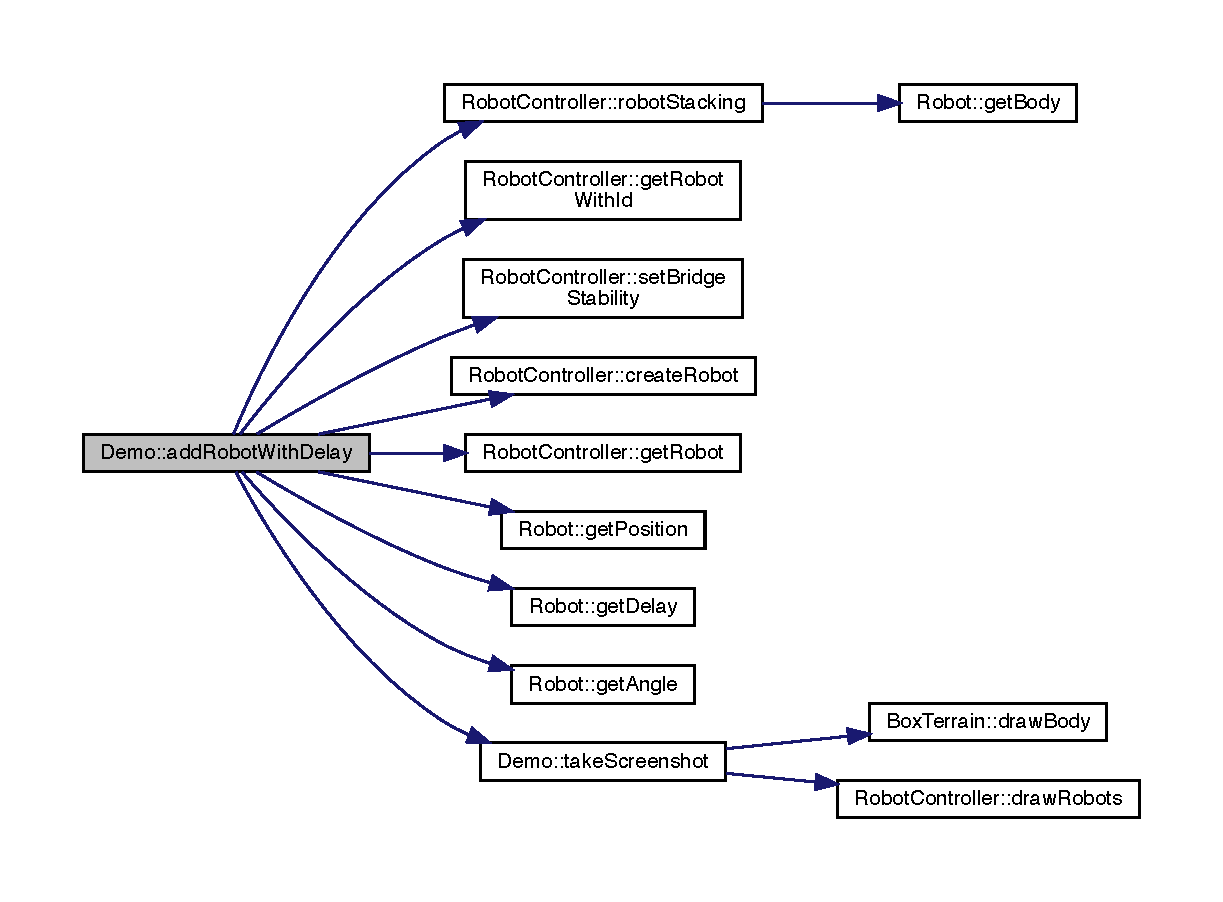
\includegraphics[width=350pt]{class_demo_a4636f708574c6be85334ff16373e2292_cgraph}
\end{center}
\end{figure}
Here is the caller graph for this function\+:\nopagebreak
\begin{figure}[H]
\begin{center}
\leavevmode
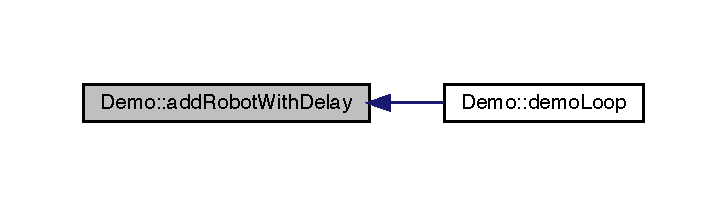
\includegraphics[width=349pt]{class_demo_a4636f708574c6be85334ff16373e2292_icgraph}
\end{center}
\end{figure}
\mbox{\Hypertarget{class_demo_a37b03d288a1bf67f586cdfe1f9ba16af}\label{class_demo_a37b03d288a1bf67f586cdfe1f9ba16af}} 
\index{Demo@{Demo}!add\+Robot\+With\+Distance@{add\+Robot\+With\+Distance}}
\index{add\+Robot\+With\+Distance@{add\+Robot\+With\+Distance}!Demo@{Demo}}
\subsubsection{\texorpdfstring{add\+Robot\+With\+Distance()}{addRobotWithDistance()}}
{\footnotesize\ttfamily bool Demo\+::add\+Robot\+With\+Distance (\begin{DoxyParamCaption}{ }\end{DoxyParamCaption})}

Create a new robot when a given distance with the previous robot defined by m\+\_\+config.\+simulation.\+robot\+\_\+distance has been reached and the previous robot has an angle corresponding to the desired phase shift. It does so until the maximum number of robots have been reached. The traffic is thus controlled by the distance between the robots and the phase shift. \begin{DoxyReturn}{Returns}
true when a new robot is created. 
\end{DoxyReturn}
Here is the call graph for this function\+:\nopagebreak
\begin{figure}[H]
\begin{center}
\leavevmode
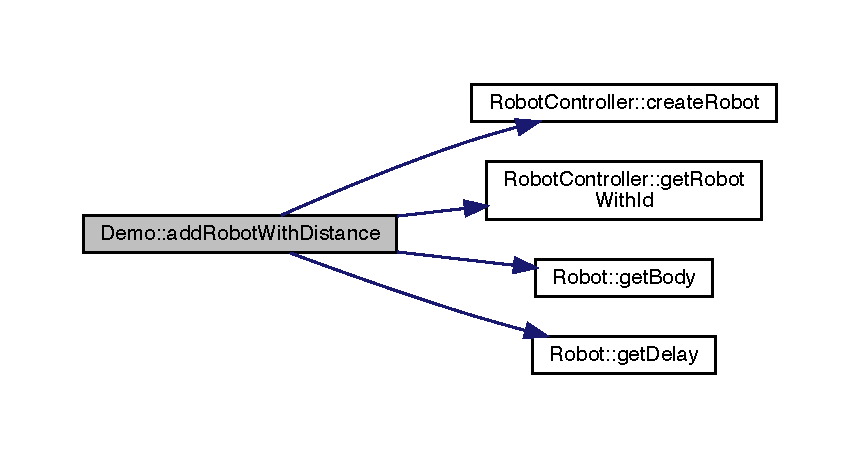
\includegraphics[width=350pt]{class_demo_a37b03d288a1bf67f586cdfe1f9ba16af_cgraph}
\end{center}
\end{figure}
\mbox{\Hypertarget{class_demo_ae0f7fe82aa44b946c13823d408b9ee01}\label{class_demo_ae0f7fe82aa44b946c13823d408b9ee01}} 
\index{Demo@{Demo}!create\+Bridge\+File@{create\+Bridge\+File}}
\index{create\+Bridge\+File@{create\+Bridge\+File}!Demo@{Demo}}
\subsubsection{\texorpdfstring{create\+Bridge\+File()}{createBridgeFile()}}
{\footnotesize\ttfamily void Demo\+::create\+Bridge\+File (\begin{DoxyParamCaption}{ }\end{DoxyParamCaption})}

Create bridge file under m\+\_\+bridge\+File. Every line is structured as follow\+: Timestamp; robot ID; x coordinate; y coordinate; angle; current joint x; current joint y; previous joint x; previous joint y; it entry; age Here is the caller graph for this function\+:\nopagebreak
\begin{figure}[H]
\begin{center}
\leavevmode
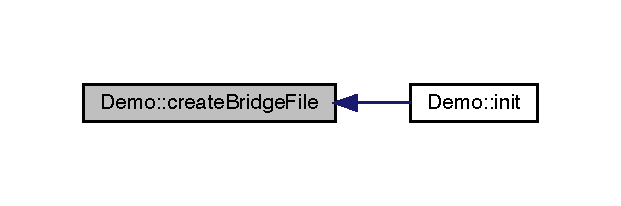
\includegraphics[width=298pt]{class_demo_ae0f7fe82aa44b946c13823d408b9ee01_icgraph}
\end{center}
\end{figure}
\mbox{\Hypertarget{class_demo_a938c3b6ab1c98ce43f977dda9d4f2b3a}\label{class_demo_a938c3b6ab1c98ce43f977dda9d4f2b3a}} 
\index{Demo@{Demo}!demo\+Loop@{demo\+Loop}}
\index{demo\+Loop@{demo\+Loop}!Demo@{Demo}}
\subsubsection{\texorpdfstring{demo\+Loop()}{demoLoop()}}
{\footnotesize\ttfamily Both cases are then almost identical apart from the simulation part void Demo\+::demo\+Loop (\begin{DoxyParamCaption}{ }\end{DoxyParamCaption})}

Simulation loop that handle the synchronization between the physics and the controller step. The visualization is activated or deactivated via m\+\_\+config.\+simulation.\+visualization. The Simulation is composed of two steps\+: the bridge formation where new robots are created following the given delay or distance and the bridge dissolution step where no more robots are created. The duration of the two steps are determined by respectively m\+\_\+config.\+simulation.\+bridge\+\_\+duration and m\+\_\+config.\+simulation.\+dissolution\+\_\+duration. The results are written in the two distinct files. Data processing Precise the simulation parameters\+: distance between robots, speed Get time of the first bridge contact get time when the last robot enter the stable bridge state get points of contact for every robot + position and orientation of centerHere is the call graph for this function\+:\nopagebreak
\begin{figure}[H]
\begin{center}
\leavevmode
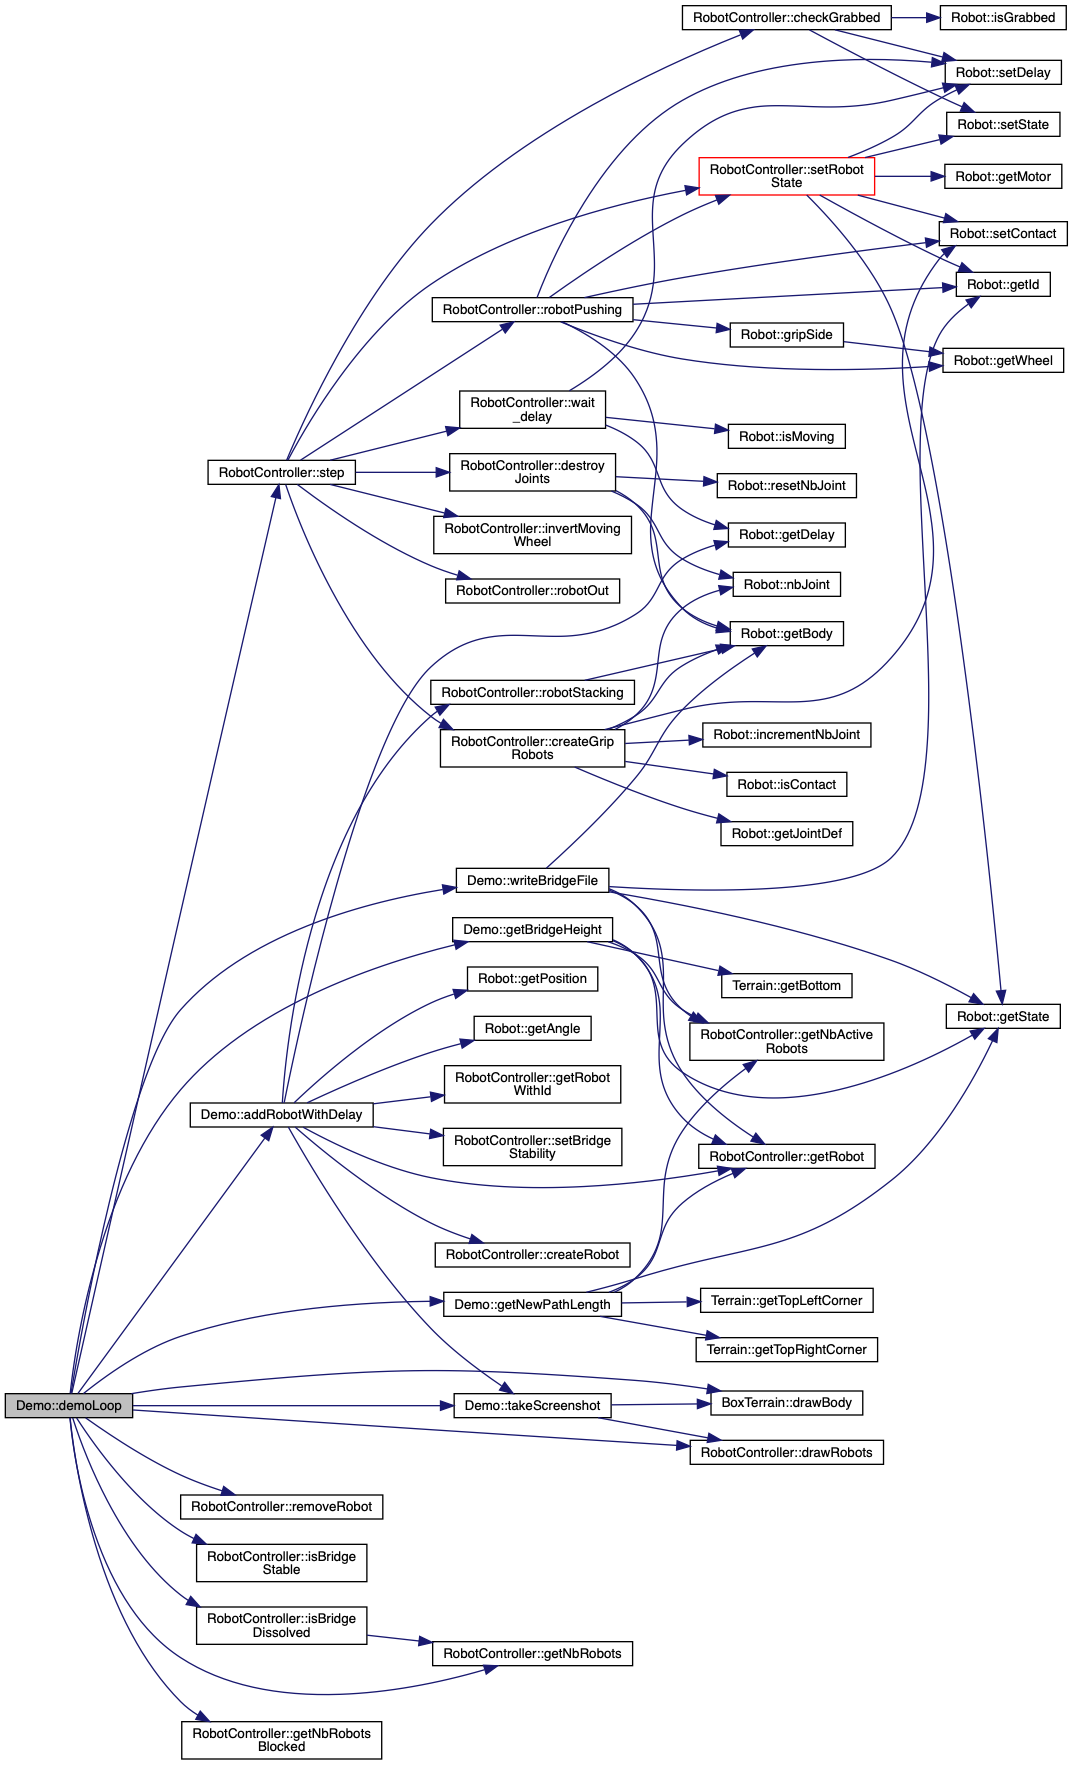
\includegraphics[width=350pt]{class_demo_a938c3b6ab1c98ce43f977dda9d4f2b3a_cgraph}
\end{center}
\end{figure}
\mbox{\Hypertarget{class_demo_ac6657b0f7f55a81ba215811d31d9e5b5}\label{class_demo_ac6657b0f7f55a81ba215811d31d9e5b5}} 
\index{Demo@{Demo}!get\+Bridge\+Height@{get\+Bridge\+Height}}
\index{get\+Bridge\+Height@{get\+Bridge\+Height}!Demo@{Demo}}
\subsubsection{\texorpdfstring{get\+Bridge\+Height()}{getBridgeHeight()}}
{\footnotesize\ttfamily double Demo\+::get\+Bridge\+Height (\begin{DoxyParamCaption}{ }\end{DoxyParamCaption})}

Get the bridge height. This function is not up to date and should not be used in this state Here is the call graph for this function\+:\nopagebreak
\begin{figure}[H]
\begin{center}
\leavevmode
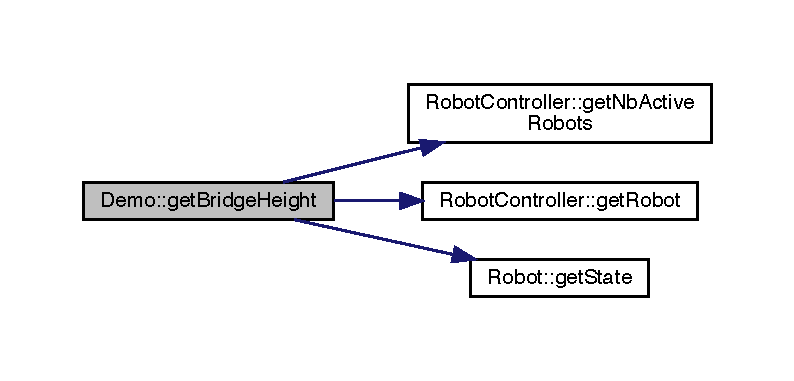
\includegraphics[width=350pt]{class_demo_ac6657b0f7f55a81ba215811d31d9e5b5_cgraph}
\end{center}
\end{figure}
\mbox{\Hypertarget{class_demo_af3f1105a11288fd13d54e85ef2485da5}\label{class_demo_af3f1105a11288fd13d54e85ef2485da5}} 
\index{Demo@{Demo}!get\+Controller@{get\+Controller}}
\index{get\+Controller@{get\+Controller}!Demo@{Demo}}
\subsubsection{\texorpdfstring{get\+Controller()}{getController()}}
{\footnotesize\ttfamily \mbox{\hyperlink{class_robot_controller}{Robot\+Controller}} Demo\+::get\+Controller (\begin{DoxyParamCaption}{ }\end{DoxyParamCaption})}

Get the robot controller object Rq\+: in future development, could be adapted to be a pointer \begin{DoxyReturn}{Returns}
the robot controller object 
\end{DoxyReturn}
\mbox{\Hypertarget{class_demo_acd4e28d1626c6979bbab2e396b717cba}\label{class_demo_acd4e28d1626c6979bbab2e396b717cba}} 
\index{Demo@{Demo}!get\+New\+Path\+Length@{get\+New\+Path\+Length}}
\index{get\+New\+Path\+Length@{get\+New\+Path\+Length}!Demo@{Demo}}
\subsubsection{\texorpdfstring{get\+New\+Path\+Length()}{getNewPathLength()}}
{\footnotesize\ttfamily double Demo\+::get\+New\+Path\+Length (\begin{DoxyParamCaption}{ }\end{DoxyParamCaption})}

Get the new path length induced by the bridge from the left corner of the obstacle to its right corner. This function is not up to date and should not be used in this state. Here is the call graph for this function\+:\nopagebreak
\begin{figure}[H]
\begin{center}
\leavevmode
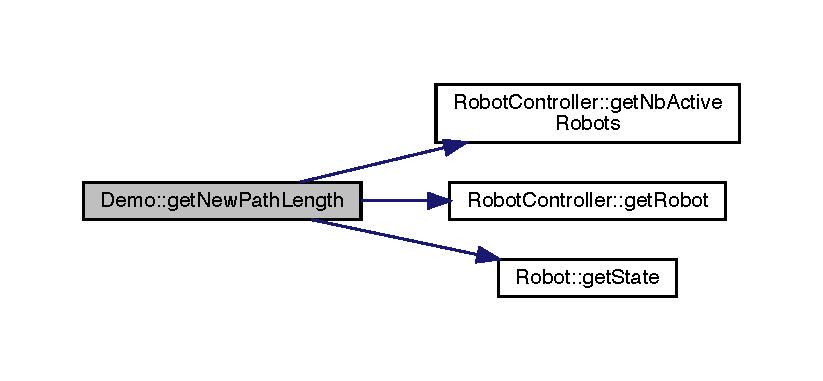
\includegraphics[width=350pt]{class_demo_acd4e28d1626c6979bbab2e396b717cba_cgraph}
\end{center}
\end{figure}
\mbox{\Hypertarget{class_demo_a2b9c1e5275d36c3d82c0d4ee5d8a9741}\label{class_demo_a2b9c1e5275d36c3d82c0d4ee5d8a9741}} 
\index{Demo@{Demo}!get\+Window@{get\+Window}}
\index{get\+Window@{get\+Window}!Demo@{Demo}}
\subsubsection{\texorpdfstring{get\+Window()}{getWindow()}}
{\footnotesize\ttfamily sf\+::\+Render\+Window $\ast$ Demo\+::get\+Window (\begin{DoxyParamCaption}{ }\end{DoxyParamCaption})}

Get a pointer on the S\+F\+ML window \begin{DoxyReturn}{Returns}
a pointer on the S\+F\+ML window 
\end{DoxyReturn}
\mbox{\Hypertarget{class_demo_a585ce54e47b0624ca078492d9aa1c59c}\label{class_demo_a585ce54e47b0624ca078492d9aa1c59c}} 
\index{Demo@{Demo}!init@{init}}
\index{init@{init}!Demo@{Demo}}
\subsubsection{\texorpdfstring{init()}{init()}}
{\footnotesize\ttfamily void Demo\+::init (\begin{DoxyParamCaption}{ }\end{DoxyParamCaption})}

Initialize the demo Here is the call graph for this function\+:\nopagebreak
\begin{figure}[H]
\begin{center}
\leavevmode
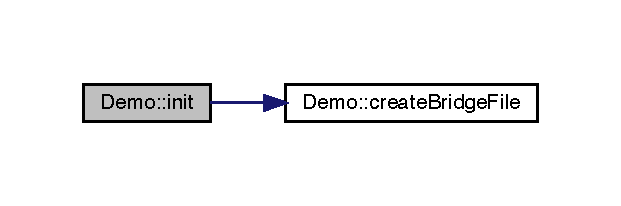
\includegraphics[width=298pt]{class_demo_a585ce54e47b0624ca078492d9aa1c59c_cgraph}
\end{center}
\end{figure}
\mbox{\Hypertarget{class_demo_a8f833d4d73ccdb28cd2e4387fc3bb9e1}\label{class_demo_a8f833d4d73ccdb28cd2e4387fc3bb9e1}} 
\index{Demo@{Demo}!take\+Screenshot@{take\+Screenshot}}
\index{take\+Screenshot@{take\+Screenshot}!Demo@{Demo}}
\subsubsection{\texorpdfstring{take\+Screenshot()}{takeScreenshot()}}
{\footnotesize\ttfamily void Demo\+::take\+Screenshot (\begin{DoxyParamCaption}\item[{bool}]{draw,  }\item[{int}]{step }\end{DoxyParamCaption})}

Take a screenshot of the simulation at a given time step. The image is saved under m\+\_\+config.\+logfile\+\_\+path + m\+\_\+config.\+logfile\+\_\+name + \char`\"{}\+\_\+dissolution\+\_\+\char`\"{} + std\+::to\+\_\+string(m\+\_\+current\+It) + \char`\"{}.\+jpg\char`\"{} 
\begin{DoxyParams}{Parameters}
{\em draw} & should be true if the window has to be drawn beforehand. It is the case when the visualization is deactivated \\
\hline
{\em step} & is the simulation step\+: it is either 1 if the simulation is in the bridge formation step or 2 if the simulation is in the bridge dissolution one. \\
\hline
\end{DoxyParams}
Here is the call graph for this function\+:\nopagebreak
\begin{figure}[H]
\begin{center}
\leavevmode
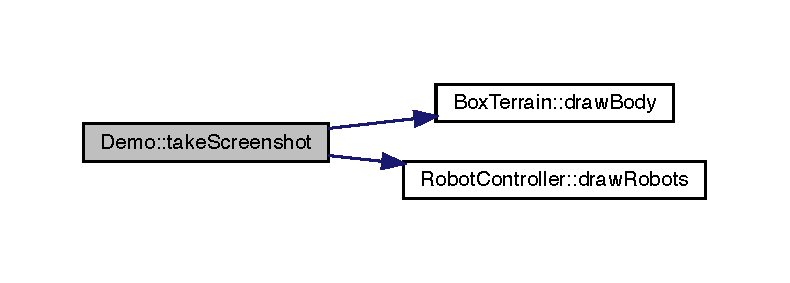
\includegraphics[width=350pt]{class_demo_a8f833d4d73ccdb28cd2e4387fc3bb9e1_cgraph}
\end{center}
\end{figure}
Here is the caller graph for this function\+:\nopagebreak
\begin{figure}[H]
\begin{center}
\leavevmode
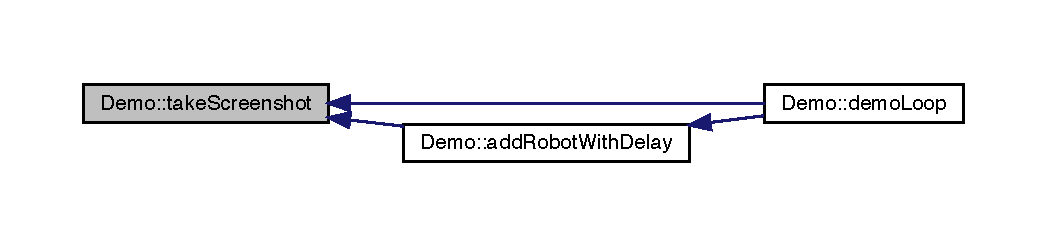
\includegraphics[width=350pt]{class_demo_a8f833d4d73ccdb28cd2e4387fc3bb9e1_icgraph}
\end{center}
\end{figure}
\mbox{\Hypertarget{class_demo_a653b6b835b58959fea0758f2a1695002}\label{class_demo_a653b6b835b58959fea0758f2a1695002}} 
\index{Demo@{Demo}!write\+Bridge\+File@{write\+Bridge\+File}}
\index{write\+Bridge\+File@{write\+Bridge\+File}!Demo@{Demo}}
\subsubsection{\texorpdfstring{write\+Bridge\+File()}{writeBridgeFile()}}
{\footnotesize\ttfamily void Demo\+::write\+Bridge\+File (\begin{DoxyParamCaption}{ }\end{DoxyParamCaption})}

Write the file containing the bridge formation details. This file is updated every time a new robot enter the bridge state The file is saved under m\+\_\+config.\+logfile\+\_\+path + m\+\_\+config.\+logfile\+\_\+name + \char`\"{}\+\_\+bridge.\+txt\char`\"{}; \mbox{\hyperlink{class_robot}{Robot}} id and age

\mbox{\hyperlink{class_robot}{Robot}} position

Joint position Here is the call graph for this function\+:\nopagebreak
\begin{figure}[H]
\begin{center}
\leavevmode
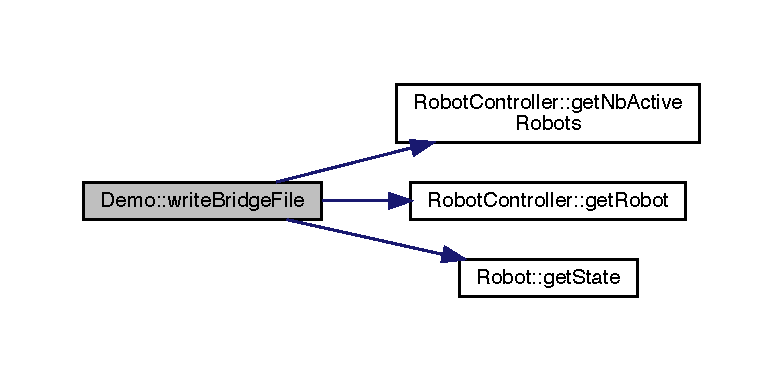
\includegraphics[width=350pt]{class_demo_a653b6b835b58959fea0758f2a1695002_cgraph}
\end{center}
\end{figure}
Here is the caller graph for this function\+:\nopagebreak
\begin{figure}[H]
\begin{center}
\leavevmode
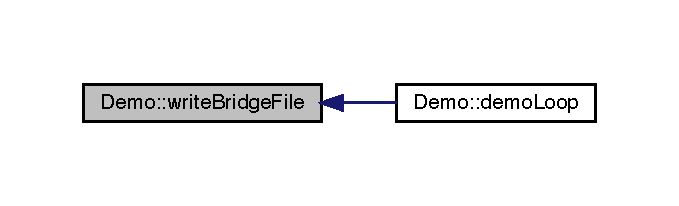
\includegraphics[width=326pt]{class_demo_a653b6b835b58959fea0758f2a1695002_icgraph}
\end{center}
\end{figure}
\mbox{\Hypertarget{class_demo_a1b09c62228a007c49ddc0639a65341b2}\label{class_demo_a1b09c62228a007c49ddc0639a65341b2}} 
\index{Demo@{Demo}!write\+Result\+File@{write\+Result\+File}}
\index{write\+Result\+File@{write\+Result\+File}!Demo@{Demo}}
\subsubsection{\texorpdfstring{write\+Result\+File()}{writeResultFile()}}
{\footnotesize\ttfamily void Demo\+::write\+Result\+File (\begin{DoxyParamCaption}{ }\end{DoxyParamCaption})}

Write the file containing the summary of the simulation results The file is saved under m\+\_\+config.\+logfile\+\_\+path + m\+\_\+config.\+logfile\+\_\+name + \char`\"{}\+\_\+result.\+txt\char`\"{}; \mbox{\hyperlink{class_terrain}{Terrain}} parameters ~\newline
~\newline
~\newline
~\newline
~\newline
 Simulation parameters ~\newline
~\newline
~\newline
~\newline
 Controller parameters ~\newline
~\newline
~\newline
 Controller parameters ~\newline
~\newline
 Bridge parameters ~\newline
 Dissolution parameters Here is the call graph for this function\+:\nopagebreak
\begin{figure}[H]
\begin{center}
\leavevmode
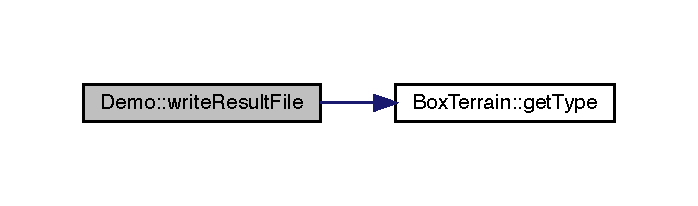
\includegraphics[width=335pt]{class_demo_a1b09c62228a007c49ddc0639a65341b2_cgraph}
\end{center}
\end{figure}


The documentation for this class was generated from the following files\+:\begin{DoxyCompactItemize}
\item 
simulation/src/\mbox{\hyperlink{_demo_8h}{Demo.\+h}}\item 
simulation/src/Demo.\+cpp\end{DoxyCompactItemize}

\hypertarget{class_my_contact_listener__v2}{}\section{My\+Contact\+Listener\+\_\+v2 Class Reference}
\label{class_my_contact_listener__v2}\index{My\+Contact\+Listener\+\_\+v2@{My\+Contact\+Listener\+\_\+v2}}


{\ttfamily \#include $<$Demo.\+h$>$}



Inheritance diagram for My\+Contact\+Listener\+\_\+v2\+:\nopagebreak
\begin{figure}[H]
\begin{center}
\leavevmode
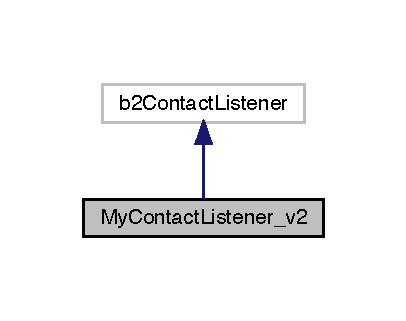
\includegraphics[width=195pt]{class_my_contact_listener__v2__inherit__graph}
\end{center}
\end{figure}


Collaboration diagram for My\+Contact\+Listener\+\_\+v2\+:\nopagebreak
\begin{figure}[H]
\begin{center}
\leavevmode
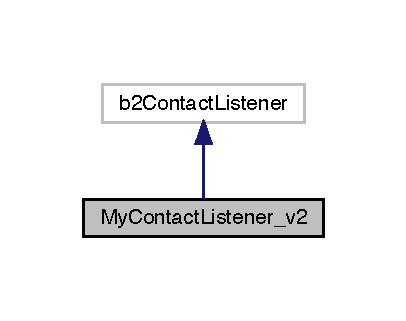
\includegraphics[width=195pt]{class_my_contact_listener__v2__coll__graph}
\end{center}
\end{figure}
\subsection*{Public Member Functions}
\begin{DoxyCompactItemize}
\item 
\mbox{\Hypertarget{class_my_contact_listener__v2_a63de901c8048399d0808d5e37ec6d570}\label{class_my_contact_listener__v2_a63de901c8048399d0808d5e37ec6d570}} 
{\bfseries My\+Contact\+Listener\+\_\+v2} (\mbox{\hyperlink{class_robot_controller}{Robot\+Controller}} \&robot\+Controller)
\item 
\mbox{\Hypertarget{class_my_contact_listener__v2_ac776026bb2a50ca98ab21ca962bb5cf7}\label{class_my_contact_listener__v2_ac776026bb2a50ca98ab21ca962bb5cf7}} 
void {\bfseries Begin\+Contact} (b2\+Contact $\ast$contact)
\item 
\mbox{\Hypertarget{class_my_contact_listener__v2_a23897451bdb6e6505676a6ebb89cde90}\label{class_my_contact_listener__v2_a23897451bdb6e6505676a6ebb89cde90}} 
void {\bfseries End\+Contact} (b2\+Contact $\ast$contact)
\end{DoxyCompactItemize}


\subsection{Detailed Description}
This class is a listener on the box2D body contacts. In case of contact it calls the Robot\+Controller\+::find\+Contact\+Robots(contact) method 

The documentation for this class was generated from the following file\+:\begin{DoxyCompactItemize}
\item 
simulation/src/\mbox{\hyperlink{_demo_8h}{Demo.\+h}}\end{DoxyCompactItemize}

\hypertarget{class_ramp}{}\section{Ramp Class Reference}
\label{class_ramp}\index{Ramp@{Ramp}}


Inheritance diagram for Ramp\+:\nopagebreak
\begin{figure}[H]
\begin{center}
\leavevmode
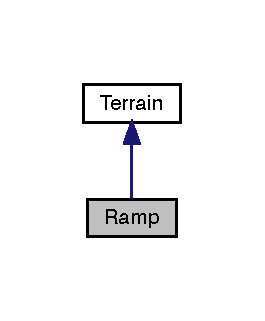
\includegraphics[width=127pt]{class_ramp__inherit__graph}
\end{center}
\end{figure}


Collaboration diagram for Ramp\+:\nopagebreak
\begin{figure}[H]
\begin{center}
\leavevmode
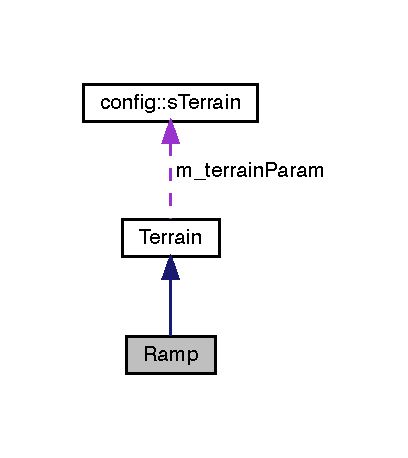
\includegraphics[width=196pt]{class_ramp__coll__graph}
\end{center}
\end{figure}
\subsection*{Public Member Functions}
\begin{DoxyCompactItemize}
\item 
\mbox{\Hypertarget{class_ramp_ad98b8011f89d359a95afe5e390443b03}\label{class_ramp_ad98b8011f89d359a95afe5e390443b03}} 
{\bfseries Ramp} (b2\+World $\ast$world, sf\+::\+Render\+Window \&window, \mbox{\hyperlink{structconfig_1_1s_terrain}{config\+::s\+Terrain}} terrain\+Param, int W\+I\+N\+D\+O\+W\+\_\+\+X\+\_\+\+PX, double body\+Length=1)
\item 
void \mbox{\hyperlink{class_ramp_a0dcb7d44807cb9ce61307c975b29f06e}{create}} (b2\+World $\ast$world, sf\+::\+Render\+Window \&window, \mbox{\hyperlink{structconfig_1_1s_terrain}{config\+::s\+Terrain}} terrain\+Param, int W\+I\+N\+D\+O\+W\+\_\+\+X\+\_\+\+PX, double body\+Length=1)
\item 
void \mbox{\hyperlink{class_ramp_a12049389b07cc2bff4932004c8357dd2}{create\+Body}} (b2\+World $\ast$world)
\item 
void \mbox{\hyperlink{class_ramp_ab05c0a8c5706488be4aba9c4f52f55c9}{draw\+Body}} (sf\+::\+Render\+Window \&window)
\item 
\mbox{\hyperlink{_terrain_8h_a6d0b7e83bb7325270c1162bece970fd8}{e\+\_\+terrain\+\_\+type}} \mbox{\hyperlink{class_ramp_a25dce9bce336a8524be1de1abd6f1af3}{get\+Type}} ()
\item 
b2\+Vec2 \mbox{\hyperlink{class_ramp_aefcb53f7b43d3706400e7f16c77a7e18}{get\+Top\+Left\+Corner}} ()
\item 
b2\+Vec2 \mbox{\hyperlink{class_ramp_a72b5d41278e4ff65df8f80657ae7d9e1}{get\+Top\+Right\+Corner}} ()
\item 
b2\+Vec2 \mbox{\hyperlink{class_ramp_a6e4926a2d16651162340113155e91e8f}{get\+Bottom}} ()
\end{DoxyCompactItemize}
\subsection*{Additional Inherited Members}


\subsection{Member Function Documentation}
\mbox{\Hypertarget{class_ramp_a0dcb7d44807cb9ce61307c975b29f06e}\label{class_ramp_a0dcb7d44807cb9ce61307c975b29f06e}} 
\index{Ramp@{Ramp}!create@{create}}
\index{create@{create}!Ramp@{Ramp}}
\subsubsection{\texorpdfstring{create()}{create()}}
{\footnotesize\ttfamily void Ramp\+::create (\begin{DoxyParamCaption}\item[{b2\+World $\ast$}]{world,  }\item[{sf\+::\+Render\+Window \&}]{window,  }\item[{\mbox{\hyperlink{structconfig_1_1s_terrain}{config\+::s\+Terrain}}}]{terrain\+Param,  }\item[{int}]{W\+I\+N\+D\+O\+W\+\_\+\+X\+\_\+\+PX,  }\item[{double}]{body\+Length = {\ttfamily 1} }\end{DoxyParamCaption})\hspace{0.3cm}{\ttfamily [virtual]}}

The function create M\+U\+ST be called if the terrain object has been created via the default constructor (ex when created dynamically with new), otherwise no need to use it 
\begin{DoxyParams}{Parameters}
{\em world} & is a pointer on the Box2D world object \\
\hline
{\em window} & is the S\+F\+ML window \\
\hline
{\em terrain\+Param} & are the terrain parameters (cf \mbox{\hyperlink{_config_8h}{Config.\+h}}) \\
\hline
{\em W\+I\+N\+D\+O\+W\+\_\+\+X\+\_\+\+PX} & is the x-\/size of the window. it is used to calculate the scale to convert from meters to pixels \\
\hline
{\em bodylength} & is the size of a robot. it is used to convert the dimension from body length to m \\
\hline
\end{DoxyParams}


Reimplemented from \mbox{\hyperlink{class_terrain_ae7515dee9afa3b1cefac459abefb5442}{Terrain}}.

\mbox{\Hypertarget{class_ramp_a12049389b07cc2bff4932004c8357dd2}\label{class_ramp_a12049389b07cc2bff4932004c8357dd2}} 
\index{Ramp@{Ramp}!create\+Body@{create\+Body}}
\index{create\+Body@{create\+Body}!Ramp@{Ramp}}
\subsubsection{\texorpdfstring{create\+Body()}{createBody()}}
{\footnotesize\ttfamily void Ramp\+::create\+Body (\begin{DoxyParamCaption}\item[{b2\+World $\ast$}]{world }\end{DoxyParamCaption})\hspace{0.3cm}{\ttfamily [virtual]}}

Create the Box2D static body of the terrain 
\begin{DoxyParams}{Parameters}
{\em world} & is a pointer on the Box2D world \\
\hline
\end{DoxyParams}


Reimplemented from \mbox{\hyperlink{class_terrain_a97e007277f8abb9dde20ef2b49c38a3a}{Terrain}}.

\mbox{\Hypertarget{class_ramp_ab05c0a8c5706488be4aba9c4f52f55c9}\label{class_ramp_ab05c0a8c5706488be4aba9c4f52f55c9}} 
\index{Ramp@{Ramp}!draw\+Body@{draw\+Body}}
\index{draw\+Body@{draw\+Body}!Ramp@{Ramp}}
\subsubsection{\texorpdfstring{draw\+Body()}{drawBody()}}
{\footnotesize\ttfamily void Ramp\+::draw\+Body (\begin{DoxyParamCaption}\item[{sf\+::\+Render\+Window \&}]{window }\end{DoxyParamCaption})\hspace{0.3cm}{\ttfamily [virtual]}}

Draw the body on the window using the S\+F\+ML library 
\begin{DoxyParams}{Parameters}
{\em window} & is the S\+F\+ML window where the terrain will be drawn \\
\hline
\end{DoxyParams}


Reimplemented from \mbox{\hyperlink{class_terrain_ae60571b91c1979fa94bdfc5002da6ac7}{Terrain}}.

\mbox{\Hypertarget{class_ramp_a6e4926a2d16651162340113155e91e8f}\label{class_ramp_a6e4926a2d16651162340113155e91e8f}} 
\index{Ramp@{Ramp}!get\+Bottom@{get\+Bottom}}
\index{get\+Bottom@{get\+Bottom}!Ramp@{Ramp}}
\subsubsection{\texorpdfstring{get\+Bottom()}{getBottom()}}
{\footnotesize\ttfamily b2\+Vec2 Ramp\+::get\+Bottom (\begin{DoxyParamCaption}{ }\end{DoxyParamCaption})\hspace{0.3cm}{\ttfamily [virtual]}}

\begin{DoxyReturn}{Returns}
the position of the bottom of the V in the box2D world coordinates \mbox{[}m\mbox{]}

the position of bottom of the V in the box2D world coordinates \mbox{[}m\mbox{]} 
\end{DoxyReturn}


Reimplemented from \mbox{\hyperlink{class_terrain_a26e1c7c05b8256015730df34d97d29c2}{Terrain}}.

\mbox{\Hypertarget{class_ramp_aefcb53f7b43d3706400e7f16c77a7e18}\label{class_ramp_aefcb53f7b43d3706400e7f16c77a7e18}} 
\index{Ramp@{Ramp}!get\+Top\+Left\+Corner@{get\+Top\+Left\+Corner}}
\index{get\+Top\+Left\+Corner@{get\+Top\+Left\+Corner}!Ramp@{Ramp}}
\subsubsection{\texorpdfstring{get\+Top\+Left\+Corner()}{getTopLeftCorner()}}
{\footnotesize\ttfamily b2\+Vec2 Ramp\+::get\+Top\+Left\+Corner (\begin{DoxyParamCaption}{ }\end{DoxyParamCaption})\hspace{0.3cm}{\ttfamily [virtual]}}

\begin{DoxyReturn}{Returns}
the position of the Top left corner of the V in the box2D world coordinates \mbox{[}m\mbox{]} 
\end{DoxyReturn}


Reimplemented from \mbox{\hyperlink{class_terrain_a8a8629396e5cb03961649acdc23eacf2}{Terrain}}.

\mbox{\Hypertarget{class_ramp_a72b5d41278e4ff65df8f80657ae7d9e1}\label{class_ramp_a72b5d41278e4ff65df8f80657ae7d9e1}} 
\index{Ramp@{Ramp}!get\+Top\+Right\+Corner@{get\+Top\+Right\+Corner}}
\index{get\+Top\+Right\+Corner@{get\+Top\+Right\+Corner}!Ramp@{Ramp}}
\subsubsection{\texorpdfstring{get\+Top\+Right\+Corner()}{getTopRightCorner()}}
{\footnotesize\ttfamily b2\+Vec2 Ramp\+::get\+Top\+Right\+Corner (\begin{DoxyParamCaption}{ }\end{DoxyParamCaption})\hspace{0.3cm}{\ttfamily [virtual]}}

\begin{DoxyReturn}{Returns}
the position of the Top right corner of the V in the box2D world coordinates \mbox{[}m\mbox{]} 
\end{DoxyReturn}


Reimplemented from \mbox{\hyperlink{class_terrain_a10fcf414cba83e769d99156fe16aa795}{Terrain}}.

\mbox{\Hypertarget{class_ramp_a25dce9bce336a8524be1de1abd6f1af3}\label{class_ramp_a25dce9bce336a8524be1de1abd6f1af3}} 
\index{Ramp@{Ramp}!get\+Type@{get\+Type}}
\index{get\+Type@{get\+Type}!Ramp@{Ramp}}
\subsubsection{\texorpdfstring{get\+Type()}{getType()}}
{\footnotesize\ttfamily \mbox{\hyperlink{_terrain_8h_a6d0b7e83bb7325270c1162bece970fd8}{e\+\_\+terrain\+\_\+type}} Ramp\+::get\+Type (\begin{DoxyParamCaption}{ }\end{DoxyParamCaption})\hspace{0.3cm}{\ttfamily [virtual]}}

return the terrain type, from this class it returns V2\+B\+L\+\_\+\+T\+E\+R\+R\+A\+IN 

Reimplemented from \mbox{\hyperlink{class_terrain_a6cd1220b8e64466cc7a2219efff4141b}{Terrain}}.



The documentation for this class was generated from the following files\+:\begin{DoxyCompactItemize}
\item 
simulation/src/\mbox{\hyperlink{_ramp_8h}{Ramp.\+h}}\item 
simulation/src/Ramp.\+cpp\end{DoxyCompactItemize}

\hypertarget{class_robot}{}\section{Robot Class Reference}
\label{class_robot}\index{Robot@{Robot}}


{\ttfamily \#include $<$Robot.\+h$>$}

\subsection*{Public Member Functions}
\begin{DoxyCompactItemize}
\item 
\mbox{\Hypertarget{class_robot_ac12d142fb87c4985e61f31c3684fe858}\label{class_robot_ac12d142fb87c4985e61f31c3684fe858}} 
{\bfseries Robot} (b2\+World $\ast$world, \mbox{\hyperlink{structconfig_1_1s_robot}{config\+::s\+Robot}} robot\+Parameters, double posX, double posY, double angle=0)
\item 
void \mbox{\hyperlink{class_robot_a7be383b14986610db597c2b26c475cbe}{create\+Body}} (b2\+World $\ast$world, \mbox{\hyperlink{structconfig_1_1s_robot}{config\+::s\+Robot}} m\+\_\+robot\+Parameters, double posX, double posY, double angle=0)
\item 
void \mbox{\hyperlink{class_robot_aae700fce06eb367ff9282492cc17ccc7}{draw\+Body}} (sf\+::\+Render\+Window \&window, double m\+\_\+to\+\_\+pix)
\item 
void \mbox{\hyperlink{class_robot_a94bec26489e5354d1b9106bbd0e59f00}{draw\+Joint}} (sf\+::\+Render\+Window \&window, double m\+\_\+to\+\_\+px)
\item 
void \mbox{\hyperlink{class_robot_a99e6a9dacaae1c43f249a01485352dcf}{draw\+Grip\+Joint}} (sf\+::\+Render\+Window \&window, double m\+\_\+to\+\_\+px)
\item 
void \mbox{\hyperlink{class_robot_a55036d85a36c4e8ed3ff6f8381331c70}{move\+Body\+With\+Motor}} ()
\item 
void \mbox{\hyperlink{class_robot_ab713edf012849220f5096ea4b2d3e110}{move\+Body\+With\+Force}} ()
\item 
void \mbox{\hyperlink{class_robot_a2d8a6b3ef3bd324ac69119f80dc9f305}{move\+Body\+With\+Impulse}} ()
\item 
void \mbox{\hyperlink{class_robot_a4d3a07ab64d0a9289a20d40e9a9f27dc}{turn\+Off\+Motor}} (\mbox{\hyperlink{_robot_8h_afc015eff6557e84151d2e53b94375445}{side}} s)
\item 
void \mbox{\hyperlink{class_robot_af11fa20795b6b4d07811f3d3089beb48}{block\+Motor\+Rotation}} (\mbox{\hyperlink{_robot_8h_afc015eff6557e84151d2e53b94375445}{side}} s)
\item 
void \mbox{\hyperlink{class_robot_afd7710fdb80993a6b6cc1aa9b88ed06a}{allow\+Motor\+Rotation}} (\mbox{\hyperlink{_robot_8h_afc015eff6557e84151d2e53b94375445}{side}} s)
\item 
void \mbox{\hyperlink{class_robot_aec072eed2d38baedbbd5132b760720d0}{limit\+Motor\+Rotation}} (\mbox{\hyperlink{_robot_8h_afc015eff6557e84151d2e53b94375445}{side}} s, double limit\+\_\+angle\+\_\+rad)
\item 
void \mbox{\hyperlink{class_robot_aaf534f168d818112ae1f6440b329eb0a}{set\+State}} (\mbox{\hyperlink{_robot_8h_a74a75e4700f1f71bb89d80765319e57b}{e\+\_\+state}} state)
\item 
\mbox{\hyperlink{_robot_8h_a74a75e4700f1f71bb89d80765319e57b}{e\+\_\+state}} \mbox{\hyperlink{class_robot_a65b9be1d9d45b004a6ea500dd5f85246}{get\+State}} ()
\item 
b2\+Body $\ast$ \mbox{\hyperlink{class_robot_a0ccd9dbef98a3d5bf6b29d8cd781bd25}{get\+Body}} ()
\item 
b2\+Body $\ast$ \mbox{\hyperlink{class_robot_a7c5ede93bcb2007be1f2bd6b2137f271}{get\+Wheel}} (\mbox{\hyperlink{_robot_8h_afc015eff6557e84151d2e53b94375445}{side}} s)
\item 
b2\+Prismatic\+Joint\+Def \mbox{\hyperlink{class_robot_a536c96ba5f6c7d8f04d86a50b1adcd72}{get\+Joint\+Def}} (\mbox{\hyperlink{_robot_8h_afc015eff6557e84151d2e53b94375445}{side}} s)
\item 
void \mbox{\hyperlink{class_robot_acf8f6c6260669a8568aa0d65404e3533}{grip}} (b2\+Contact $\ast$contact, b2\+Body $\ast$other\+Body, double m\+\_\+to\+\_\+px)
\item 
void \mbox{\hyperlink{class_robot_abf3907d53fca6572e6984b22515c69a7}{grip\+Ground\+From\+Pos}} ()
\item 
bool \mbox{\hyperlink{class_robot_aed1ba5683c53ac2b7e4a6c3fc7bcadba}{grip\+Side}} (b2\+Contact $\ast$contact, b2\+Body $\ast$other\+Body, double m\+\_\+to\+\_\+px)
\item 
\mbox{\Hypertarget{class_robot_ae8fd58cd44b42df8a29005fb8bdd0b67}\label{class_robot_ae8fd58cd44b42df8a29005fb8bdd0b67}} 
bool {\bfseries contact\+On\+Grip\+Side} (b2\+Contact $\ast$contact)
\item 
void \mbox{\hyperlink{class_robot_af0d391d121096fa6f2d214bb8910c0a1}{set\+Contact}} (bool contact)
\item 
bool \mbox{\hyperlink{class_robot_add038ac4b424821791781171a9a45de4}{is\+Contact}} ()
\item 
void \mbox{\hyperlink{class_robot_a75e40c383e9191a17f25baa3aa5a35d8}{set\+Delay}} (int delay)
\item 
int \mbox{\hyperlink{class_robot_ad9b03690ffb189f0990dacb813b2b72c}{get\+Delay}} ()
\item 
bool \mbox{\hyperlink{class_robot_a27c9de7d6dcb6ca98fcbe3aa7c55bf9a}{check\+Gripp}} (\mbox{\hyperlink{_robot_8h_afc015eff6557e84151d2e53b94375445}{side}} s)
\item 
bool \mbox{\hyperlink{class_robot_a156c0ecf0bed5e117335d4c1c12d2d06}{is\+Grabbed}} ()
\item 
int \mbox{\hyperlink{class_robot_ae6f0f49e30cf9c65605f6a75f390ec52}{nb\+Joint}} (\mbox{\hyperlink{_robot_8h_afc015eff6557e84151d2e53b94375445}{side}} s)
\item 
void \mbox{\hyperlink{class_robot_af5b6b2dc9efa49654cf80abe298cc6f9}{increment\+Nb\+Joint}} (\mbox{\hyperlink{_robot_8h_afc015eff6557e84151d2e53b94375445}{side}} s)
\item 
void \mbox{\hyperlink{class_robot_abbba5cddb2dc90005c26b99d968f102d}{reset\+Nb\+Joint}} (\mbox{\hyperlink{_robot_8h_afc015eff6557e84151d2e53b94375445}{side}} s)
\item 
b2\+Revolute\+Joint $\ast$ \mbox{\hyperlink{class_robot_aafe55f24c0b2ba70dc915362abd46485}{get\+Motor}} (\mbox{\hyperlink{_robot_8h_afc015eff6557e84151d2e53b94375445}{side}} s)
\item 
void \mbox{\hyperlink{class_robot_a3014b34d9b3da6e4a33933c937e578aa}{destroy\+Body}} ()
\item 
double \mbox{\hyperlink{class_robot_af0254cdb4fd2d60279f7b6b12a12bc4e}{get\+Body\+Length}} ()
\item 
void \mbox{\hyperlink{class_robot_a0a1948c69efd8bce2487afdedb6f47f1}{set\+Speed}} (double speed)
\item 
bool \mbox{\hyperlink{class_robot_a521b65cb8bc45f7eae7bdaae0cd0f847}{is\+Ready}} ()
\item 
bool \mbox{\hyperlink{class_robot_a885b7c6b9da718dfe4eb53802adfce92}{is\+Moving}} ()
\item 
void \mbox{\hyperlink{class_robot_a46b12a6c9386c0067f9f35b3e60a25f7}{set\+Id}} (int id)
\item 
int \mbox{\hyperlink{class_robot_a8d1d94c9cab78a96851785b1679cd457}{get\+Id}} ()
\item 
b2\+Vec2 \mbox{\hyperlink{class_robot_af8bdea28202e00ebf48187b8943b245c}{get\+Position}} ()
\item 
double \mbox{\hyperlink{class_robot_a41a470133819059706aab8a8d546f6bc}{get\+Angle}} ()
\end{DoxyCompactItemize}
\subsection*{Public Attributes}
\begin{DoxyCompactItemize}
\item 
\mbox{\Hypertarget{class_robot_af109e4e0b2d12e157567f62193511fd0}\label{class_robot_af109e4e0b2d12e157567f62193511fd0}} 
\mbox{\hyperlink{_robot_8h_afc015eff6557e84151d2e53b94375445}{side}} {\bfseries m\+\_\+moving\+Side} = R\+I\+G\+HT
\item 
\mbox{\Hypertarget{class_robot_a462bd9e9083124e8f338ff49cd86a0c8}\label{class_robot_a462bd9e9083124e8f338ff49cd86a0c8}} 
bool {\bfseries m\+\_\+ready} = false
\item 
\mbox{\Hypertarget{class_robot_abfac70a3be8961e27c48b072e51feb99}\label{class_robot_abfac70a3be8961e27c48b072e51feb99}} 
bool {\bfseries m\+\_\+moving} = false
\item 
\mbox{\Hypertarget{class_robot_a5f54c940a885cdfb5336ce9922a23e95}\label{class_robot_a5f54c940a885cdfb5336ce9922a23e95}} 
bool {\bfseries m\+\_\+start} = true
\item 
\mbox{\Hypertarget{class_robot_ae4274f3936399195842a565c555d69e4}\label{class_robot_ae4274f3936399195842a565c555d69e4}} 
bool {\bfseries m\+\_\+pushing} = false
\item 
\mbox{\Hypertarget{class_robot_a1fcdb89ddb8babf254f3643d744529d3}\label{class_robot_a1fcdb89ddb8babf254f3643d744529d3}} 
bool {\bfseries m\+\_\+is\+Grabbed} = false
\item 
\mbox{\Hypertarget{class_robot_a249a544330f707aa161a0eb982a6ef15}\label{class_robot_a249a544330f707aa161a0eb982a6ef15}} 
double {\bfseries m\+\_\+reference\+Angle} = -\/PI
\item 
\mbox{\Hypertarget{class_robot_a6787e83aee94751e4a3cd7ccce805137}\label{class_robot_a6787e83aee94751e4a3cd7ccce805137}} 
double {\bfseries m\+\_\+reference\+Angle\+Joint} = 0
\item 
\mbox{\Hypertarget{class_robot_afe6b7a8e2b86f4be0072a7d0d0ffa7be}\label{class_robot_afe6b7a8e2b86f4be0072a7d0d0ffa7be}} 
int {\bfseries m\+\_\+bridge\+Age} = 0
\item 
\mbox{\Hypertarget{class_robot_a3524eefab579958fd78d816855bb55e5}\label{class_robot_a3524eefab579958fd78d816855bb55e5}} 
int {\bfseries m\+\_\+age} = 0
\item 
\mbox{\Hypertarget{class_robot_a58c2e106a8d4e20219347bedc47a2e33}\label{class_robot_a58c2e106a8d4e20219347bedc47a2e33}} 
int {\bfseries m\+\_\+pushing\+\_\+delay} = 0
\item 
b2\+Prismatic\+Joint $\ast$ \mbox{\hyperlink{class_robot_a35d0d222246bd7084fac5ae5cdf6d3ce}{m\+\_\+previous\+Grip\+Joint}} = nullptr
\item 
\mbox{\Hypertarget{class_robot_a2ec77968c70b5ab286938e1189d52d23}\label{class_robot_a2ec77968c70b5ab286938e1189d52d23}} 
b2\+Prismatic\+Joint $\ast$ {\bfseries m\+\_\+current\+Grip\+Joint} = nullptr
\end{DoxyCompactItemize}


\subsection{Detailed Description}
A \mbox{\hyperlink{class_robot}{Robot}} object is a set of physical properties (body, fixture, joints) and graphical features that describes the robot. This features are synchronized and the robot is controlled by proper member functions. Those member functions allow to control the grip creation and the robot movement at the joint level. 

\subsection{Member Function Documentation}
\mbox{\Hypertarget{class_robot_afd7710fdb80993a6b6cc1aa9b88ed06a}\label{class_robot_afd7710fdb80993a6b6cc1aa9b88ed06a}} 
\index{Robot@{Robot}!allow\+Motor\+Rotation@{allow\+Motor\+Rotation}}
\index{allow\+Motor\+Rotation@{allow\+Motor\+Rotation}!Robot@{Robot}}
\subsubsection{\texorpdfstring{allow\+Motor\+Rotation()}{allowMotorRotation()}}
{\footnotesize\ttfamily void Robot\+::allow\+Motor\+Rotation (\begin{DoxyParamCaption}\item[{\mbox{\hyperlink{_robot_8h_afc015eff6557e84151d2e53b94375445}{side}}}]{s }\end{DoxyParamCaption})}

allow\+Motor\+Rotation, remove the rotation limit and keep the motor active 
\begin{DoxyParams}{Parameters}
{\em s} & is the motor side can take L\+E\+FT or R\+I\+G\+HT value \\
\hline
\end{DoxyParams}
Here is the caller graph for this function\+:\nopagebreak
\begin{figure}[H]
\begin{center}
\leavevmode
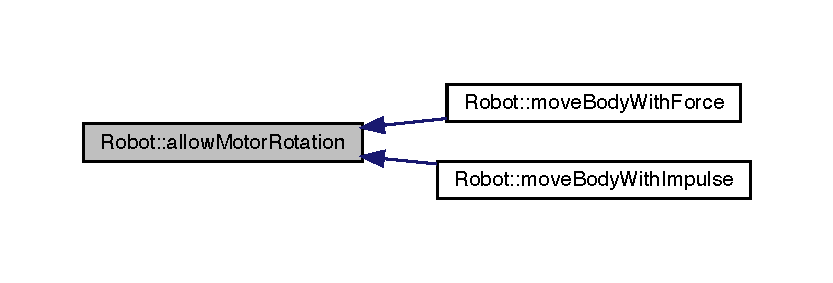
\includegraphics[width=350pt]{class_robot_afd7710fdb80993a6b6cc1aa9b88ed06a_icgraph}
\end{center}
\end{figure}
\mbox{\Hypertarget{class_robot_af11fa20795b6b4d07811f3d3089beb48}\label{class_robot_af11fa20795b6b4d07811f3d3089beb48}} 
\index{Robot@{Robot}!block\+Motor\+Rotation@{block\+Motor\+Rotation}}
\index{block\+Motor\+Rotation@{block\+Motor\+Rotation}!Robot@{Robot}}
\subsubsection{\texorpdfstring{block\+Motor\+Rotation()}{blockMotorRotation()}}
{\footnotesize\ttfamily void Robot\+::block\+Motor\+Rotation (\begin{DoxyParamCaption}\item[{\mbox{\hyperlink{_robot_8h_afc015eff6557e84151d2e53b94375445}{side}}}]{s }\end{DoxyParamCaption})}

block\+Motor\+Rotation keep the motor enable but set an infinitesimal rotation limit and the speed to 0 in order to block totally the rotation 
\begin{DoxyParams}{Parameters}
{\em s} & is the motor side can take L\+E\+FT or R\+I\+G\+HT value \\
\hline
\end{DoxyParams}
\mbox{\Hypertarget{class_robot_a27c9de7d6dcb6ca98fcbe3aa7c55bf9a}\label{class_robot_a27c9de7d6dcb6ca98fcbe3aa7c55bf9a}} 
\index{Robot@{Robot}!check\+Gripp@{check\+Gripp}}
\index{check\+Gripp@{check\+Gripp}!Robot@{Robot}}
\subsubsection{\texorpdfstring{check\+Gripp()}{checkGripp()}}
{\footnotesize\ttfamily bool Robot\+::check\+Gripp (\begin{DoxyParamCaption}\item[{\mbox{\hyperlink{_robot_8h_afc015eff6557e84151d2e53b94375445}{side}}}]{s }\end{DoxyParamCaption})}

Check if the robot is currently grabbing something (gripper on) 
\begin{DoxyParams}{Parameters}
{\em side} & of the gripper can be either L\+E\+FT or R\+I\+G\+HT \\
\hline
\end{DoxyParams}
\begin{DoxyReturn}{Returns}
true if the gripper on the side is active 
\end{DoxyReturn}
\mbox{\Hypertarget{class_robot_a7be383b14986610db597c2b26c475cbe}\label{class_robot_a7be383b14986610db597c2b26c475cbe}} 
\index{Robot@{Robot}!create\+Body@{create\+Body}}
\index{create\+Body@{create\+Body}!Robot@{Robot}}
\subsubsection{\texorpdfstring{create\+Body()}{createBody()}}
{\footnotesize\ttfamily void Robot\+::create\+Body (\begin{DoxyParamCaption}\item[{b2\+World $\ast$}]{world,  }\item[{\mbox{\hyperlink{structconfig_1_1s_robot}{config\+::s\+Robot}}}]{m\+\_\+robot\+Parameters,  }\item[{double}]{posX,  }\item[{double}]{posY,  }\item[{double}]{angle = {\ttfamily 0} }\end{DoxyParamCaption})}

Create the box2D body of the robot and attach it to the world 
\begin{DoxyParams}{Parameters}
{\em world} & box2D world defined in the main program \\
\hline
{\em robot\+Parameters} & structure containing the robot parameters\+: only the body length and speed have to be defined \\
\hline
{\em posX,posY} & \+: initial position of the robot in this world in meters \\
\hline
{\em angle} & \+: initial angle of the robot in this world in rad \\
\hline
\end{DoxyParams}
\mbox{\Hypertarget{class_robot_a3014b34d9b3da6e4a33933c937e578aa}\label{class_robot_a3014b34d9b3da6e4a33933c937e578aa}} 
\index{Robot@{Robot}!destroy\+Body@{destroy\+Body}}
\index{destroy\+Body@{destroy\+Body}!Robot@{Robot}}
\subsubsection{\texorpdfstring{destroy\+Body()}{destroyBody()}}
{\footnotesize\ttfamily void Robot\+::destroy\+Body (\begin{DoxyParamCaption}{ }\end{DoxyParamCaption})}

Destroy the Box2D bodies composing the robot. \mbox{\Hypertarget{class_robot_aae700fce06eb367ff9282492cc17ccc7}\label{class_robot_aae700fce06eb367ff9282492cc17ccc7}} 
\index{Robot@{Robot}!draw\+Body@{draw\+Body}}
\index{draw\+Body@{draw\+Body}!Robot@{Robot}}
\subsubsection{\texorpdfstring{draw\+Body()}{drawBody()}}
{\footnotesize\ttfamily void Robot\+::draw\+Body (\begin{DoxyParamCaption}\item[{sf\+::\+Render\+Window \&}]{window,  }\item[{double}]{m\+\_\+to\+\_\+pix }\end{DoxyParamCaption})}

Use S\+F\+ML to to draw the body of the robot on the window 
\begin{DoxyParams}{Parameters}
{\em window} & active S\+F\+ML window \\
\hline
{\em m\+\_\+to\+\_\+pix} & is the conversion factor used to transform the meters to pixels \\
\hline
\end{DoxyParams}
\mbox{\Hypertarget{class_robot_a99e6a9dacaae1c43f249a01485352dcf}\label{class_robot_a99e6a9dacaae1c43f249a01485352dcf}} 
\index{Robot@{Robot}!draw\+Grip\+Joint@{draw\+Grip\+Joint}}
\index{draw\+Grip\+Joint@{draw\+Grip\+Joint}!Robot@{Robot}}
\subsubsection{\texorpdfstring{draw\+Grip\+Joint()}{drawGripJoint()}}
{\footnotesize\ttfamily void Robot\+::draw\+Grip\+Joint (\begin{DoxyParamCaption}\item[{sf\+::\+Render\+Window \&}]{window,  }\item[{double}]{m\+\_\+to\+\_\+px }\end{DoxyParamCaption})}

Use S\+F\+ML to to draw the robot\textquotesingle{}s grippers on the window 
\begin{DoxyParams}{Parameters}
{\em window} & active S\+F\+ML window \\
\hline
{\em m\+\_\+to\+\_\+pix} & is the conversion factor used to transform the meters to pixels \\
\hline
\end{DoxyParams}
\mbox{\Hypertarget{class_robot_a94bec26489e5354d1b9106bbd0e59f00}\label{class_robot_a94bec26489e5354d1b9106bbd0e59f00}} 
\index{Robot@{Robot}!draw\+Joint@{draw\+Joint}}
\index{draw\+Joint@{draw\+Joint}!Robot@{Robot}}
\subsubsection{\texorpdfstring{draw\+Joint()}{drawJoint()}}
{\footnotesize\ttfamily void Robot\+::draw\+Joint (\begin{DoxyParamCaption}\item[{sf\+::\+Render\+Window \&}]{window,  }\item[{double}]{m\+\_\+to\+\_\+px }\end{DoxyParamCaption})}

Use S\+F\+ML to to draw all the joints of the robot on the window 
\begin{DoxyParams}{Parameters}
{\em window} & active S\+F\+ML window \\
\hline
{\em m\+\_\+to\+\_\+pix} & is the conversion factor used to transform the meters to pixels \\
\hline
\end{DoxyParams}
\mbox{\Hypertarget{class_robot_a41a470133819059706aab8a8d546f6bc}\label{class_robot_a41a470133819059706aab8a8d546f6bc}} 
\index{Robot@{Robot}!get\+Angle@{get\+Angle}}
\index{get\+Angle@{get\+Angle}!Robot@{Robot}}
\subsubsection{\texorpdfstring{get\+Angle()}{getAngle()}}
{\footnotesize\ttfamily double Robot\+::get\+Angle (\begin{DoxyParamCaption}{ }\end{DoxyParamCaption})}

Get the robot angle (angle of the robot body) in rad respectively to the original angle. This angle might require to be processed to be comprised between 0 and 2\+Pi \begin{DoxyReturn}{Returns}
the angle of the robot (rad) 
\end{DoxyReturn}
Here is the caller graph for this function\+:\nopagebreak
\begin{figure}[H]
\begin{center}
\leavevmode
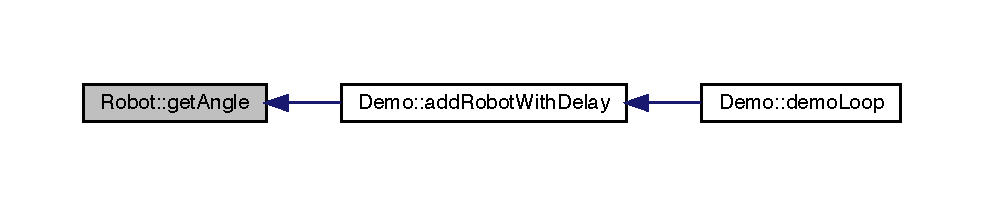
\includegraphics[width=350pt]{class_robot_a41a470133819059706aab8a8d546f6bc_icgraph}
\end{center}
\end{figure}
\mbox{\Hypertarget{class_robot_a0ccd9dbef98a3d5bf6b29d8cd781bd25}\label{class_robot_a0ccd9dbef98a3d5bf6b29d8cd781bd25}} 
\index{Robot@{Robot}!get\+Body@{get\+Body}}
\index{get\+Body@{get\+Body}!Robot@{Robot}}
\subsubsection{\texorpdfstring{get\+Body()}{getBody()}}
{\footnotesize\ttfamily b2\+Body $\ast$ Robot\+::get\+Body (\begin{DoxyParamCaption}{ }\end{DoxyParamCaption})}

Get the Box2D body part representing the attach between the robot\textquotesingle{}s wheels \begin{DoxyReturn}{Returns}
a pointer on the body of the attach between the two wheels 
\end{DoxyReturn}
Here is the caller graph for this function\+:\nopagebreak
\begin{figure}[H]
\begin{center}
\leavevmode
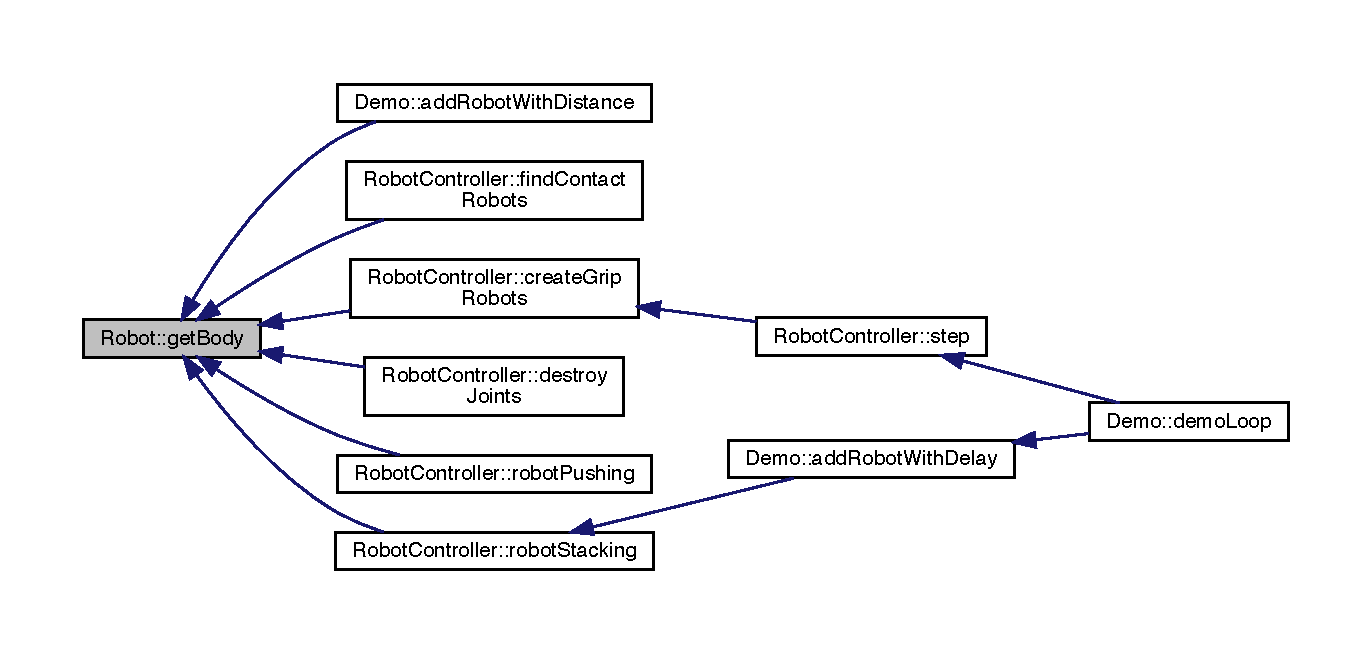
\includegraphics[width=350pt]{class_robot_a0ccd9dbef98a3d5bf6b29d8cd781bd25_icgraph}
\end{center}
\end{figure}
\mbox{\Hypertarget{class_robot_af0254cdb4fd2d60279f7b6b12a12bc4e}\label{class_robot_af0254cdb4fd2d60279f7b6b12a12bc4e}} 
\index{Robot@{Robot}!get\+Body\+Length@{get\+Body\+Length}}
\index{get\+Body\+Length@{get\+Body\+Length}!Robot@{Robot}}
\subsubsection{\texorpdfstring{get\+Body\+Length()}{getBodyLength()}}
{\footnotesize\ttfamily double Robot\+::get\+Body\+Length (\begin{DoxyParamCaption}{ }\end{DoxyParamCaption})}

\begin{DoxyReturn}{Returns}
the body length of the robot in meter (and not pixels) 
\end{DoxyReturn}
\mbox{\Hypertarget{class_robot_ad9b03690ffb189f0990dacb813b2b72c}\label{class_robot_ad9b03690ffb189f0990dacb813b2b72c}} 
\index{Robot@{Robot}!get\+Delay@{get\+Delay}}
\index{get\+Delay@{get\+Delay}!Robot@{Robot}}
\subsubsection{\texorpdfstring{get\+Delay()}{getDelay()}}
{\footnotesize\ttfamily int Robot\+::get\+Delay (\begin{DoxyParamCaption}{ }\end{DoxyParamCaption})}

Get the current robot\textquotesingle{}s delay as a number of iteration left for the robot before being able to be ready. \begin{DoxyReturn}{Returns}
the current robot\textquotesingle{}s delay before being ready 
\end{DoxyReturn}
Here is the caller graph for this function\+:\nopagebreak
\begin{figure}[H]
\begin{center}
\leavevmode
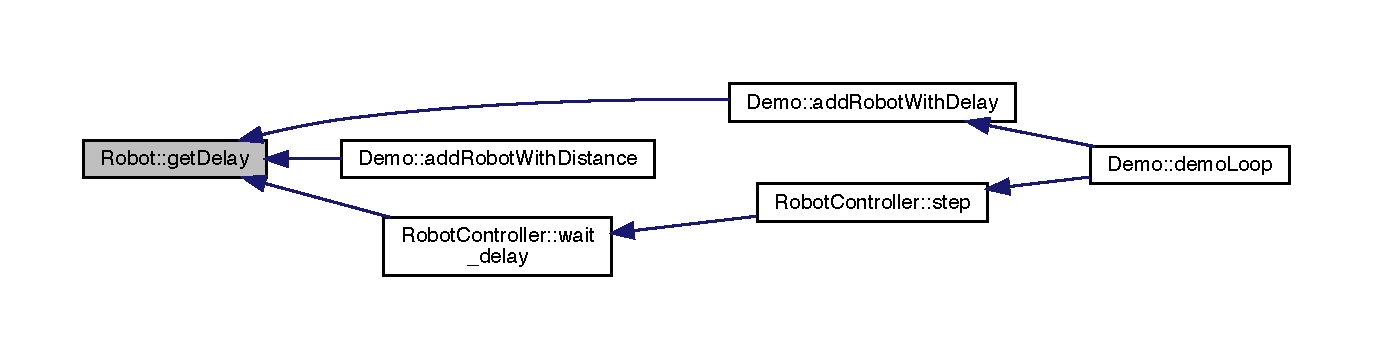
\includegraphics[width=350pt]{class_robot_ad9b03690ffb189f0990dacb813b2b72c_icgraph}
\end{center}
\end{figure}
\mbox{\Hypertarget{class_robot_a8d1d94c9cab78a96851785b1679cd457}\label{class_robot_a8d1d94c9cab78a96851785b1679cd457}} 
\index{Robot@{Robot}!get\+Id@{get\+Id}}
\index{get\+Id@{get\+Id}!Robot@{Robot}}
\subsubsection{\texorpdfstring{get\+Id()}{getId()}}
{\footnotesize\ttfamily int Robot\+::get\+Id (\begin{DoxyParamCaption}{ }\end{DoxyParamCaption})}

\begin{DoxyReturn}{Returns}
the value of the robot unique id stored in m\+\_\+id 
\end{DoxyReturn}
Here is the caller graph for this function\+:\nopagebreak
\begin{figure}[H]
\begin{center}
\leavevmode
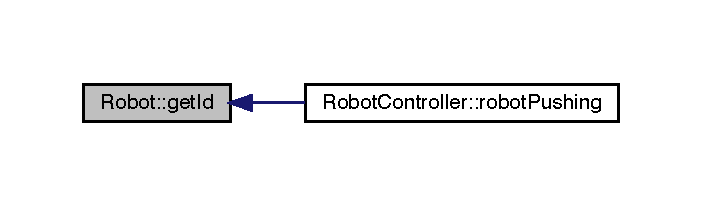
\includegraphics[width=337pt]{class_robot_a8d1d94c9cab78a96851785b1679cd457_icgraph}
\end{center}
\end{figure}
\mbox{\Hypertarget{class_robot_a536c96ba5f6c7d8f04d86a50b1adcd72}\label{class_robot_a536c96ba5f6c7d8f04d86a50b1adcd72}} 
\index{Robot@{Robot}!get\+Joint\+Def@{get\+Joint\+Def}}
\index{get\+Joint\+Def@{get\+Joint\+Def}!Robot@{Robot}}
\subsubsection{\texorpdfstring{get\+Joint\+Def()}{getJointDef()}}
{\footnotesize\ttfamily b2\+Prismatic\+Joint\+Def Robot\+::get\+Joint\+Def (\begin{DoxyParamCaption}\item[{\mbox{\hyperlink{_robot_8h_afc015eff6557e84151d2e53b94375445}{side}}}]{s }\end{DoxyParamCaption})}

get the box2D definition of the prismatic joint used to create the gripper, this definition can then be used to create the actual grip joint 
\begin{DoxyParams}{Parameters}
{\em s} & is the side of the robot (relative to the robot referential), can be either L\+E\+FT or R\+I\+G\+HT \\
\hline
\end{DoxyParams}
Here is the caller graph for this function\+:\nopagebreak
\begin{figure}[H]
\begin{center}
\leavevmode
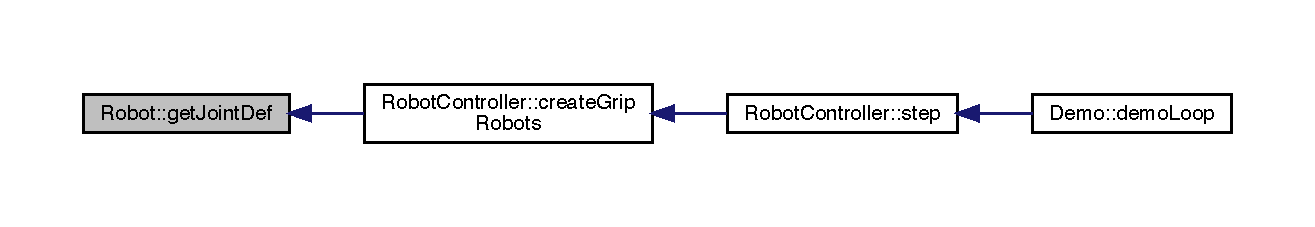
\includegraphics[width=350pt]{class_robot_a536c96ba5f6c7d8f04d86a50b1adcd72_icgraph}
\end{center}
\end{figure}
\mbox{\Hypertarget{class_robot_aafe55f24c0b2ba70dc915362abd46485}\label{class_robot_aafe55f24c0b2ba70dc915362abd46485}} 
\index{Robot@{Robot}!get\+Motor@{get\+Motor}}
\index{get\+Motor@{get\+Motor}!Robot@{Robot}}
\subsubsection{\texorpdfstring{get\+Motor()}{getMotor()}}
{\footnotesize\ttfamily b2\+Revolute\+Joint $\ast$ Robot\+::get\+Motor (\begin{DoxyParamCaption}\item[{\mbox{\hyperlink{_robot_8h_afc015eff6557e84151d2e53b94375445}{side}}}]{s }\end{DoxyParamCaption})}

Get a pointer on the Box2D joint between a foot and the robot body that act as the motor. 
\begin{DoxyParams}{Parameters}
{\em s} & side of the robot \\
\hline
\end{DoxyParams}
\begin{DoxyReturn}{Returns}
a pointer on the Box2D joint that act as the motor of the given side s 
\end{DoxyReturn}
\mbox{\Hypertarget{class_robot_af8bdea28202e00ebf48187b8943b245c}\label{class_robot_af8bdea28202e00ebf48187b8943b245c}} 
\index{Robot@{Robot}!get\+Position@{get\+Position}}
\index{get\+Position@{get\+Position}!Robot@{Robot}}
\subsubsection{\texorpdfstring{get\+Position()}{getPosition()}}
{\footnotesize\ttfamily b2\+Vec2 Robot\+::get\+Position (\begin{DoxyParamCaption}{ }\end{DoxyParamCaption})}

Get the robot center position (located at the center of the robot body) in m respectively to the origin of the Box2D world (top left corner) \begin{DoxyReturn}{Returns}
a b2\+Vec2 vector with the x and y coordinates of the robot position (m) 
\end{DoxyReturn}
Here is the caller graph for this function\+:\nopagebreak
\begin{figure}[H]
\begin{center}
\leavevmode
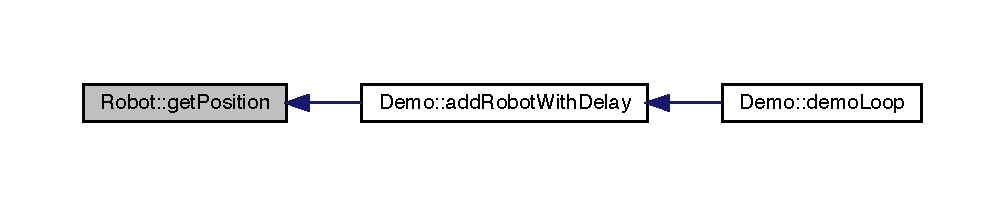
\includegraphics[width=350pt]{class_robot_af8bdea28202e00ebf48187b8943b245c_icgraph}
\end{center}
\end{figure}
\mbox{\Hypertarget{class_robot_a65b9be1d9d45b004a6ea500dd5f85246}\label{class_robot_a65b9be1d9d45b004a6ea500dd5f85246}} 
\index{Robot@{Robot}!get\+State@{get\+State}}
\index{get\+State@{get\+State}!Robot@{Robot}}
\subsubsection{\texorpdfstring{get\+State()}{getState()}}
{\footnotesize\ttfamily \mbox{\hyperlink{_robot_8h_a74a75e4700f1f71bb89d80765319e57b}{e\+\_\+state}} Robot\+::get\+State (\begin{DoxyParamCaption}{ }\end{DoxyParamCaption})}

Access the current robot state \begin{DoxyReturn}{Returns}
the e\+\_\+state value defining the robot state, can take two values W\+A\+LK or B\+R\+I\+D\+GE 
\end{DoxyReturn}
Here is the caller graph for this function\+:\nopagebreak
\begin{figure}[H]
\begin{center}
\leavevmode
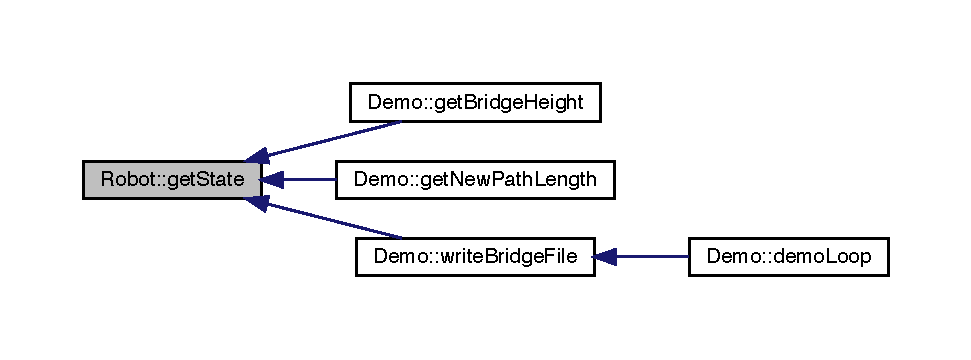
\includegraphics[width=350pt]{class_robot_a65b9be1d9d45b004a6ea500dd5f85246_icgraph}
\end{center}
\end{figure}
\mbox{\Hypertarget{class_robot_a7c5ede93bcb2007be1f2bd6b2137f271}\label{class_robot_a7c5ede93bcb2007be1f2bd6b2137f271}} 
\index{Robot@{Robot}!get\+Wheel@{get\+Wheel}}
\index{get\+Wheel@{get\+Wheel}!Robot@{Robot}}
\subsubsection{\texorpdfstring{get\+Wheel()}{getWheel()}}
{\footnotesize\ttfamily b2\+Body $\ast$ Robot\+::get\+Wheel (\begin{DoxyParamCaption}\item[{\mbox{\hyperlink{_robot_8h_afc015eff6557e84151d2e53b94375445}{side}}}]{s }\end{DoxyParamCaption})}

Get the Box2D body part representing one of the two wheels of the robot 
\begin{DoxyParams}{Parameters}
{\em s} & is the side of the robot (relative to the robot referential), can be either L\+E\+FT or R\+I\+G\+HT that define which wheel will be returned \\
\hline
\end{DoxyParams}
\begin{DoxyReturn}{Returns}
a pointer on the box2D wheel on the s side 
\end{DoxyReturn}
Here is the caller graph for this function\+:\nopagebreak
\begin{figure}[H]
\begin{center}
\leavevmode
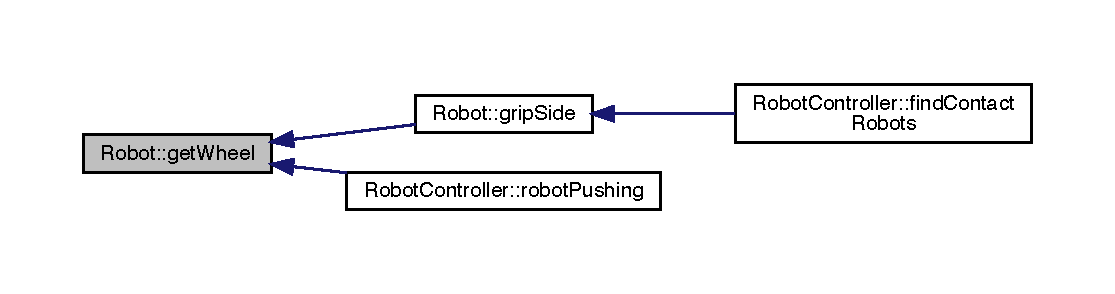
\includegraphics[width=350pt]{class_robot_a7c5ede93bcb2007be1f2bd6b2137f271_icgraph}
\end{center}
\end{figure}
\mbox{\Hypertarget{class_robot_acf8f6c6260669a8568aa0d65404e3533}\label{class_robot_acf8f6c6260669a8568aa0d65404e3533}} 
\index{Robot@{Robot}!grip@{grip}}
\index{grip@{grip}!Robot@{Robot}}
\subsubsection{\texorpdfstring{grip()}{grip()}}
{\footnotesize\ttfamily void Robot\+::grip (\begin{DoxyParamCaption}\item[{b2\+Contact $\ast$}]{contact,  }\item[{b2\+Body $\ast$}]{other\+Body,  }\item[{double}]{m\+\_\+to\+\_\+px }\end{DoxyParamCaption})}

Create the grip joint definition as a Box2D prismatic joint definition object. grip\+Ground\+From\+Pos is used when one needs to create a static robot\+: It directly create the joint object without the intermediate definition. 
\begin{DoxyParams}{Parameters}
{\em contact} & box2D contact object usually obtained via the contact listener \\
\hline
{\em other\+Body} & box2D body in contact with the robot \\
\hline
{\em m\+\_\+to\+\_\+px} & scale conversion between box2d and sfml coordinates, used to draw the contact point\\
\hline
\end{DoxyParams}
update m\+\_\+left\+Grip\+Joint\+Def and m\+\_\+right\+Grip\+Joint\+Def depending on the contact side \mbox{\Hypertarget{class_robot_abf3907d53fca6572e6984b22515c69a7}\label{class_robot_abf3907d53fca6572e6984b22515c69a7}} 
\index{Robot@{Robot}!grip\+Ground\+From\+Pos@{grip\+Ground\+From\+Pos}}
\index{grip\+Ground\+From\+Pos@{grip\+Ground\+From\+Pos}!Robot@{Robot}}
\subsubsection{\texorpdfstring{grip\+Ground\+From\+Pos()}{gripGroundFromPos()}}
{\footnotesize\ttfamily void Robot\+::grip\+Ground\+From\+Pos (\begin{DoxyParamCaption}{ }\end{DoxyParamCaption})}

Create the grip joint definition as a Box2D prismatic joint definition object. grip\+Ground\+From\+Pos is used when one needs to create a static robot\+: It directly create the joint object without the intermediate definition. 
\begin{DoxyParams}{Parameters}
{\em contact} & box2D contact object usually obtained via the contact listener \\
\hline
{\em other\+Body} & box2D body in contact with the robot \\
\hline
{\em m\+\_\+to\+\_\+px} & scale conversion between box2d and sfml coordinates, used to draw the contact point\\
\hline
\end{DoxyParams}
update m\+\_\+left\+Grip\+Joint\+Def and m\+\_\+right\+Grip\+Joint\+Def depending on the contact side \mbox{\Hypertarget{class_robot_aed1ba5683c53ac2b7e4a6c3fc7bcadba}\label{class_robot_aed1ba5683c53ac2b7e4a6c3fc7bcadba}} 
\index{Robot@{Robot}!grip\+Side@{grip\+Side}}
\index{grip\+Side@{grip\+Side}!Robot@{Robot}}
\subsubsection{\texorpdfstring{grip\+Side()}{gripSide()}}
{\footnotesize\ttfamily bool Robot\+::grip\+Side (\begin{DoxyParamCaption}\item[{b2\+Contact $\ast$}]{contact,  }\item[{b2\+Body $\ast$}]{other\+Body,  }\item[{double}]{m\+\_\+to\+\_\+px }\end{DoxyParamCaption})}

Create the grip joint definition as a Box2D prismatic joint definition object. grip\+Ground\+From\+Pos is used when one needs to create a static robot\+: It directly create the joint object without the intermediate definition. 
\begin{DoxyParams}{Parameters}
{\em contact} & box2D contact object usually obtained via the contact listener \\
\hline
{\em other\+Body} & box2D body in contact with the robot \\
\hline
{\em m\+\_\+to\+\_\+px} & scale conversion between box2d and sfml coordinates, used to draw the contact point\\
\hline
\end{DoxyParams}
update m\+\_\+left\+Grip\+Joint\+Def and m\+\_\+right\+Grip\+Joint\+Def depending on the contact side Here is the call graph for this function\+:\nopagebreak
\begin{figure}[H]
\begin{center}
\leavevmode
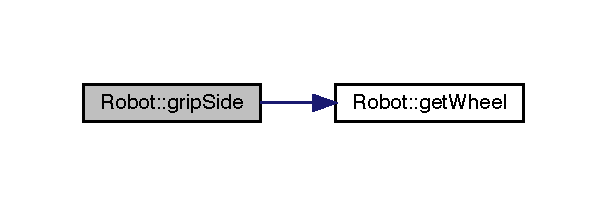
\includegraphics[width=291pt]{class_robot_aed1ba5683c53ac2b7e4a6c3fc7bcadba_cgraph}
\end{center}
\end{figure}
Here is the caller graph for this function\+:\nopagebreak
\begin{figure}[H]
\begin{center}
\leavevmode
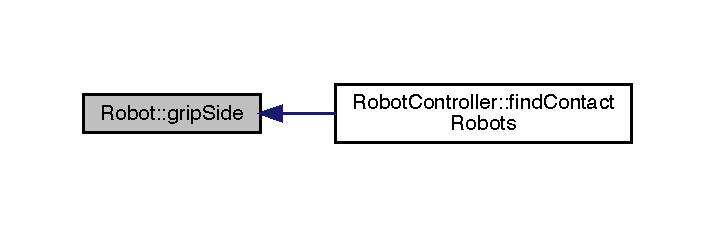
\includegraphics[width=343pt]{class_robot_aed1ba5683c53ac2b7e4a6c3fc7bcadba_icgraph}
\end{center}
\end{figure}
\mbox{\Hypertarget{class_robot_af5b6b2dc9efa49654cf80abe298cc6f9}\label{class_robot_af5b6b2dc9efa49654cf80abe298cc6f9}} 
\index{Robot@{Robot}!increment\+Nb\+Joint@{increment\+Nb\+Joint}}
\index{increment\+Nb\+Joint@{increment\+Nb\+Joint}!Robot@{Robot}}
\subsubsection{\texorpdfstring{increment\+Nb\+Joint()}{incrementNbJoint()}}
{\footnotesize\ttfamily void Robot\+::increment\+Nb\+Joint (\begin{DoxyParamCaption}\item[{\mbox{\hyperlink{_robot_8h_afc015eff6557e84151d2e53b94375445}{side}}}]{s }\end{DoxyParamCaption})}

Methods to increment the number of grip joints of the robot of a given side, this number should not exceed 1 
\begin{DoxyParams}{Parameters}
{\em s} & is the side of the robot\+: can be either L\+E\+FT or R\+I\+G\+HT \\
\hline
\end{DoxyParams}
Here is the caller graph for this function\+:\nopagebreak
\begin{figure}[H]
\begin{center}
\leavevmode
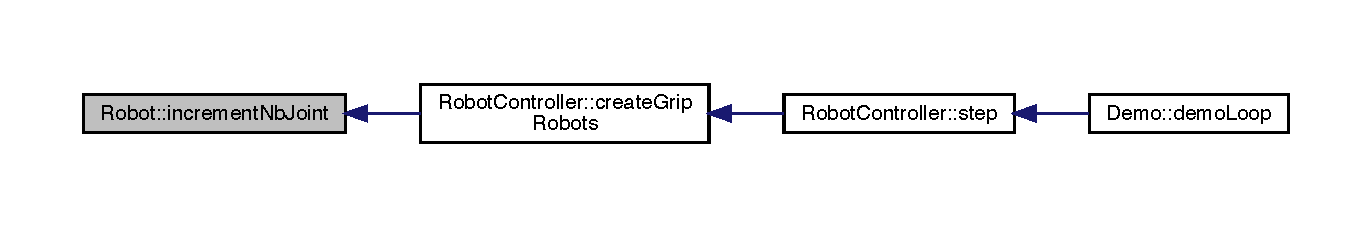
\includegraphics[width=350pt]{class_robot_af5b6b2dc9efa49654cf80abe298cc6f9_icgraph}
\end{center}
\end{figure}
\mbox{\Hypertarget{class_robot_add038ac4b424821791781171a9a45de4}\label{class_robot_add038ac4b424821791781171a9a45de4}} 
\index{Robot@{Robot}!is\+Contact@{is\+Contact}}
\index{is\+Contact@{is\+Contact}!Robot@{Robot}}
\subsubsection{\texorpdfstring{is\+Contact()}{isContact()}}
{\footnotesize\ttfamily bool Robot\+::is\+Contact (\begin{DoxyParamCaption}{ }\end{DoxyParamCaption})}

\begin{DoxyReturn}{Returns}
true if the robot has just initiated a contact and didn\textquotesingle{}t create a joint yet. 
\end{DoxyReturn}
Here is the caller graph for this function\+:\nopagebreak
\begin{figure}[H]
\begin{center}
\leavevmode
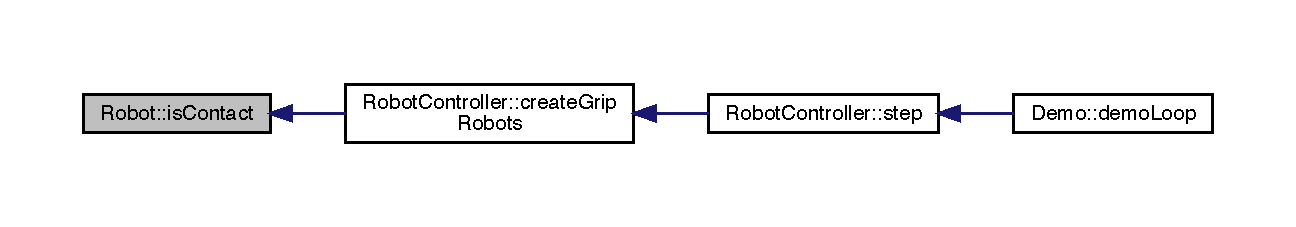
\includegraphics[width=350pt]{class_robot_add038ac4b424821791781171a9a45de4_icgraph}
\end{center}
\end{figure}
\mbox{\Hypertarget{class_robot_a156c0ecf0bed5e117335d4c1c12d2d06}\label{class_robot_a156c0ecf0bed5e117335d4c1c12d2d06}} 
\index{Robot@{Robot}!is\+Grabbed@{is\+Grabbed}}
\index{is\+Grabbed@{is\+Grabbed}!Robot@{Robot}}
\subsubsection{\texorpdfstring{is\+Grabbed()}{isGrabbed()}}
{\footnotesize\ttfamily bool Robot\+::is\+Grabbed (\begin{DoxyParamCaption}{ }\end{DoxyParamCaption})}

Check if the robot is currently grabbed by another robot \begin{DoxyReturn}{Returns}
true if it is 
\end{DoxyReturn}
Here is the caller graph for this function\+:\nopagebreak
\begin{figure}[H]
\begin{center}
\leavevmode
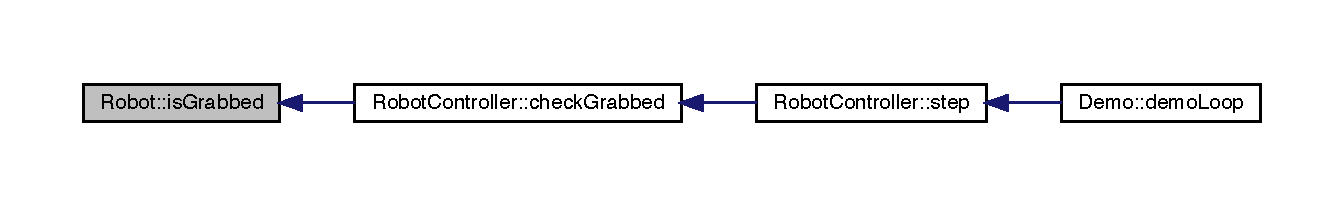
\includegraphics[width=350pt]{class_robot_a156c0ecf0bed5e117335d4c1c12d2d06_icgraph}
\end{center}
\end{figure}
\mbox{\Hypertarget{class_robot_a885b7c6b9da718dfe4eb53802adfce92}\label{class_robot_a885b7c6b9da718dfe4eb53802adfce92}} 
\index{Robot@{Robot}!is\+Moving@{is\+Moving}}
\index{is\+Moving@{is\+Moving}!Robot@{Robot}}
\subsubsection{\texorpdfstring{is\+Moving()}{isMoving()}}
{\footnotesize\ttfamily bool Robot\+::is\+Moving (\begin{DoxyParamCaption}{ }\end{DoxyParamCaption})}

\begin{DoxyReturn}{Returns}
true if the robot is moving, false otherwise 
\end{DoxyReturn}
Here is the caller graph for this function\+:\nopagebreak
\begin{figure}[H]
\begin{center}
\leavevmode
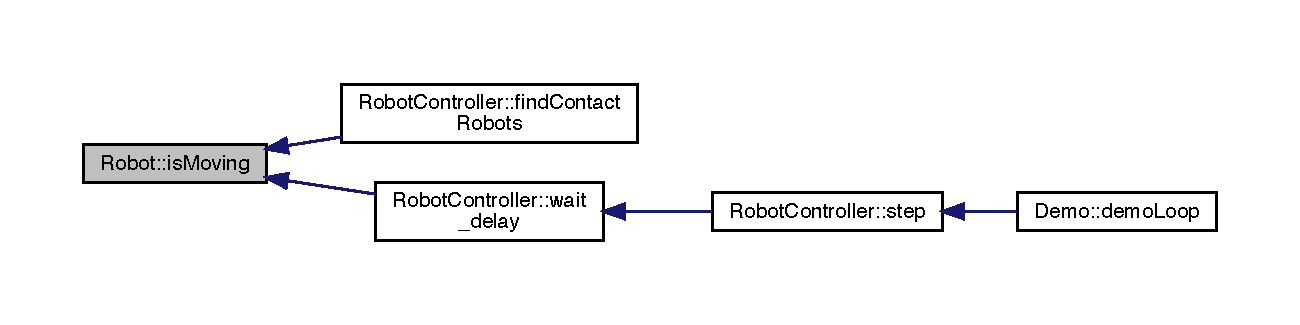
\includegraphics[width=350pt]{class_robot_a885b7c6b9da718dfe4eb53802adfce92_icgraph}
\end{center}
\end{figure}
\mbox{\Hypertarget{class_robot_a521b65cb8bc45f7eae7bdaae0cd0f847}\label{class_robot_a521b65cb8bc45f7eae7bdaae0cd0f847}} 
\index{Robot@{Robot}!is\+Ready@{is\+Ready}}
\index{is\+Ready@{is\+Ready}!Robot@{Robot}}
\subsubsection{\texorpdfstring{is\+Ready()}{isReady()}}
{\footnotesize\ttfamily bool Robot\+::is\+Ready (\begin{DoxyParamCaption}{ }\end{DoxyParamCaption})}

\begin{DoxyReturn}{Returns}
true if the robot is ready to move, false otherwise 
\end{DoxyReturn}
\mbox{\Hypertarget{class_robot_aec072eed2d38baedbbd5132b760720d0}\label{class_robot_aec072eed2d38baedbbd5132b760720d0}} 
\index{Robot@{Robot}!limit\+Motor\+Rotation@{limit\+Motor\+Rotation}}
\index{limit\+Motor\+Rotation@{limit\+Motor\+Rotation}!Robot@{Robot}}
\subsubsection{\texorpdfstring{limit\+Motor\+Rotation()}{limitMotorRotation()}}
{\footnotesize\ttfamily void Robot\+::limit\+Motor\+Rotation (\begin{DoxyParamCaption}\item[{\mbox{\hyperlink{_robot_8h_afc015eff6557e84151d2e53b94375445}{side}}}]{s,  }\item[{double}]{limit\+\_\+angle\+\_\+rad }\end{DoxyParamCaption})}

Limit the motor rotation between +/-\/ a given limit angle around the reference angle. The reference angle is defined by the member attribute m\+\_\+reference\+Angle\+Joint 
\begin{DoxyParams}{Parameters}
{\em s} & is the motor side can take L\+E\+FT or R\+I\+G\+HT value \\
\hline
{\em limit\+\_\+angle\+\_\+rad} & is the value that define the limit angle in rad \\
\hline
\end{DoxyParams}
\mbox{\Hypertarget{class_robot_ab713edf012849220f5096ea4b2d3e110}\label{class_robot_ab713edf012849220f5096ea4b2d3e110}} 
\index{Robot@{Robot}!move\+Body\+With\+Force@{move\+Body\+With\+Force}}
\index{move\+Body\+With\+Force@{move\+Body\+With\+Force}!Robot@{Robot}}
\subsubsection{\texorpdfstring{move\+Body\+With\+Force()}{moveBodyWithForce()}}
{\footnotesize\ttfamily void Robot\+::move\+Body\+With\+Force (\begin{DoxyParamCaption}{ }\end{DoxyParamCaption})}

Second of the three different methods to move the robot body in the clockwise direction, The parameters might need to be adapted to fit the simulation parameters (object size, scale, weight...) The speed is applied via the m\+\_\+angular\+Speed class member (except for the force The impulse method uses a proportional action to reach the angular target speed Here is the call graph for this function\+:\nopagebreak
\begin{figure}[H]
\begin{center}
\leavevmode
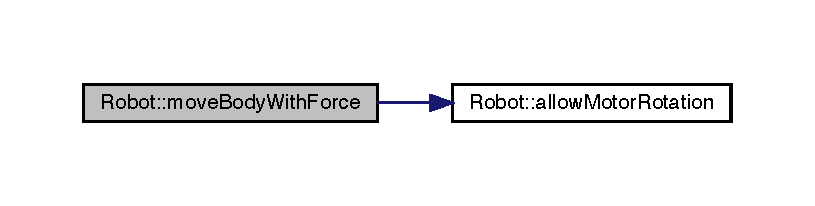
\includegraphics[width=350pt]{class_robot_ab713edf012849220f5096ea4b2d3e110_cgraph}
\end{center}
\end{figure}
\mbox{\Hypertarget{class_robot_a2d8a6b3ef3bd324ac69119f80dc9f305}\label{class_robot_a2d8a6b3ef3bd324ac69119f80dc9f305}} 
\index{Robot@{Robot}!move\+Body\+With\+Impulse@{move\+Body\+With\+Impulse}}
\index{move\+Body\+With\+Impulse@{move\+Body\+With\+Impulse}!Robot@{Robot}}
\subsubsection{\texorpdfstring{move\+Body\+With\+Impulse()}{moveBodyWithImpulse()}}
{\footnotesize\ttfamily void Robot\+::move\+Body\+With\+Impulse (\begin{DoxyParamCaption}{ }\end{DoxyParamCaption})}

Third of the three different methods to move the robot body in the clockwise direction, The parameters might need to be adapted to fit the simulation parameters (object size, scale, weight...) The speed is applied via the m\+\_\+angular\+Speed class member (except for the force The impulse method uses a proportional action to reach the angular target speed Here is the call graph for this function\+:\nopagebreak
\begin{figure}[H]
\begin{center}
\leavevmode
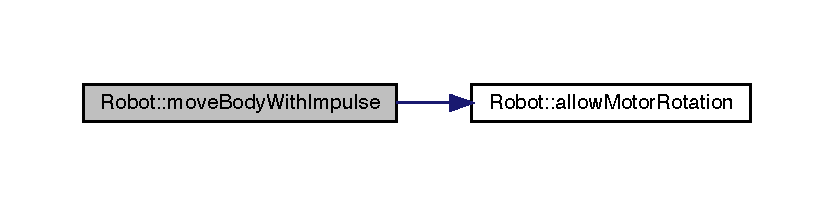
\includegraphics[width=350pt]{class_robot_a2d8a6b3ef3bd324ac69119f80dc9f305_cgraph}
\end{center}
\end{figure}
\mbox{\Hypertarget{class_robot_a55036d85a36c4e8ed3ff6f8381331c70}\label{class_robot_a55036d85a36c4e8ed3ff6f8381331c70}} 
\index{Robot@{Robot}!move\+Body\+With\+Motor@{move\+Body\+With\+Motor}}
\index{move\+Body\+With\+Motor@{move\+Body\+With\+Motor}!Robot@{Robot}}
\subsubsection{\texorpdfstring{move\+Body\+With\+Motor()}{moveBodyWithMotor()}}
{\footnotesize\ttfamily void Robot\+::move\+Body\+With\+Motor (\begin{DoxyParamCaption}{ }\end{DoxyParamCaption})}

First of the three different methods to move the robot body in the clockwise direction, This is the one used in the current implementation, the other two functions are alternative way to move the body but are currently not used The speed is applied via the m\+\_\+angular\+Speed class member (except for the force The impulse method uses a proportional action to reach the angular target speed \mbox{\Hypertarget{class_robot_ae6f0f49e30cf9c65605f6a75f390ec52}\label{class_robot_ae6f0f49e30cf9c65605f6a75f390ec52}} 
\index{Robot@{Robot}!nb\+Joint@{nb\+Joint}}
\index{nb\+Joint@{nb\+Joint}!Robot@{Robot}}
\subsubsection{\texorpdfstring{nb\+Joint()}{nbJoint()}}
{\footnotesize\ttfamily int Robot\+::nb\+Joint (\begin{DoxyParamCaption}\item[{\mbox{\hyperlink{_robot_8h_afc015eff6557e84151d2e53b94375445}{side}}}]{s }\end{DoxyParamCaption})}

Methods to check the number of grip joints of the robot of a given side, this number should not exceed 1 
\begin{DoxyParams}{Parameters}
{\em s} & is the side of the robot\+: can be either L\+E\+FT or R\+I\+G\+HT \\
\hline
\end{DoxyParams}
Here is the caller graph for this function\+:\nopagebreak
\begin{figure}[H]
\begin{center}
\leavevmode
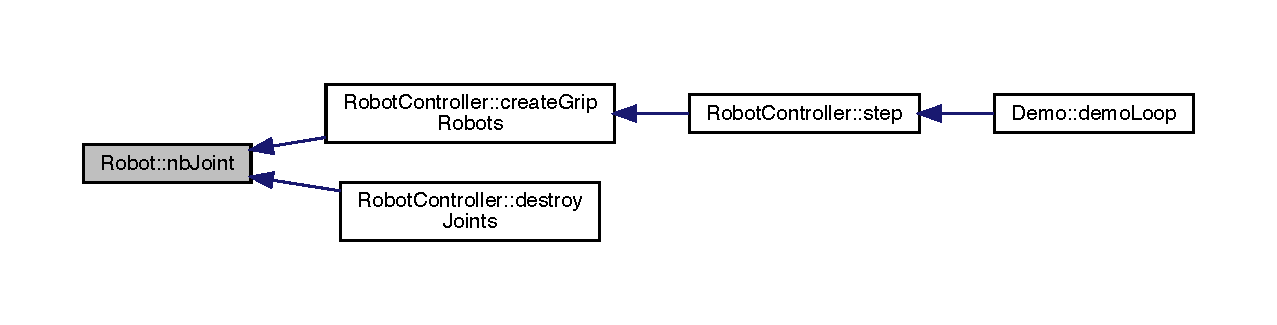
\includegraphics[width=350pt]{class_robot_ae6f0f49e30cf9c65605f6a75f390ec52_icgraph}
\end{center}
\end{figure}
\mbox{\Hypertarget{class_robot_abbba5cddb2dc90005c26b99d968f102d}\label{class_robot_abbba5cddb2dc90005c26b99d968f102d}} 
\index{Robot@{Robot}!reset\+Nb\+Joint@{reset\+Nb\+Joint}}
\index{reset\+Nb\+Joint@{reset\+Nb\+Joint}!Robot@{Robot}}
\subsubsection{\texorpdfstring{reset\+Nb\+Joint()}{resetNbJoint()}}
{\footnotesize\ttfamily void Robot\+::reset\+Nb\+Joint (\begin{DoxyParamCaption}\item[{\mbox{\hyperlink{_robot_8h_afc015eff6557e84151d2e53b94375445}{side}}}]{s }\end{DoxyParamCaption})}

Methods to reset the number of grip joints of the robot of a given side, this number should not exceed 1 
\begin{DoxyParams}{Parameters}
{\em s} & is the side of the robot\+: can be either L\+E\+FT or R\+I\+G\+HT \\
\hline
\end{DoxyParams}
Here is the caller graph for this function\+:\nopagebreak
\begin{figure}[H]
\begin{center}
\leavevmode
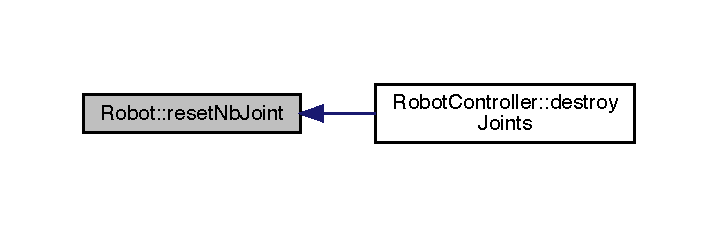
\includegraphics[width=345pt]{class_robot_abbba5cddb2dc90005c26b99d968f102d_icgraph}
\end{center}
\end{figure}
\mbox{\Hypertarget{class_robot_af0d391d121096fa6f2d214bb8910c0a1}\label{class_robot_af0d391d121096fa6f2d214bb8910c0a1}} 
\index{Robot@{Robot}!set\+Contact@{set\+Contact}}
\index{set\+Contact@{set\+Contact}!Robot@{Robot}}
\subsubsection{\texorpdfstring{set\+Contact()}{setContact()}}
{\footnotesize\ttfamily void Robot\+::set\+Contact (\begin{DoxyParamCaption}\item[{bool}]{contact }\end{DoxyParamCaption})}

Used in the contact listener to update the m\+\_\+contact flag if the robot initiate the contact

update m\+\_\+contact Here is the caller graph for this function\+:\nopagebreak
\begin{figure}[H]
\begin{center}
\leavevmode
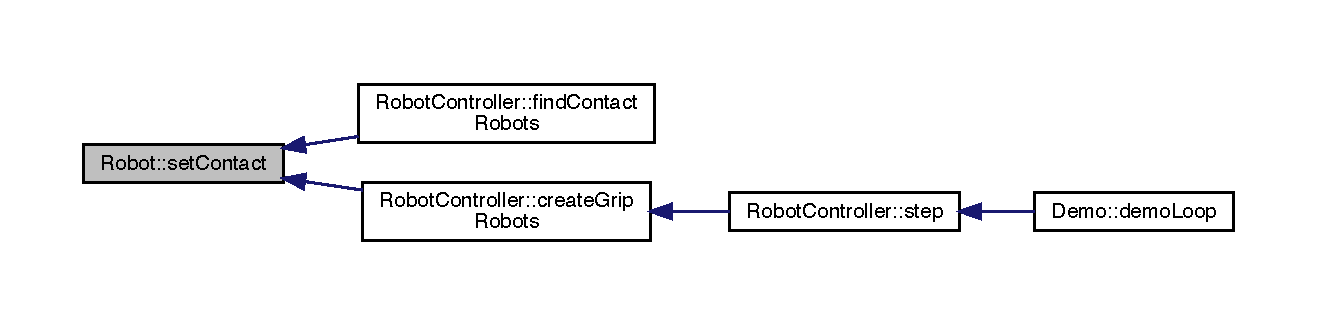
\includegraphics[width=350pt]{class_robot_af0d391d121096fa6f2d214bb8910c0a1_icgraph}
\end{center}
\end{figure}
\mbox{\Hypertarget{class_robot_a75e40c383e9191a17f25baa3aa5a35d8}\label{class_robot_a75e40c383e9191a17f25baa3aa5a35d8}} 
\index{Robot@{Robot}!set\+Delay@{set\+Delay}}
\index{set\+Delay@{set\+Delay}!Robot@{Robot}}
\subsubsection{\texorpdfstring{set\+Delay()}{setDelay()}}
{\footnotesize\ttfamily void Robot\+::set\+Delay (\begin{DoxyParamCaption}\item[{int}]{delay }\end{DoxyParamCaption})}

setter and getter of the delay m\+\_\+delay parameter 
\begin{DoxyParams}{Parameters}
{\em delay} & is the number of iteration needed to be able to turn the motors on again \\
\hline
\end{DoxyParams}
Here is the caller graph for this function\+:\nopagebreak
\begin{figure}[H]
\begin{center}
\leavevmode
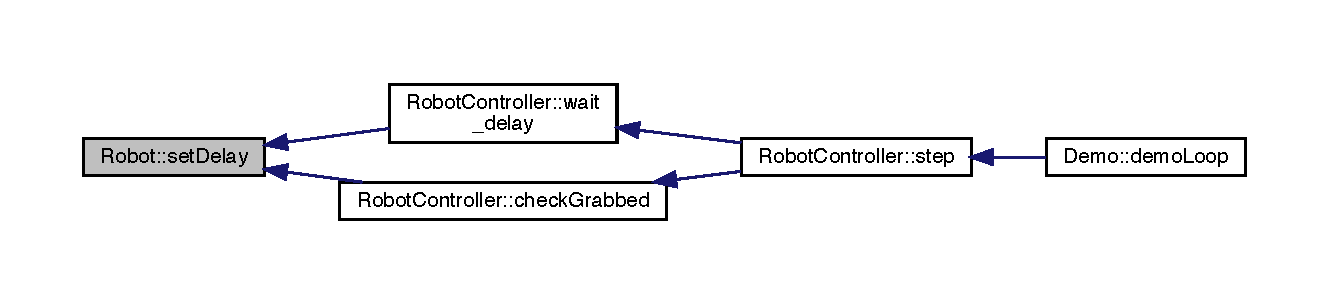
\includegraphics[width=350pt]{class_robot_a75e40c383e9191a17f25baa3aa5a35d8_icgraph}
\end{center}
\end{figure}
\mbox{\Hypertarget{class_robot_a46b12a6c9386c0067f9f35b3e60a25f7}\label{class_robot_a46b12a6c9386c0067f9f35b3e60a25f7}} 
\index{Robot@{Robot}!set\+Id@{set\+Id}}
\index{set\+Id@{set\+Id}!Robot@{Robot}}
\subsubsection{\texorpdfstring{set\+Id()}{setId()}}
{\footnotesize\ttfamily void Robot\+::set\+Id (\begin{DoxyParamCaption}\item[{int}]{id }\end{DoxyParamCaption})}

Set the unique id of the robot. Usually it corresponds to the number of robot created (as opposed to number of active robots) 
\begin{DoxyParams}{Parameters}
{\em id} & the unique id of the robot\\
\hline
\end{DoxyParams}
update m\+\_\+id \mbox{\Hypertarget{class_robot_a0a1948c69efd8bce2487afdedb6f47f1}\label{class_robot_a0a1948c69efd8bce2487afdedb6f47f1}} 
\index{Robot@{Robot}!set\+Speed@{set\+Speed}}
\index{set\+Speed@{set\+Speed}!Robot@{Robot}}
\subsubsection{\texorpdfstring{set\+Speed()}{setSpeed()}}
{\footnotesize\ttfamily void Robot\+::set\+Speed (\begin{DoxyParamCaption}\item[{double}]{speed }\end{DoxyParamCaption})}

the rotational robot speed, if the move\+Body\+With\+Motor is used, the speed is in rad/s \mbox{\Hypertarget{class_robot_aaf534f168d818112ae1f6440b329eb0a}\label{class_robot_aaf534f168d818112ae1f6440b329eb0a}} 
\index{Robot@{Robot}!set\+State@{set\+State}}
\index{set\+State@{set\+State}!Robot@{Robot}}
\subsubsection{\texorpdfstring{set\+State()}{setState()}}
{\footnotesize\ttfamily void Robot\+::set\+State (\begin{DoxyParamCaption}\item[{\mbox{\hyperlink{_robot_8h_a74a75e4700f1f71bb89d80765319e57b}{e\+\_\+state}}}]{state }\end{DoxyParamCaption})}

Set the current robot state 
\begin{DoxyParams}{Parameters}
{\em state} & is the new robot state, can take three values W\+A\+LK or B\+R\+I\+D\+GE \\
\hline
\end{DoxyParams}
Here is the caller graph for this function\+:\nopagebreak
\begin{figure}[H]
\begin{center}
\leavevmode
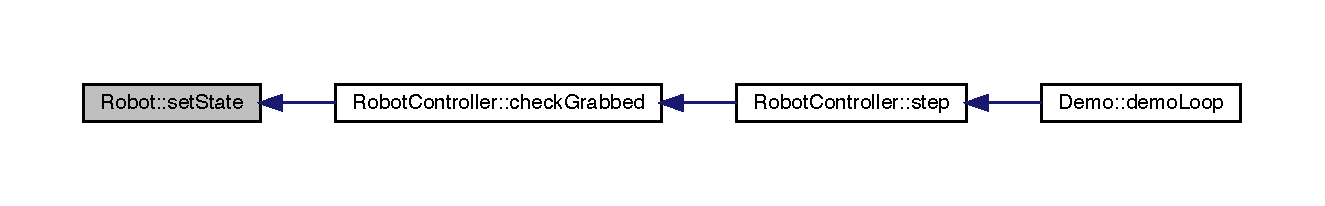
\includegraphics[width=350pt]{class_robot_aaf534f168d818112ae1f6440b329eb0a_icgraph}
\end{center}
\end{figure}
\mbox{\Hypertarget{class_robot_a4d3a07ab64d0a9289a20d40e9a9f27dc}\label{class_robot_a4d3a07ab64d0a9289a20d40e9a9f27dc}} 
\index{Robot@{Robot}!turn\+Off\+Motor@{turn\+Off\+Motor}}
\index{turn\+Off\+Motor@{turn\+Off\+Motor}!Robot@{Robot}}
\subsubsection{\texorpdfstring{turn\+Off\+Motor()}{turnOffMotor()}}
{\footnotesize\ttfamily void Robot\+::turn\+Off\+Motor (\begin{DoxyParamCaption}\item[{\mbox{\hyperlink{_robot_8h_afc015eff6557e84151d2e53b94375445}{side}}}]{s }\end{DoxyParamCaption})}

Turn off wheels\textquotesingle{} motor turn\+Off\+Motor disable the motor, it means that the rotation is freed 
\begin{DoxyParams}{Parameters}
{\em s} & is the motor side can take L\+E\+FT or R\+I\+G\+HT value \\
\hline
\end{DoxyParams}


\subsection{Member Data Documentation}
\mbox{\Hypertarget{class_robot_a35d0d222246bd7084fac5ae5cdf6d3ce}\label{class_robot_a35d0d222246bd7084fac5ae5cdf6d3ce}} 
\index{Robot@{Robot}!m\+\_\+previous\+Grip\+Joint@{m\+\_\+previous\+Grip\+Joint}}
\index{m\+\_\+previous\+Grip\+Joint@{m\+\_\+previous\+Grip\+Joint}!Robot@{Robot}}
\subsubsection{\texorpdfstring{m\+\_\+previous\+Grip\+Joint}{m\_previousGripJoint}}
{\footnotesize\ttfamily b2\+Prismatic\+Joint$\ast$ Robot\+::m\+\_\+previous\+Grip\+Joint = nullptr}

Pointers on the two possible gripping joints 

The documentation for this class was generated from the following files\+:\begin{DoxyCompactItemize}
\item 
simulation/src/\mbox{\hyperlink{_robot_8h}{Robot.\+h}}\item 
simulation/src/Robot.\+cpp\end{DoxyCompactItemize}

\hypertarget{class_robot_controller}{}\section{Robot\+Controller Class Reference}
\label{class_robot_controller}\index{Robot\+Controller@{Robot\+Controller}}
\subsection*{Public Member Functions}
\begin{DoxyCompactItemize}
\item 
\mbox{\Hypertarget{class_robot_controller_a18526d0c7d6d17c00894ef1cd8d2a974}\label{class_robot_controller_a18526d0c7d6d17c00894ef1cd8d2a974}} 
{\bfseries Robot\+Controller} (\mbox{\hyperlink{structconfig_1_1s_controller}{config\+::s\+Controller}} controller\+Param, \mbox{\hyperlink{structconfig_1_1s_robot}{config\+::s\+Robot}} robot\+Param, b2\+Body $\ast$terrain, double m\+\_\+to\+\_\+px=0)
\item 
void \mbox{\hyperlink{class_robot_controller_a1e3c66846d346e125954dd30bec8ac50}{add\+Robot}} (\mbox{\hyperlink{class_robot}{Robot}} $\ast$robot)
\item 
bool \mbox{\hyperlink{class_robot_controller_a69372797c97d6f9212dc63d2b35b4932}{check\+Grabbed}} (\mbox{\hyperlink{class_robot}{Robot}} \&robot)
\item 
\mbox{\Hypertarget{class_robot_controller_ae68c8240dde6a4f3545cfbc150bc122d}\label{class_robot_controller_ae68c8240dde6a4f3545cfbc150bc122d}} 
void {\bfseries create} (\mbox{\hyperlink{structconfig_1_1s_controller}{config\+::s\+Controller}} controller\+Param, \mbox{\hyperlink{structconfig_1_1s_robot}{config\+::s\+Robot}} robot\+Param, b2\+Body $\ast$terrain, double m\+\_\+to\+\_\+px=0)
\item 
void \mbox{\hyperlink{class_robot_controller_a6b0bdb7620acbf40f48426e30ff0b759}{create\+Grip\+Robots}} (\mbox{\hyperlink{class_robot}{Robot}} \&robot)
\item 
bool \mbox{\hyperlink{class_robot_controller_ad79af125e28750338e0da1fb35d0b72d}{create\+Robot}} (b2\+World $\ast$world, int delay, double posX, double posY, double angle=0)
\item 
void \mbox{\hyperlink{class_robot_controller_a62fac365f203e2f826efb9b7b7e56854}{destroy\+Joints}} (\mbox{\hyperlink{class_robot}{Robot}} \&robot, \mbox{\hyperlink{_robot_8h_afc015eff6557e84151d2e53b94375445}{side}} s)
\item 
void \mbox{\hyperlink{class_robot_controller_a2d4d4c93aed605c945e7a95876825bdc}{draw\+Robots}} (sf\+::\+Render\+Window \&window, double m\+\_\+to\+\_\+px)
\item 
void \mbox{\hyperlink{class_robot_controller_a11e413a1ac6466f360f46820d28b0f2e}{find\+Contact\+Robots}} (b2\+Contact $\ast$contact)
\item 
double \mbox{\hyperlink{class_robot_controller_a55f55b2b3b9013bdfc28ad11e0318ce8}{get\+Dissolution\+Time}} ()
\item 
int \mbox{\hyperlink{class_robot_controller_a45a4e25b2bb49bf2f1dc18b0f21a6f8d}{get\+Nb\+Active\+Robots}} ()
\item 
int \mbox{\hyperlink{class_robot_controller_a612d9355c9638b9f0bb24348647ada45}{get\+Nb\+Robots}} (\mbox{\hyperlink{_robot_8h_a74a75e4700f1f71bb89d80765319e57b}{e\+\_\+state}} s)
\item 
int \mbox{\hyperlink{class_robot_controller_a83a58bbd6f7fbafb3038ec0cb6271fda}{get\+Nb\+Robots\+Blocked}} ()
\item 
\mbox{\hyperlink{class_robot}{Robot}} $\ast$ \mbox{\hyperlink{class_robot_controller_ae421f813b81632c35ec3494717fd0f12}{get\+Robot}} (int pos\+\_\+id)
\item 
\mbox{\hyperlink{class_robot}{Robot}} $\ast$ \mbox{\hyperlink{class_robot_controller_aa247b8c90ab585358f07a18c891c8b31}{get\+Robot\+With\+Id}} (int id)
\item 
double \mbox{\hyperlink{class_robot_controller_acd0a73a62eca471d77a42a0c15964b8e}{get\+Stabilization\+Time}} ()
\item 
void \mbox{\hyperlink{class_robot_controller_a3191cad0cf82d3378aec0512baf2722b}{invert\+Moving\+Wheel}} (\mbox{\hyperlink{class_robot}{Robot}} \&robot)
\item 
bool \mbox{\hyperlink{class_robot_controller_a5f3c279e0082ea8dbfe03fd32d8e42b5}{is\+Bridge\+Dissolved}} ()
\item 
bool \mbox{\hyperlink{class_robot_controller_a05233232614480ea30138101f730a329}{is\+Bridge\+Stable}} ()
\item 
void \mbox{\hyperlink{class_robot_controller_a0774831ed97c92f24d082603e66950b0}{remove\+Robot}} ()
\item 
void \mbox{\hyperlink{class_robot_controller_a68972b0f0f2f033ee0d2d2c849fb38c9}{robot\+Out}} (double end\+\_\+x, int id)
\item 
bool \mbox{\hyperlink{class_robot_controller_a927abf2765cd53b39acf128f318c3fe5}{robot\+Pushing}} (\mbox{\hyperlink{class_robot}{Robot}} \&r)
\item 
bool \mbox{\hyperlink{class_robot_controller_a83d343eb8958d365624d06ac1b0b1b3d}{robot\+Stacking}} (\mbox{\hyperlink{class_robot}{Robot}} $\ast$r, float posX)
\item 
void \mbox{\hyperlink{class_robot_controller_a19191b156161bd7a3978659329ceaad2}{set\+Bridge\+Stability}} (bool stable)
\item 
void \mbox{\hyperlink{class_robot_controller_adf00a753bc750624e805f57f8998ad78}{set\+Nb\+Robots}} (int nb\+\_\+robots)
\item 
void \mbox{\hyperlink{class_robot_controller_a797837410a2802b5d7399d132924ba2c}{set\+Robot\+State}} (\mbox{\hyperlink{class_robot}{Robot}} \&robot, \mbox{\hyperlink{_robot_8h_a74a75e4700f1f71bb89d80765319e57b}{e\+\_\+state}} robot\+State)
\item 
void \mbox{\hyperlink{class_robot_controller_a76d6bb1e93bb9523850370fdf76407c4}{set\+Scale}} (double m\+\_\+to\+\_\+px)
\item 
void \mbox{\hyperlink{class_robot_controller_ab2e4091fc2e47701cc5dbd7c2d9fc649}{step}} (double end\+\_\+x)
\item 
void \mbox{\hyperlink{class_robot_controller_ae433d7a77a59e8eced35fc4885051805}{wait\+\_\+delay}} (\mbox{\hyperlink{class_robot}{Robot}} \&robot)
\end{DoxyCompactItemize}
\subsection*{Public Attributes}
\begin{DoxyCompactItemize}
\item 
bool \mbox{\hyperlink{class_robot_controller_abe09204acb8936eddcacbae0b023423a}{m\+\_\+bridge\+Entry}} = false
\end{DoxyCompactItemize}


\subsection{Member Function Documentation}
\mbox{\Hypertarget{class_robot_controller_a1e3c66846d346e125954dd30bec8ac50}\label{class_robot_controller_a1e3c66846d346e125954dd30bec8ac50}} 
\index{Robot\+Controller@{Robot\+Controller}!add\+Robot@{add\+Robot}}
\index{add\+Robot@{add\+Robot}!Robot\+Controller@{Robot\+Controller}}
\subsubsection{\texorpdfstring{add\+Robot()}{addRobot()}}
{\footnotesize\ttfamily void Robot\+Controller\+::add\+Robot (\begin{DoxyParamCaption}\item[{\mbox{\hyperlink{class_robot}{Robot}} $\ast$}]{robot }\end{DoxyParamCaption})}

Add a robot to the controller after the robot has been created. A better solution to add a robot to the simulation should be to create directly a new robot from the controller method using the create\+Robot method. 
\begin{DoxyParams}{Parameters}
{\em robot} & is a pointer on a newly created robot object. \\
\hline
\end{DoxyParams}
\mbox{\Hypertarget{class_robot_controller_a69372797c97d6f9212dc63d2b35b4932}\label{class_robot_controller_a69372797c97d6f9212dc63d2b35b4932}} 
\index{Robot\+Controller@{Robot\+Controller}!check\+Grabbed@{check\+Grabbed}}
\index{check\+Grabbed@{check\+Grabbed}!Robot\+Controller@{Robot\+Controller}}
\subsubsection{\texorpdfstring{check\+Grabbed()}{checkGrabbed()}}
{\footnotesize\ttfamily bool Robot\+Controller\+::check\+Grabbed (\begin{DoxyParamCaption}\item[{\mbox{\hyperlink{class_robot}{Robot}} \&}]{robot }\end{DoxyParamCaption})}

Check if the robot is grabbed by any other robot of the controller 
\begin{DoxyParams}{Parameters}
{\em robot} & is the robot to be tested \\
\hline
\end{DoxyParams}
\begin{DoxyReturn}{Returns}
true if the robot is grabbed, false otherwise 
\end{DoxyReturn}
Here is the call graph for this function\+:\nopagebreak
\begin{figure}[H]
\begin{center}
\leavevmode
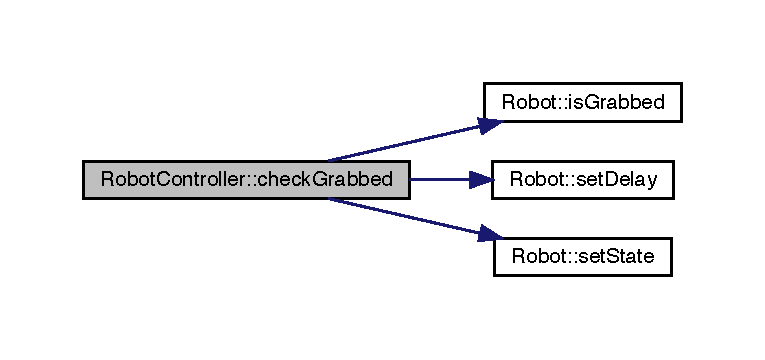
\includegraphics[width=350pt]{class_robot_controller_a69372797c97d6f9212dc63d2b35b4932_cgraph}
\end{center}
\end{figure}
Here is the caller graph for this function\+:\nopagebreak
\begin{figure}[H]
\begin{center}
\leavevmode
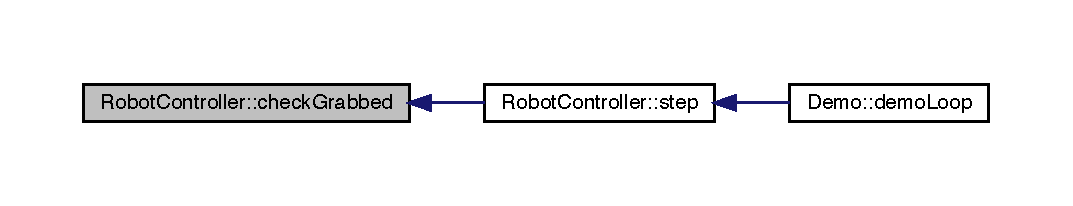
\includegraphics[width=350pt]{class_robot_controller_a69372797c97d6f9212dc63d2b35b4932_icgraph}
\end{center}
\end{figure}
\mbox{\Hypertarget{class_robot_controller_a6b0bdb7620acbf40f48426e30ff0b759}\label{class_robot_controller_a6b0bdb7620acbf40f48426e30ff0b759}} 
\index{Robot\+Controller@{Robot\+Controller}!create\+Grip\+Robots@{create\+Grip\+Robots}}
\index{create\+Grip\+Robots@{create\+Grip\+Robots}!Robot\+Controller@{Robot\+Controller}}
\subsubsection{\texorpdfstring{create\+Grip\+Robots()}{createGripRobots()}}
{\footnotesize\ttfamily void Robot\+Controller\+::create\+Grip\+Robots (\begin{DoxyParamCaption}\item[{\mbox{\hyperlink{class_robot}{Robot}} \&}]{robot }\end{DoxyParamCaption})}

Takes the robot as parameter and create a new grip in the box2D world if the robot.\+is\+Contact() is true 
\begin{DoxyParams}{Parameters}
{\em robot} & generally from the m\+\_\+robot\+Vector of the controller  \mbox{\hyperlink{class_robot_a35d0d222246bd7084fac5ae5cdf6d3ce}{Robot\+::m\+\_\+previous\+Grip\+Joint}} and Robot\+::m\+\_\+current\+Grip\+Joint for contacted robots  Robot\+::m\+\_\+contact by setting it to false once the joint has been created \\
\hline
\end{DoxyParams}
Here is the call graph for this function\+:\nopagebreak
\begin{figure}[H]
\begin{center}
\leavevmode
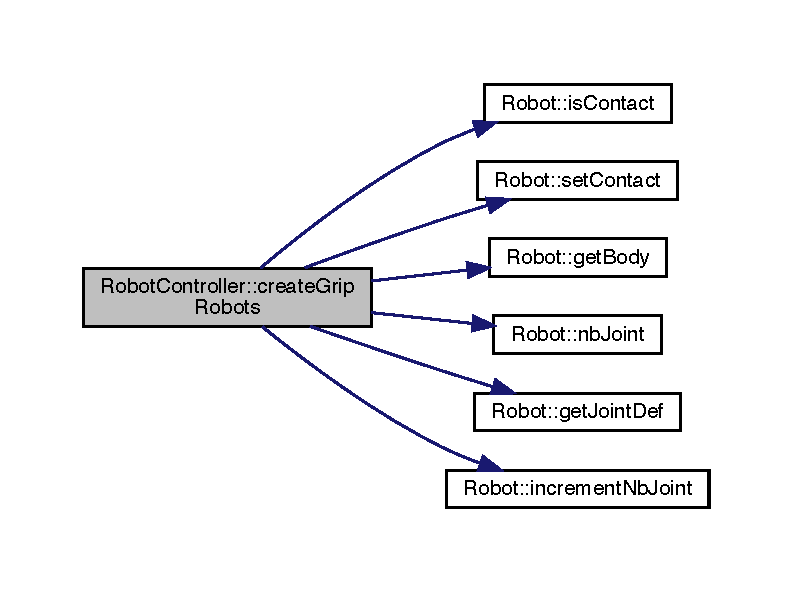
\includegraphics[width=350pt]{class_robot_controller_a6b0bdb7620acbf40f48426e30ff0b759_cgraph}
\end{center}
\end{figure}
Here is the caller graph for this function\+:\nopagebreak
\begin{figure}[H]
\begin{center}
\leavevmode
\includegraphics[width=350pt]{class_robot_controller_a6b0bdb7620acbf40f48426e30ff0b759_icgraph}
\end{center}
\end{figure}
\mbox{\Hypertarget{class_robot_controller_ad79af125e28750338e0da1fb35d0b72d}\label{class_robot_controller_ad79af125e28750338e0da1fb35d0b72d}} 
\index{Robot\+Controller@{Robot\+Controller}!create\+Robot@{create\+Robot}}
\index{create\+Robot@{create\+Robot}!Robot\+Controller@{Robot\+Controller}}
\subsubsection{\texorpdfstring{create\+Robot()}{createRobot()}}
{\footnotesize\ttfamily bool Robot\+Controller\+::create\+Robot (\begin{DoxyParamCaption}\item[{b2\+World $\ast$}]{world,  }\item[{int}]{delay,  }\item[{double}]{posX,  }\item[{double}]{posY,  }\item[{double}]{angle = {\ttfamily 0} }\end{DoxyParamCaption})}

The function create a new robot object and add it to the m\+\_\+robot\+Vector 
\begin{DoxyParams}{Parameters}
{\em world} & pointer on the box2D world object \\
\hline
{\em posX} & initial x position of the robot in meters \\
\hline
{\em posY} & initial y position of the robot in meters \\
\hline
{\em angle} & initial angle of the robot in rad \\
\hline
{\em delay} & number of iteration before the robot is able to move for the first time \\
\hline
\end{DoxyParams}
\begin{DoxyReturn}{Returns}
true if the robot has been created and added to m\+\_\+robot\+Vector, false otherwise 
\end{DoxyReturn}
Here is the caller graph for this function\+:\nopagebreak
\begin{figure}[H]
\begin{center}
\leavevmode
\includegraphics[width=350pt]{class_robot_controller_ad79af125e28750338e0da1fb35d0b72d_icgraph}
\end{center}
\end{figure}
\mbox{\Hypertarget{class_robot_controller_a62fac365f203e2f826efb9b7b7e56854}\label{class_robot_controller_a62fac365f203e2f826efb9b7b7e56854}} 
\index{Robot\+Controller@{Robot\+Controller}!destroy\+Joints@{destroy\+Joints}}
\index{destroy\+Joints@{destroy\+Joints}!Robot\+Controller@{Robot\+Controller}}
\subsubsection{\texorpdfstring{destroy\+Joints()}{destroyJoints()}}
{\footnotesize\ttfamily void Robot\+Controller\+::destroy\+Joints (\begin{DoxyParamCaption}\item[{\mbox{\hyperlink{class_robot}{Robot}} \&}]{robot,  }\item[{\mbox{\hyperlink{_robot_8h_afc015eff6557e84151d2e53b94375445}{side}}}]{s }\end{DoxyParamCaption})}

Remove from the world and destroy a given Box2D joint. This joint is one of a robot gripper 
\begin{DoxyParams}{Parameters}
{\em s} & is either L\+E\+FT or R\+I\+G\+HT  \mbox{\hyperlink{class_robot_a35d0d222246bd7084fac5ae5cdf6d3ce}{Robot\+::m\+\_\+previous\+Grip\+Joint}} and Robot\+::m\+\_\+current\+Grip\+Joint \\
\hline
\end{DoxyParams}
Here is the call graph for this function\+:\nopagebreak
\begin{figure}[H]
\begin{center}
\leavevmode
\includegraphics[width=345pt]{class_robot_controller_a62fac365f203e2f826efb9b7b7e56854_cgraph}
\end{center}
\end{figure}
\mbox{\Hypertarget{class_robot_controller_a2d4d4c93aed605c945e7a95876825bdc}\label{class_robot_controller_a2d4d4c93aed605c945e7a95876825bdc}} 
\index{Robot\+Controller@{Robot\+Controller}!draw\+Robots@{draw\+Robots}}
\index{draw\+Robots@{draw\+Robots}!Robot\+Controller@{Robot\+Controller}}
\subsubsection{\texorpdfstring{draw\+Robots()}{drawRobots()}}
{\footnotesize\ttfamily void Robot\+Controller\+::draw\+Robots (\begin{DoxyParamCaption}\item[{sf\+::\+Render\+Window \&}]{window,  }\item[{double}]{m\+\_\+to\+\_\+px }\end{DoxyParamCaption})}

The function draws all the robots of the \mbox{\hyperlink{class_robot}{Robot}} controller on the S\+F\+ML window 
\begin{DoxyParams}{Parameters}
{\em window} & is the S\+F\+ML window \\
\hline
{\em m\+\_\+to\+\_\+px} & is the conversion factor from m to pixels, it is generally obtained via the terrain \\
\hline
\end{DoxyParams}
Here is the caller graph for this function\+:\nopagebreak
\begin{figure}[H]
\begin{center}
\leavevmode
\includegraphics[width=350pt]{class_robot_controller_a2d4d4c93aed605c945e7a95876825bdc_icgraph}
\end{center}
\end{figure}
\mbox{\Hypertarget{class_robot_controller_a11e413a1ac6466f360f46820d28b0f2e}\label{class_robot_controller_a11e413a1ac6466f360f46820d28b0f2e}} 
\index{Robot\+Controller@{Robot\+Controller}!find\+Contact\+Robots@{find\+Contact\+Robots}}
\index{find\+Contact\+Robots@{find\+Contact\+Robots}!Robot\+Controller@{Robot\+Controller}}
\subsubsection{\texorpdfstring{find\+Contact\+Robots()}{findContactRobots()}}
{\footnotesize\ttfamily void Robot\+Controller\+::find\+Contact\+Robots (\begin{DoxyParamCaption}\item[{b2\+Contact $\ast$}]{contact }\end{DoxyParamCaption})}

This is the function used in the contact\+Listener. It determines if a contact must lead to a grip creation, call the \mbox{\hyperlink{class_robot_aed1ba5683c53ac2b7e4a6c3fc7bcadba}{Robot\+::grip\+Side(b2\+Contact$\ast$ contact, b2\+Body$\ast$ other\+Body, double m\+\_\+to\+\_\+px)}} when a grip has to be created 
\begin{DoxyParams}{Parameters}
{\em contact} & is the Box2D contact object  Robot\+::m\+\_\+state for contacted robots  Robot\+::m\+\_\+left\+Grip\+Joint\+Def or Robot\+::m\+\_\+right\+Grip\+Joint\+Def for future gripping robots  Robot\+::m\+\_\+contact for future gripping robots \\
\hline
\end{DoxyParams}
Here is the call graph for this function\+:\nopagebreak
\begin{figure}[H]
\begin{center}
\leavevmode
\includegraphics[width=350pt]{class_robot_controller_a11e413a1ac6466f360f46820d28b0f2e_cgraph}
\end{center}
\end{figure}
\mbox{\Hypertarget{class_robot_controller_a55f55b2b3b9013bdfc28ad11e0318ce8}\label{class_robot_controller_a55f55b2b3b9013bdfc28ad11e0318ce8}} 
\index{Robot\+Controller@{Robot\+Controller}!get\+Dissolution\+Time@{get\+Dissolution\+Time}}
\index{get\+Dissolution\+Time@{get\+Dissolution\+Time}!Robot\+Controller@{Robot\+Controller}}
\subsubsection{\texorpdfstring{get\+Dissolution\+Time()}{getDissolutionTime()}}
{\footnotesize\ttfamily double Robot\+Controller\+::get\+Dissolution\+Time (\begin{DoxyParamCaption}{ }\end{DoxyParamCaption})}

Get the time required to obtain the dissolution of the bridge. The dissolution is reached when no more robots are in the bridge state \begin{DoxyReturn}{Returns}
the simulated time to reach the dissolution 
\end{DoxyReturn}
\mbox{\Hypertarget{class_robot_controller_a45a4e25b2bb49bf2f1dc18b0f21a6f8d}\label{class_robot_controller_a45a4e25b2bb49bf2f1dc18b0f21a6f8d}} 
\index{Robot\+Controller@{Robot\+Controller}!get\+Nb\+Active\+Robots@{get\+Nb\+Active\+Robots}}
\index{get\+Nb\+Active\+Robots@{get\+Nb\+Active\+Robots}!Robot\+Controller@{Robot\+Controller}}
\subsubsection{\texorpdfstring{get\+Nb\+Active\+Robots()}{getNbActiveRobots()}}
{\footnotesize\ttfamily int Robot\+Controller\+::get\+Nb\+Active\+Robots (\begin{DoxyParamCaption}{ }\end{DoxyParamCaption})}

Get the number of active robots of the robot\+Controller. ie the number of robots in the world window \begin{DoxyReturn}{Returns}
the number of active robots 
\end{DoxyReturn}
Here is the caller graph for this function\+:\nopagebreak
\begin{figure}[H]
\begin{center}
\leavevmode
\includegraphics[width=350pt]{class_robot_controller_a45a4e25b2bb49bf2f1dc18b0f21a6f8d_icgraph}
\end{center}
\end{figure}
\mbox{\Hypertarget{class_robot_controller_a612d9355c9638b9f0bb24348647ada45}\label{class_robot_controller_a612d9355c9638b9f0bb24348647ada45}} 
\index{Robot\+Controller@{Robot\+Controller}!get\+Nb\+Robots@{get\+Nb\+Robots}}
\index{get\+Nb\+Robots@{get\+Nb\+Robots}!Robot\+Controller@{Robot\+Controller}}
\subsubsection{\texorpdfstring{get\+Nb\+Robots()}{getNbRobots()}}
{\footnotesize\ttfamily int Robot\+Controller\+::get\+Nb\+Robots (\begin{DoxyParamCaption}\item[{\mbox{\hyperlink{_robot_8h_a74a75e4700f1f71bb89d80765319e57b}{e\+\_\+state}}}]{s }\end{DoxyParamCaption})}

Get the number of robots of the robot\+Controller under a certain state 
\begin{DoxyParams}{Parameters}
{\em s} & is the considered state, can be either B\+R\+I\+D\+GE or W\+A\+LK \\
\hline
\end{DoxyParams}
\begin{DoxyReturn}{Returns}
the number of robot in this given state 
\end{DoxyReturn}
Here is the caller graph for this function\+:\nopagebreak
\begin{figure}[H]
\begin{center}
\leavevmode
\includegraphics[width=350pt]{class_robot_controller_a612d9355c9638b9f0bb24348647ada45_icgraph}
\end{center}
\end{figure}
\mbox{\Hypertarget{class_robot_controller_a83a58bbd6f7fbafb3038ec0cb6271fda}\label{class_robot_controller_a83a58bbd6f7fbafb3038ec0cb6271fda}} 
\index{Robot\+Controller@{Robot\+Controller}!get\+Nb\+Robots\+Blocked@{get\+Nb\+Robots\+Blocked}}
\index{get\+Nb\+Robots\+Blocked@{get\+Nb\+Robots\+Blocked}!Robot\+Controller@{Robot\+Controller}}
\subsubsection{\texorpdfstring{get\+Nb\+Robots\+Blocked()}{getNbRobotsBlocked()}}
{\footnotesize\ttfamily int Robot\+Controller\+::get\+Nb\+Robots\+Blocked (\begin{DoxyParamCaption}{ }\end{DoxyParamCaption})}

Get the number of robot still active at the end of the simulation \begin{DoxyReturn}{Returns}
the number of robots still active at the time of the function call. 
\end{DoxyReturn}
\mbox{\Hypertarget{class_robot_controller_ae421f813b81632c35ec3494717fd0f12}\label{class_robot_controller_ae421f813b81632c35ec3494717fd0f12}} 
\index{Robot\+Controller@{Robot\+Controller}!get\+Robot@{get\+Robot}}
\index{get\+Robot@{get\+Robot}!Robot\+Controller@{Robot\+Controller}}
\subsubsection{\texorpdfstring{get\+Robot()}{getRobot()}}
{\footnotesize\ttfamily \mbox{\hyperlink{class_robot}{Robot}} $\ast$ Robot\+Controller\+::get\+Robot (\begin{DoxyParamCaption}\item[{int}]{pos\+\_\+id }\end{DoxyParamCaption})}


\begin{DoxyParams}{Parameters}
{\em pos\+\_\+id} & the robot position in the m\+\_\+robot\+Vector \mbox{\hyperlink{class_robot}{Robot}} vector containing all the robots belonging to the \mbox{\hyperlink{class_robot_controller}{Robot\+Controller}}. The pos\+\_\+id starts at 0 Be careful pos\+\_\+id does not necessarily match the robot id \\
\hline
\end{DoxyParams}
\begin{DoxyReturn}{Returns}
a pointer on the robot object 
\end{DoxyReturn}
Here is the caller graph for this function\+:\nopagebreak
\begin{figure}[H]
\begin{center}
\leavevmode
\includegraphics[width=350pt]{class_robot_controller_ae421f813b81632c35ec3494717fd0f12_icgraph}
\end{center}
\end{figure}
\mbox{\Hypertarget{class_robot_controller_aa247b8c90ab585358f07a18c891c8b31}\label{class_robot_controller_aa247b8c90ab585358f07a18c891c8b31}} 
\index{Robot\+Controller@{Robot\+Controller}!get\+Robot\+With\+Id@{get\+Robot\+With\+Id}}
\index{get\+Robot\+With\+Id@{get\+Robot\+With\+Id}!Robot\+Controller@{Robot\+Controller}}
\subsubsection{\texorpdfstring{get\+Robot\+With\+Id()}{getRobotWithId()}}
{\footnotesize\ttfamily \mbox{\hyperlink{class_robot}{Robot}} $\ast$ Robot\+Controller\+::get\+Robot\+With\+Id (\begin{DoxyParamCaption}\item[{int}]{id }\end{DoxyParamCaption})}


\begin{DoxyParams}{Parameters}
{\em id} & is the robot unique id Be careful, it does not necessarily match the robot position within the robots\textquotesingle{} vector. @ return a pointer on the robot object \\
\hline
\end{DoxyParams}
Here is the caller graph for this function\+:\nopagebreak
\begin{figure}[H]
\begin{center}
\leavevmode
\includegraphics[width=350pt]{class_robot_controller_aa247b8c90ab585358f07a18c891c8b31_icgraph}
\end{center}
\end{figure}
\mbox{\Hypertarget{class_robot_controller_acd0a73a62eca471d77a42a0c15964b8e}\label{class_robot_controller_acd0a73a62eca471d77a42a0c15964b8e}} 
\index{Robot\+Controller@{Robot\+Controller}!get\+Stabilization\+Time@{get\+Stabilization\+Time}}
\index{get\+Stabilization\+Time@{get\+Stabilization\+Time}!Robot\+Controller@{Robot\+Controller}}
\subsubsection{\texorpdfstring{get\+Stabilization\+Time()}{getStabilizationTime()}}
{\footnotesize\ttfamily double Robot\+Controller\+::get\+Stabilization\+Time (\begin{DoxyParamCaption}{ }\end{DoxyParamCaption})}

Get the time required to obtain a stable bridge. A stable bridge is reached when the stability condition is reached. This condition is expressed as a duration defined by m\+\_\+controller\+Param.\+stability\+\_\+condition during which no more robots enter the bridge state. This duration can be changed in the main file or as a parameter in the simulation launch. \begin{DoxyReturn}{Returns}
the simulated time to reach stability 
\end{DoxyReturn}
\mbox{\Hypertarget{class_robot_controller_a3191cad0cf82d3378aec0512baf2722b}\label{class_robot_controller_a3191cad0cf82d3378aec0512baf2722b}} 
\index{Robot\+Controller@{Robot\+Controller}!invert\+Moving\+Wheel@{invert\+Moving\+Wheel}}
\index{invert\+Moving\+Wheel@{invert\+Moving\+Wheel}!Robot\+Controller@{Robot\+Controller}}
\subsubsection{\texorpdfstring{invert\+Moving\+Wheel()}{invertMovingWheel()}}
{\footnotesize\ttfamily void Robot\+Controller\+::invert\+Moving\+Wheel (\begin{DoxyParamCaption}\item[{\mbox{\hyperlink{class_robot}{Robot}} \&}]{robot }\end{DoxyParamCaption})}

Invert the moving side of the robot 
\begin{DoxyParams}{Parameters}
{\em robot} & is the \mbox{\hyperlink{class_robot}{Robot}} object  Robot\+::m\+\_\+moving\+Side\+: become L\+E\+FT if it was R\+I\+G\+HT and vice versa \\
\hline
\end{DoxyParams}
\mbox{\Hypertarget{class_robot_controller_a5f3c279e0082ea8dbfe03fd32d8e42b5}\label{class_robot_controller_a5f3c279e0082ea8dbfe03fd32d8e42b5}} 
\index{Robot\+Controller@{Robot\+Controller}!is\+Bridge\+Dissolved@{is\+Bridge\+Dissolved}}
\index{is\+Bridge\+Dissolved@{is\+Bridge\+Dissolved}!Robot\+Controller@{Robot\+Controller}}
\subsubsection{\texorpdfstring{is\+Bridge\+Dissolved()}{isBridgeDissolved()}}
{\footnotesize\ttfamily bool Robot\+Controller\+::is\+Bridge\+Dissolved (\begin{DoxyParamCaption}{ }\end{DoxyParamCaption})}

Check if the bridge has been dissolved. We consider that the dissolution is reached if only one robot remains in the simulation. \begin{DoxyReturn}{Returns}
true if the dissolution of the bridge is obtained, false otherwise 
\end{DoxyReturn}
Here is the call graph for this function\+:\nopagebreak
\begin{figure}[H]
\begin{center}
\leavevmode
\includegraphics[width=350pt]{class_robot_controller_a5f3c279e0082ea8dbfe03fd32d8e42b5_cgraph}
\end{center}
\end{figure}
\mbox{\Hypertarget{class_robot_controller_a05233232614480ea30138101f730a329}\label{class_robot_controller_a05233232614480ea30138101f730a329}} 
\index{Robot\+Controller@{Robot\+Controller}!is\+Bridge\+Stable@{is\+Bridge\+Stable}}
\index{is\+Bridge\+Stable@{is\+Bridge\+Stable}!Robot\+Controller@{Robot\+Controller}}
\subsubsection{\texorpdfstring{is\+Bridge\+Stable()}{isBridgeStable()}}
{\footnotesize\ttfamily bool Robot\+Controller\+::is\+Bridge\+Stable (\begin{DoxyParamCaption}{ }\end{DoxyParamCaption})}

Check if a stable bridge has been obtained. To do so, we compare the time the last robot entered the bridge with the stability condition. The time the last robot has been obtained is stocked inside m\+\_\+stable\+Time. m\+\_\+stable\+Time is updated everytime a robot enter the bridge state via a call of the function \mbox{\hyperlink{class_robot_controller_a797837410a2802b5d7399d132924ba2c}{set\+Robot\+State(\+Robot\& robot,  e\+\_\+state robot\+State)}}; \begin{DoxyReturn}{Returns}
true if a stable bridge is obtained, false otherwise 
\end{DoxyReturn}
Here is the caller graph for this function\+:\nopagebreak
\begin{figure}[H]
\begin{center}
\leavevmode
\includegraphics[width=339pt]{class_robot_controller_a05233232614480ea30138101f730a329_icgraph}
\end{center}
\end{figure}
\mbox{\Hypertarget{class_robot_controller_a0774831ed97c92f24d082603e66950b0}\label{class_robot_controller_a0774831ed97c92f24d082603e66950b0}} 
\index{Robot\+Controller@{Robot\+Controller}!remove\+Robot@{remove\+Robot}}
\index{remove\+Robot@{remove\+Robot}!Robot\+Controller@{Robot\+Controller}}
\subsubsection{\texorpdfstring{remove\+Robot()}{removeRobot()}}
{\footnotesize\ttfamily void Robot\+Controller\+::remove\+Robot (\begin{DoxyParamCaption}{ }\end{DoxyParamCaption})}

Remove robots from the controller and call its destructor. The robots that are destroyed using this method are the ones whose id has been copied inside the m\+\_\+robot\+To\+Destroy vector.  at the end all the robots whose id is in the m\+\_\+robot\+To\+Destroy vector are destroyed and this vector is emptied Here is the caller graph for this function\+:\nopagebreak
\begin{figure}[H]
\begin{center}
\leavevmode
\includegraphics[width=350pt]{class_robot_controller_a0774831ed97c92f24d082603e66950b0_icgraph}
\end{center}
\end{figure}
\mbox{\Hypertarget{class_robot_controller_a68972b0f0f2f033ee0d2d2c849fb38c9}\label{class_robot_controller_a68972b0f0f2f033ee0d2d2c849fb38c9}} 
\index{Robot\+Controller@{Robot\+Controller}!robot\+Out@{robot\+Out}}
\index{robot\+Out@{robot\+Out}!Robot\+Controller@{Robot\+Controller}}
\subsubsection{\texorpdfstring{robot\+Out()}{robotOut()}}
{\footnotesize\ttfamily void Robot\+Controller\+::robot\+Out (\begin{DoxyParamCaption}\item[{double}]{end\+\_\+x,  }\item[{int}]{id }\end{DoxyParamCaption})}

Check if a robot with a given unique id is outside the world. If it is the robot id is copied into the m\+\_\+robot\+To\+Destroy vector to be destroyed at the next call of the \mbox{\hyperlink{class_robot_controller_a0774831ed97c92f24d082603e66950b0}{remove\+Robot()}} method 
\begin{DoxyParams}{Parameters}
{\em end\+\_\+x} & corresponds to the end of the world \\
\hline
{\em id} & is the unique id of the robot, can be obtained with robot.\+get\+I\+D() \\
\hline
\end{DoxyParams}
\mbox{\Hypertarget{class_robot_controller_a927abf2765cd53b39acf128f318c3fe5}\label{class_robot_controller_a927abf2765cd53b39acf128f318c3fe5}} 
\index{Robot\+Controller@{Robot\+Controller}!robot\+Pushing@{robot\+Pushing}}
\index{robot\+Pushing@{robot\+Pushing}!Robot\+Controller@{Robot\+Controller}}
\subsubsection{\texorpdfstring{robot\+Pushing()}{robotPushing()}}
{\footnotesize\ttfamily bool Robot\+Controller\+::robot\+Pushing (\begin{DoxyParamCaption}\item[{\mbox{\hyperlink{class_robot}{Robot}} \&}]{r }\end{DoxyParamCaption})}

Determine if a robot is pushing after the pushing delay has been reached by determining if the robot is touching another object. This contact has to be on the moving side. This is checked by calling the function Robot\+::contact\+On\+Grip\+Side(b2\+Contact$\ast$ contact). In addition, the robot must have run a higher angle than m\+\_\+angle\+\_\+min to avoid gripping the exact previous position 
\begin{DoxyParams}{Parameters}
{\em r} & is the \mbox{\hyperlink{class_robot}{Robot}} to be checked when its delay corresponds to the pushing\+\_\+delay, if no direct joint has been created  Robot\+::m\+\_\+delay, Robot\+::m\+\_\+contact, Robot\+::m\+\_\+left\+Grip\+Joint\+Def, Robot\+::m\+\_\+right\+Grip\+Joint\+Def \\
\hline
\end{DoxyParams}
\begin{DoxyReturn}{Returns}
true if the robot is pushing, false otherwise 
\end{DoxyReturn}
Here is the call graph for this function\+:\nopagebreak
\begin{figure}[H]
\begin{center}
\leavevmode
\includegraphics[width=350pt]{class_robot_controller_a927abf2765cd53b39acf128f318c3fe5_cgraph}
\end{center}
\end{figure}
\mbox{\Hypertarget{class_robot_controller_a83d343eb8958d365624d06ac1b0b1b3d}\label{class_robot_controller_a83d343eb8958d365624d06ac1b0b1b3d}} 
\index{Robot\+Controller@{Robot\+Controller}!robot\+Stacking@{robot\+Stacking}}
\index{robot\+Stacking@{robot\+Stacking}!Robot\+Controller@{Robot\+Controller}}
\subsubsection{\texorpdfstring{robot\+Stacking()}{robotStacking()}}
{\footnotesize\ttfamily bool Robot\+Controller\+::robot\+Stacking (\begin{DoxyParamCaption}\item[{\mbox{\hyperlink{class_robot}{Robot}} $\ast$}]{r,  }\item[{float}]{posX }\end{DoxyParamCaption})}

This function is used to help determine if the robots are stacking. It is called when a new robot will be created to check if the previous robot is too close to the new robot. The previous robot is too close when it is located before the given position posX + one body\+Length unit. 
\begin{DoxyParams}{Parameters}
{\em r} & is the \mbox{\hyperlink{class_robot}{Robot}} to be checked \\
\hline
{\em posX} & is the superior limit of the position one wants to check \\
\hline
\end{DoxyParams}
\begin{DoxyReturn}{Returns}
true if the robot is located before posX, false otherwise 
\end{DoxyReturn}
Here is the call graph for this function\+:\nopagebreak
\begin{figure}[H]
\begin{center}
\leavevmode
\includegraphics[width=350pt]{class_robot_controller_a83d343eb8958d365624d06ac1b0b1b3d_cgraph}
\end{center}
\end{figure}
Here is the caller graph for this function\+:\nopagebreak
\begin{figure}[H]
\begin{center}
\leavevmode
\includegraphics[width=350pt]{class_robot_controller_a83d343eb8958d365624d06ac1b0b1b3d_icgraph}
\end{center}
\end{figure}
\mbox{\Hypertarget{class_robot_controller_a19191b156161bd7a3978659329ceaad2}\label{class_robot_controller_a19191b156161bd7a3978659329ceaad2}} 
\index{Robot\+Controller@{Robot\+Controller}!set\+Bridge\+Stability@{set\+Bridge\+Stability}}
\index{set\+Bridge\+Stability@{set\+Bridge\+Stability}!Robot\+Controller@{Robot\+Controller}}
\subsubsection{\texorpdfstring{set\+Bridge\+Stability()}{setBridgeStability()}}
{\footnotesize\ttfamily void Robot\+Controller\+::set\+Bridge\+Stability (\begin{DoxyParamCaption}\item[{bool}]{stable }\end{DoxyParamCaption})}

Change the bridge stability flag value. 
\begin{DoxyParams}{Parameters}
{\em stable} & is either true if the stability has been reached or false  m\+\_\+is\+Stable \\
\hline
\end{DoxyParams}
Here is the caller graph for this function\+:\nopagebreak
\begin{figure}[H]
\begin{center}
\leavevmode
\includegraphics[width=350pt]{class_robot_controller_a19191b156161bd7a3978659329ceaad2_icgraph}
\end{center}
\end{figure}
\mbox{\Hypertarget{class_robot_controller_adf00a753bc750624e805f57f8998ad78}\label{class_robot_controller_adf00a753bc750624e805f57f8998ad78}} 
\index{Robot\+Controller@{Robot\+Controller}!set\+Nb\+Robots@{set\+Nb\+Robots}}
\index{set\+Nb\+Robots@{set\+Nb\+Robots}!Robot\+Controller@{Robot\+Controller}}
\subsubsection{\texorpdfstring{set\+Nb\+Robots()}{setNbRobots()}}
{\footnotesize\ttfamily void Robot\+Controller\+::set\+Nb\+Robots (\begin{DoxyParamCaption}\item[{int}]{nb\+\_\+robots }\end{DoxyParamCaption})}

Set the maximum number of robots that can be active at the same time in the simulation window. It is used to limit the size of the m\+\_\+robot\+Vector. 
\begin{DoxyParams}{Parameters}
{\em nb\+\_\+robots} & is the maximum number of robot that can be existing at the same time. \\
\hline
\end{DoxyParams}
\mbox{\Hypertarget{class_robot_controller_a797837410a2802b5d7399d132924ba2c}\label{class_robot_controller_a797837410a2802b5d7399d132924ba2c}} 
\index{Robot\+Controller@{Robot\+Controller}!set\+Robot\+State@{set\+Robot\+State}}
\index{set\+Robot\+State@{set\+Robot\+State}!Robot\+Controller@{Robot\+Controller}}
\subsubsection{\texorpdfstring{set\+Robot\+State()}{setRobotState()}}
{\footnotesize\ttfamily void Robot\+Controller\+::set\+Robot\+State (\begin{DoxyParamCaption}\item[{\mbox{\hyperlink{class_robot}{Robot}} \&}]{robot,  }\item[{\mbox{\hyperlink{_robot_8h_a74a75e4700f1f71bb89d80765319e57b}{e\+\_\+state}}}]{robot\+State }\end{DoxyParamCaption})}

Function used to set the state of a specific robot 
\begin{DoxyParams}{Parameters}
{\em robot} & is the \mbox{\hyperlink{class_robot}{Robot}} object \\
\hline
{\em robot\+State} & can be either W\+A\+LK or B\+R\+I\+D\+GE  Robot\+::m\+\_\+moving, Robot\+::m\+\_\+state, Robot\+::m\+\_\+contact and Robot\+::m\+\_\+delay \\
\hline
\end{DoxyParams}
Here is the caller graph for this function\+:\nopagebreak
\begin{figure}[H]
\begin{center}
\leavevmode
\includegraphics[width=350pt]{class_robot_controller_a797837410a2802b5d7399d132924ba2c_icgraph}
\end{center}
\end{figure}
\mbox{\Hypertarget{class_robot_controller_a76d6bb1e93bb9523850370fdf76407c4}\label{class_robot_controller_a76d6bb1e93bb9523850370fdf76407c4}} 
\index{Robot\+Controller@{Robot\+Controller}!set\+Scale@{set\+Scale}}
\index{set\+Scale@{set\+Scale}!Robot\+Controller@{Robot\+Controller}}
\subsubsection{\texorpdfstring{set\+Scale()}{setScale()}}
{\footnotesize\ttfamily void Robot\+Controller\+::set\+Scale (\begin{DoxyParamCaption}\item[{double}]{m\+\_\+to\+\_\+px }\end{DoxyParamCaption})}

Set the scale to do the conversion from real dimensions (m) to simulated ones (pixels). Ususlly the scale is obtained from the terrain with the \mbox{\hyperlink{class_terrain_af0cff27a194359a13c448c89bd374de3}{Terrain\+::get\+Scale()}} method. 
\begin{DoxyParams}{Parameters}
{\em m\+\_\+to\+\_\+px} & is the conversion factor from meters to pixels \\
\hline
\end{DoxyParams}
\mbox{\Hypertarget{class_robot_controller_ab2e4091fc2e47701cc5dbd7c2d9fc649}\label{class_robot_controller_ab2e4091fc2e47701cc5dbd7c2d9fc649}} 
\index{Robot\+Controller@{Robot\+Controller}!step@{step}}
\index{step@{step}!Robot\+Controller@{Robot\+Controller}}
\subsubsection{\texorpdfstring{step()}{step()}}
{\footnotesize\ttfamily void Robot\+Controller\+::step (\begin{DoxyParamCaption}\item[{double}]{end\+\_\+x }\end{DoxyParamCaption})}

Run a step of the simulation. 
\begin{DoxyParams}{Parameters}
{\em end\+\_\+x} & is the position of the end of the simulation world it generally correspond to the end of the window. above this position the robot is destroyed. \\
\hline
\end{DoxyParams}
Here is the call graph for this function\+:\nopagebreak
\begin{figure}[H]
\begin{center}
\leavevmode
\includegraphics[width=350pt]{class_robot_controller_ab2e4091fc2e47701cc5dbd7c2d9fc649_cgraph}
\end{center}
\end{figure}
Here is the caller graph for this function\+:\nopagebreak
\begin{figure}[H]
\begin{center}
\leavevmode
\includegraphics[width=322pt]{class_robot_controller_ab2e4091fc2e47701cc5dbd7c2d9fc649_icgraph}
\end{center}
\end{figure}
\mbox{\Hypertarget{class_robot_controller_ae433d7a77a59e8eced35fc4885051805}\label{class_robot_controller_ae433d7a77a59e8eced35fc4885051805}} 
\index{Robot\+Controller@{Robot\+Controller}!wait\+\_\+delay@{wait\+\_\+delay}}
\index{wait\+\_\+delay@{wait\+\_\+delay}!Robot\+Controller@{Robot\+Controller}}
\subsubsection{\texorpdfstring{wait\+\_\+delay()}{wait\_delay()}}
{\footnotesize\ttfamily void Robot\+Controller\+::wait\+\_\+delay (\begin{DoxyParamCaption}\item[{\mbox{\hyperlink{class_robot}{Robot}} \&}]{robot }\end{DoxyParamCaption})}

Handle the waiting delay of the robots by decreasing it at each world step. When the delay is null, the robot.\+m\+\_\+ready state is set to true 
\begin{DoxyParams}{Parameters}
{\em robot} & generally from the m\+\_\+robot\+Vector of the controller  Robot\+::m\+\_\+ready is set to true when Robot\+::m\+\_\+delay is null  Robot\+::m\+\_\+delay is decreased otherwise \\
\hline
\end{DoxyParams}
Here is the call graph for this function\+:\nopagebreak
\begin{figure}[H]
\begin{center}
\leavevmode
\includegraphics[width=313pt]{class_robot_controller_ae433d7a77a59e8eced35fc4885051805_cgraph}
\end{center}
\end{figure}
Here is the caller graph for this function\+:\nopagebreak
\begin{figure}[H]
\begin{center}
\leavevmode
\includegraphics[width=350pt]{class_robot_controller_ae433d7a77a59e8eced35fc4885051805_icgraph}
\end{center}
\end{figure}


\subsection{Member Data Documentation}
\mbox{\Hypertarget{class_robot_controller_abe09204acb8936eddcacbae0b023423a}\label{class_robot_controller_abe09204acb8936eddcacbae0b023423a}} 
\index{Robot\+Controller@{Robot\+Controller}!m\+\_\+bridge\+Entry@{m\+\_\+bridge\+Entry}}
\index{m\+\_\+bridge\+Entry@{m\+\_\+bridge\+Entry}!Robot\+Controller@{Robot\+Controller}}
\subsubsection{\texorpdfstring{m\+\_\+bridge\+Entry}{m\_bridgeEntry}}
{\footnotesize\ttfamily bool Robot\+Controller\+::m\+\_\+bridge\+Entry = false}

Flag used to notify when a new robot enter the bridge state. It is used to write a new entry in the bridge file. It is set to false once the bridge file have been updated (in the demo.\+cpp file). 

The documentation for this class was generated from the following files\+:\begin{DoxyCompactItemize}
\item 
simulation/src/\mbox{\hyperlink{_robot_controller_8h}{Robot\+Controller.\+h}}\item 
simulation/src/Robot\+Controller.\+cpp\end{DoxyCompactItemize}

\hypertarget{structconfig_1_1s_config}{}\section{config\+:\+:s\+Config Struct Reference}
\label{structconfig_1_1s_config}\index{config\+::s\+Config@{config\+::s\+Config}}


Collaboration diagram for config\+:\+:s\+Config\+:\nopagebreak
\begin{figure}[H]
\begin{center}
\leavevmode
\includegraphics[width=346pt]{structconfig_1_1s_config__coll__graph}
\end{center}
\end{figure}
\subsection*{Public Attributes}
\begin{DoxyCompactItemize}
\item 
\mbox{\Hypertarget{structconfig_1_1s_config_aca277421f902bb9f2c25b9428a9957b3}\label{structconfig_1_1s_config_aca277421f902bb9f2c25b9428a9957b3}} 
struct \mbox{\hyperlink{structconfig_1_1s_terrain}{s\+Terrain}} {\bfseries terrain}
\item 
\mbox{\Hypertarget{structconfig_1_1s_config_a057b9b1fa05fb7b024ff6c20ab93e5e2}\label{structconfig_1_1s_config_a057b9b1fa05fb7b024ff6c20ab93e5e2}} 
struct \mbox{\hyperlink{structconfig_1_1s_simulation}{s\+Simulation}} {\bfseries simulation}
\item 
\mbox{\Hypertarget{structconfig_1_1s_config_af6a5e9f0eb966ad92a2fd7428d5ee17e}\label{structconfig_1_1s_config_af6a5e9f0eb966ad92a2fd7428d5ee17e}} 
struct \mbox{\hyperlink{structconfig_1_1s_controller}{s\+Controller}} {\bfseries controller}
\item 
\mbox{\Hypertarget{structconfig_1_1s_config_aa02aeb8d778bbe36900505ea0b844404}\label{structconfig_1_1s_config_aa02aeb8d778bbe36900505ea0b844404}} 
struct \mbox{\hyperlink{structconfig_1_1s_robot}{s\+Robot}} {\bfseries robot}
\item 
\mbox{\Hypertarget{structconfig_1_1s_config_a397d5923dd1cb6a1cf49df3d62872a98}\label{structconfig_1_1s_config_a397d5923dd1cb6a1cf49df3d62872a98}} 
struct \mbox{\hyperlink{structconfig_1_1s_window}{s\+Window}} {\bfseries window}
\item 
\mbox{\Hypertarget{structconfig_1_1s_config_a92296b4802c10df4be246afb182b34ba}\label{structconfig_1_1s_config_a92296b4802c10df4be246afb182b34ba}} 
std\+::string {\bfseries logfile\+\_\+name}
\item 
\mbox{\Hypertarget{structconfig_1_1s_config_a140ad96bb800b9a2316e1c726a033c36}\label{structconfig_1_1s_config_a140ad96bb800b9a2316e1c726a033c36}} 
std\+::string {\bfseries logfile\+\_\+path}
\end{DoxyCompactItemize}


The documentation for this struct was generated from the following file\+:\begin{DoxyCompactItemize}
\item 
simulation/src/\mbox{\hyperlink{_config_8h}{Config.\+h}}\end{DoxyCompactItemize}

\hypertarget{structconfig_1_1s_controller}{}\section{config\+:\+:s\+Controller Struct Reference}
\label{structconfig_1_1s_controller}\index{config\+::s\+Controller@{config\+::s\+Controller}}
\subsection*{Public Attributes}
\begin{DoxyCompactItemize}
\item 
\mbox{\Hypertarget{structconfig_1_1s_controller_a8923acd9bfb67b8e9e3c1c3c8dbec683}\label{structconfig_1_1s_controller_a8923acd9bfb67b8e9e3c1c3c8dbec683}} 
double {\bfseries angle\+\_\+limit}
\item 
\mbox{\Hypertarget{structconfig_1_1s_controller_a2fde08fbf75929ab52e5e23cee7cc221}\label{structconfig_1_1s_controller_a2fde08fbf75929ab52e5e23cee7cc221}} 
double {\bfseries bridge\+\_\+delay}
\item 
\mbox{\Hypertarget{structconfig_1_1s_controller_ae6375847a7a00925fb89b9410b37ce1f}\label{structconfig_1_1s_controller_ae6375847a7a00925fb89b9410b37ce1f}} 
double {\bfseries walk\+\_\+delay}
\item 
\mbox{\Hypertarget{structconfig_1_1s_controller_af54d74a54e118e607b93f0cda27d4898}\label{structconfig_1_1s_controller_af54d74a54e118e607b93f0cda27d4898}} 
double {\bfseries time\+\_\+before\+\_\+pushing}
\item 
\mbox{\Hypertarget{structconfig_1_1s_controller_a945185f0421baea5a8d447e75ec78b38}\label{structconfig_1_1s_controller_a945185f0421baea5a8d447e75ec78b38}} 
int {\bfseries max\+\_\+robot\+\_\+window}
\item 
\mbox{\Hypertarget{structconfig_1_1s_controller_ad6caeeebb6d554e790a62a3d6939d853}\label{structconfig_1_1s_controller_ad6caeeebb6d554e790a62a3d6939d853}} 
double {\bfseries stability\+\_\+condition}
\end{DoxyCompactItemize}


The documentation for this struct was generated from the following file\+:\begin{DoxyCompactItemize}
\item 
simulation/src/\mbox{\hyperlink{_config_8h}{Config.\+h}}\end{DoxyCompactItemize}

\hypertarget{structconfig_1_1s_robot}{}\section{config\+:\+:s\+Robot Struct Reference}
\label{structconfig_1_1s_robot}\index{config\+::s\+Robot@{config\+::s\+Robot}}
\subsection*{Public Attributes}
\begin{DoxyCompactItemize}
\item 
\mbox{\Hypertarget{structconfig_1_1s_robot_a825d14248f65e3eeeb159c2cb54ab3cb}\label{structconfig_1_1s_robot_a825d14248f65e3eeeb159c2cb54ab3cb}} 
double {\bfseries body\+\_\+length}
\item 
\mbox{\Hypertarget{structconfig_1_1s_robot_ab3ed79becfa66c518fcef7583b8a5179}\label{structconfig_1_1s_robot_ab3ed79becfa66c518fcef7583b8a5179}} 
double {\bfseries speed}
\item 
\mbox{\Hypertarget{structconfig_1_1s_robot_a4a22c395cc9d20e8c3e424129bb5ccc6}\label{structconfig_1_1s_robot_a4a22c395cc9d20e8c3e424129bb5ccc6}} 
double {\bfseries wheel\+\_\+distance}
\item 
\mbox{\Hypertarget{structconfig_1_1s_robot_a2b7da73a6f21f32ee3ab0262e804f889}\label{structconfig_1_1s_robot_a2b7da73a6f21f32ee3ab0262e804f889}} 
double {\bfseries attach\+\_\+height}
\item 
\mbox{\Hypertarget{structconfig_1_1s_robot_a097bf4c624355c380b64216da30514ec}\label{structconfig_1_1s_robot_a097bf4c624355c380b64216da30514ec}} 
double {\bfseries wheel\+\_\+radius}
\end{DoxyCompactItemize}


The documentation for this struct was generated from the following file\+:\begin{DoxyCompactItemize}
\item 
simulation/src/\mbox{\hyperlink{_config_8h}{Config.\+h}}\end{DoxyCompactItemize}

\hypertarget{structconfig_1_1s_simulation}{}\section{config\+:\+:s\+Simulation Struct Reference}
\label{structconfig_1_1s_simulation}\index{config\+::s\+Simulation@{config\+::s\+Simulation}}
\subsection*{Public Attributes}
\begin{DoxyCompactItemize}
\item 
\mbox{\Hypertarget{structconfig_1_1s_simulation_a25ccff214dabfb1a6f711f8350ae8871}\label{structconfig_1_1s_simulation_a25ccff214dabfb1a6f711f8350ae8871}} 
double {\bfseries gravity}
\item 
\mbox{\Hypertarget{structconfig_1_1s_simulation_a967cb0f1917b6a79271401bf64978533}\label{structconfig_1_1s_simulation_a967cb0f1917b6a79271401bf64978533}} 
double {\bfseries robot\+\_\+delay}
\item 
\mbox{\Hypertarget{structconfig_1_1s_simulation_a9a76eabe85007447b4ffc3cf80499661}\label{structconfig_1_1s_simulation_a9a76eabe85007447b4ffc3cf80499661}} 
double {\bfseries robot\+\_\+distance}
\item 
\mbox{\Hypertarget{structconfig_1_1s_simulation_a162430ba1e14142b5e17c46607473a5d}\label{structconfig_1_1s_simulation_a162430ba1e14142b5e17c46607473a5d}} 
double {\bfseries robot\+\_\+phase}
\item 
\mbox{\Hypertarget{structconfig_1_1s_simulation_a79abcea43cc4f6b0288b89ef25cc0001}\label{structconfig_1_1s_simulation_a79abcea43cc4f6b0288b89ef25cc0001}} 
double {\bfseries robot\+\_\+initial\+\_\+posX}
\item 
\mbox{\Hypertarget{structconfig_1_1s_simulation_a5f210266729c02d90c6434407c520a46}\label{structconfig_1_1s_simulation_a5f210266729c02d90c6434407c520a46}} 
double {\bfseries robot\+\_\+initial\+\_\+posY}
\item 
\mbox{\Hypertarget{structconfig_1_1s_simulation_a2c1ada081a51c0fe22a0a792e86b2a7d}\label{structconfig_1_1s_simulation_a2c1ada081a51c0fe22a0a792e86b2a7d}} 
int {\bfseries nb\+\_\+robots}
\item 
\mbox{\Hypertarget{structconfig_1_1s_simulation_aff5f4baa8b4f27a11ddb1ca2dae35aee}\label{structconfig_1_1s_simulation_aff5f4baa8b4f27a11ddb1ca2dae35aee}} 
double {\bfseries bridge\+\_\+duration}
\item 
\mbox{\Hypertarget{structconfig_1_1s_simulation_ad8704f9eb529596937a9ab05f776f8ea}\label{structconfig_1_1s_simulation_ad8704f9eb529596937a9ab05f776f8ea}} 
double {\bfseries dissolution\+\_\+duration}
\item 
\mbox{\Hypertarget{structconfig_1_1s_simulation_a4e43c8d5ae20bd2e8bd9b3465a974de7}\label{structconfig_1_1s_simulation_a4e43c8d5ae20bd2e8bd9b3465a974de7}} 
bool {\bfseries visualization}
\end{DoxyCompactItemize}


The documentation for this struct was generated from the following file\+:\begin{DoxyCompactItemize}
\item 
simulation/src/Config.\+h\end{DoxyCompactItemize}

\hypertarget{structconfig_1_1s_terrain}{}\section{config\+:\+:s\+Terrain Struct Reference}
\label{structconfig_1_1s_terrain}\index{config\+::s\+Terrain@{config\+::s\+Terrain}}
\subsection*{Public Attributes}
\begin{DoxyCompactItemize}
\item 
double \mbox{\hyperlink{structconfig_1_1s_terrain_ad6c30d8e675a81113ff3e5af46e636ac}{runaway}}
\item 
\mbox{\Hypertarget{structconfig_1_1s_terrain_a6a8545cc6a2c5a232f5e60971a92cbb0}\label{structconfig_1_1s_terrain_a6a8545cc6a2c5a232f5e60971a92cbb0}} 
double {\bfseries v\+\_\+width}
\item 
\mbox{\Hypertarget{structconfig_1_1s_terrain_aee6358b6e85e5599aa76af2e0f765ca0}\label{structconfig_1_1s_terrain_aee6358b6e85e5599aa76af2e0f765ca0}} 
double {\bfseries v\+\_\+height}
\item 
\mbox{\Hypertarget{structconfig_1_1s_terrain_a8e98646a0b5acab7df066a6859459b2e}\label{structconfig_1_1s_terrain_a8e98646a0b5acab7df066a6859459b2e}} 
double {\bfseries v\+\_\+angle}
\end{DoxyCompactItemize}


\subsection{Member Data Documentation}
\mbox{\Hypertarget{structconfig_1_1s_terrain_ad6c30d8e675a81113ff3e5af46e636ac}\label{structconfig_1_1s_terrain_ad6c30d8e675a81113ff3e5af46e636ac}} 
\index{config\+::s\+Terrain@{config\+::s\+Terrain}!runaway@{runaway}}
\index{runaway@{runaway}!config\+::s\+Terrain@{config\+::s\+Terrain}}
\subsubsection{\texorpdfstring{runaway}{runaway}}
{\footnotesize\ttfamily double config\+::s\+Terrain\+::runaway}

It is either the distance before the eentrance of the obstcle or 1/3 of the length of the ground in the default terrain 

The documentation for this struct was generated from the following file\+:\begin{DoxyCompactItemize}
\item 
simulation/src/\mbox{\hyperlink{_config_8h}{Config.\+h}}\end{DoxyCompactItemize}

\hypertarget{structconfig_1_1s_window}{}\section{config\+:\+:s\+Window Struct Reference}
\label{structconfig_1_1s_window}\index{config\+::s\+Window@{config\+::s\+Window}}
\subsection*{Public Attributes}
\begin{DoxyCompactItemize}
\item 
\mbox{\Hypertarget{structconfig_1_1s_window_aed552708ff733ec85593fd96113552e0}\label{structconfig_1_1s_window_aed552708ff733ec85593fd96113552e0}} 
int {\bfseries W\+I\+N\+D\+O\+W\+\_\+\+X\+\_\+\+PX}
\item 
\mbox{\Hypertarget{structconfig_1_1s_window_ad61587d1e8b181ead0b2bd6b60f81dec}\label{structconfig_1_1s_window_ad61587d1e8b181ead0b2bd6b60f81dec}} 
int {\bfseries W\+I\+N\+D\+O\+W\+\_\+\+Y\+\_\+\+PX}
\end{DoxyCompactItemize}


The documentation for this struct was generated from the following file\+:\begin{DoxyCompactItemize}
\item 
simulation/src/\mbox{\hyperlink{_config_8h}{Config.\+h}}\end{DoxyCompactItemize}

\hypertarget{class_terrain}{}\section{Terrain Class Reference}
\label{class_terrain}\index{Terrain@{Terrain}}


Inheritance diagram for Terrain\+:\nopagebreak
\begin{figure}[H]
\begin{center}
\leavevmode
\includegraphics[width=350pt]{class_terrain__inherit__graph}
\end{center}
\end{figure}


Collaboration diagram for Terrain\+:\nopagebreak
\begin{figure}[H]
\begin{center}
\leavevmode
\includegraphics[width=196pt]{class_terrain__coll__graph}
\end{center}
\end{figure}
\subsection*{Public Member Functions}
\begin{DoxyCompactItemize}
\item 
\mbox{\Hypertarget{class_terrain_ae0f4cfd17060701ae6bf4e14e126ef5e}\label{class_terrain_ae0f4cfd17060701ae6bf4e14e126ef5e}} 
{\bfseries Terrain} (b2\+World $\ast$world, sf\+::\+Render\+Window \&window, \mbox{\hyperlink{structconfig_1_1s_terrain}{config\+::s\+Terrain}} terrain\+Param, int W\+I\+N\+D\+O\+W\+\_\+\+X\+\_\+\+PX, double body\+Length=1)
\item 
virtual void \mbox{\hyperlink{class_terrain_ae7515dee9afa3b1cefac459abefb5442}{create}} (b2\+World $\ast$world, sf\+::\+Render\+Window \&window, \mbox{\hyperlink{structconfig_1_1s_terrain}{config\+::s\+Terrain}} terrain\+Param, int W\+I\+N\+D\+O\+W\+\_\+\+X\+\_\+\+PX, double body\+Length)
\item 
virtual void \mbox{\hyperlink{class_terrain_a97e007277f8abb9dde20ef2b49c38a3a}{create\+Body}} (b2\+World $\ast$world)
\item 
virtual void \mbox{\hyperlink{class_terrain_ae60571b91c1979fa94bdfc5002da6ac7}{draw\+Body}} (sf\+::\+Render\+Window \&window)
\item 
virtual \mbox{\hyperlink{_terrain_8h_a6d0b7e83bb7325270c1162bece970fd8}{e\+\_\+terrain\+\_\+type}} \mbox{\hyperlink{class_terrain_a6cd1220b8e64466cc7a2219efff4141b}{get\+Type}} ()
\item 
virtual b2\+Vec2 \mbox{\hyperlink{class_terrain_a8a8629396e5cb03961649acdc23eacf2}{get\+Top\+Left\+Corner}} ()
\item 
virtual b2\+Vec2 \mbox{\hyperlink{class_terrain_a10fcf414cba83e769d99156fe16aa795}{get\+Top\+Right\+Corner}} ()
\item 
virtual b2\+Vec2 \mbox{\hyperlink{class_terrain_a26e1c7c05b8256015730df34d97d29c2}{get\+Bottom}} ()
\item 
double \mbox{\hyperlink{class_terrain_a819253da1f67d199b6347b93071961e7}{get\+V\+Length}} ()
\item 
b2\+Body $\ast$ \mbox{\hyperlink{class_terrain_aa0e70c6bbd39935c69c2b6edb74fcd32}{get\+Body}} ()
\item 
const double \mbox{\hyperlink{class_terrain_af0cff27a194359a13c448c89bd374de3}{get\+Scale}} ()
\end{DoxyCompactItemize}
\subsection*{Protected Attributes}
\begin{DoxyCompactItemize}
\item 
\mbox{\Hypertarget{class_terrain_a4b1a5b1e598de229ea88bdef21ee7fbc}\label{class_terrain_a4b1a5b1e598de229ea88bdef21ee7fbc}} 
b2\+Body $\ast$ {\bfseries m\+\_\+ground\+Body}
\item 
\mbox{\Hypertarget{class_terrain_a92f36542edc1a5662bb07e6b7e459e56}\label{class_terrain_a92f36542edc1a5662bb07e6b7e459e56}} 
double {\bfseries m\+\_\+body\+Length}
\item 
\mbox{\Hypertarget{class_terrain_ab4ad9370a342c622416df70bdcd1d1b6}\label{class_terrain_ab4ad9370a342c622416df70bdcd1d1b6}} 
double {\bfseries m\+\_\+\+M\+\_\+\+T\+O\+\_\+\+PX}
\item 
\mbox{\Hypertarget{class_terrain_aa41ca0c300d1f82566a6a3e78380b284}\label{class_terrain_aa41ca0c300d1f82566a6a3e78380b284}} 
double {\bfseries m\+\_\+width}
\item 
\mbox{\Hypertarget{class_terrain_ab86d8eee1847a2c9bf048c7ddcb5d121}\label{class_terrain_ab86d8eee1847a2c9bf048c7ddcb5d121}} 
double {\bfseries m\+\_\+height}
\item 
\mbox{\Hypertarget{class_terrain_a9d8af4fbe1c713f6e582562465ec15f7}\label{class_terrain_a9d8af4fbe1c713f6e582562465ec15f7}} 
double {\bfseries m\+\_\+runaway}
\item 
\mbox{\Hypertarget{class_terrain_a3f3d3c1f5d75f1920d82ca36a9cc086b}\label{class_terrain_a3f3d3c1f5d75f1920d82ca36a9cc086b}} 
double {\bfseries m\+\_\+angle}
\item 
\mbox{\Hypertarget{class_terrain_a03ab57eab744c95cc368646acb94ae7b}\label{class_terrain_a03ab57eab744c95cc368646acb94ae7b}} 
double {\bfseries m\+\_\+posY} =2.\+5
\item 
\mbox{\Hypertarget{class_terrain_a8d3792a6911e30eb4ca67c5efd1002df}\label{class_terrain_a8d3792a6911e30eb4ca67c5efd1002df}} 
\mbox{\hyperlink{structconfig_1_1s_terrain}{config\+::s\+Terrain}} {\bfseries m\+\_\+terrain\+Param}
\end{DoxyCompactItemize}


\subsection{Member Function Documentation}
\mbox{\Hypertarget{class_terrain_ae7515dee9afa3b1cefac459abefb5442}\label{class_terrain_ae7515dee9afa3b1cefac459abefb5442}} 
\index{Terrain@{Terrain}!create@{create}}
\index{create@{create}!Terrain@{Terrain}}
\subsubsection{\texorpdfstring{create()}{create()}}
{\footnotesize\ttfamily void Terrain\+::create (\begin{DoxyParamCaption}\item[{b2\+World $\ast$}]{world,  }\item[{sf\+::\+Render\+Window \&}]{window,  }\item[{\mbox{\hyperlink{structconfig_1_1s_terrain}{config\+::s\+Terrain}}}]{terrain\+Param,  }\item[{int}]{W\+I\+N\+D\+O\+W\+\_\+\+X\+\_\+\+PX,  }\item[{double}]{body\+Length }\end{DoxyParamCaption})\hspace{0.3cm}{\ttfamily [virtual]}}

The function create M\+U\+ST be called if the terrain object has been created via the default constructor (ex when created dynamically with new), otherwise no need to use it 
\begin{DoxyParams}{Parameters}
{\em world} & is a pointer on the Box2D world object \\
\hline
{\em window} & is the S\+F\+ML window \\
\hline
{\em terrain\+Param} & are the terrain parameters (cf \mbox{\hyperlink{_config_8h}{Config.\+h}}) \\
\hline
{\em W\+I\+N\+D\+O\+W\+\_\+\+X\+\_\+\+PX} & is the x-\/size of the window. it is used to calculate the scale to convert from meters to pixels \\
\hline
{\em bodylength} & is the size of a robot. it is used to convert the dimension from body length to m \\
\hline
\end{DoxyParams}


Reimplemented in \mbox{\hyperlink{class_ramp_a0dcb7d44807cb9ce61307c975b29f06e}{Ramp}}, \mbox{\hyperlink{class_v2_b_l_terrain_ad9b52b119e46602caa16ec4bfbb3966a}{V2\+B\+L\+Terrain}}, \mbox{\hyperlink{class_vterrain_a480ed9dbd18d1806fa68f44857f3cf99}{Vterrain}}, \mbox{\hyperlink{class_box_terrain_a175fb845b46ed36cd0b4516b4bb64fb3}{Box\+Terrain}}, and \mbox{\hyperlink{class_v_stepper_adc0daf55fe95e9059576ae432bc4f24c}{V\+Stepper}}.

\mbox{\Hypertarget{class_terrain_a97e007277f8abb9dde20ef2b49c38a3a}\label{class_terrain_a97e007277f8abb9dde20ef2b49c38a3a}} 
\index{Terrain@{Terrain}!create\+Body@{create\+Body}}
\index{create\+Body@{create\+Body}!Terrain@{Terrain}}
\subsubsection{\texorpdfstring{create\+Body()}{createBody()}}
{\footnotesize\ttfamily void Terrain\+::create\+Body (\begin{DoxyParamCaption}\item[{b2\+World $\ast$}]{world }\end{DoxyParamCaption})\hspace{0.3cm}{\ttfamily [virtual]}}

Create the Box2D static body of the terrain 
\begin{DoxyParams}{Parameters}
{\em world} & is a pointer on the Box2D world \\
\hline
\end{DoxyParams}


Reimplemented in \mbox{\hyperlink{class_ramp_a12049389b07cc2bff4932004c8357dd2}{Ramp}}, \mbox{\hyperlink{class_v2_b_l_terrain_a51b40b5e3f6ee5ec1281baa7f7c076f9}{V2\+B\+L\+Terrain}}, \mbox{\hyperlink{class_vterrain_a5c46826f82f94442e3a2fb8f277bfb37}{Vterrain}}, \mbox{\hyperlink{class_box_terrain_a7f5172beaa4e5dcb4d45f3c5e46e3155}{Box\+Terrain}}, and \mbox{\hyperlink{class_v_stepper_a3d7c63308277488473edf5326491d7ee}{V\+Stepper}}.

\mbox{\Hypertarget{class_terrain_ae60571b91c1979fa94bdfc5002da6ac7}\label{class_terrain_ae60571b91c1979fa94bdfc5002da6ac7}} 
\index{Terrain@{Terrain}!draw\+Body@{draw\+Body}}
\index{draw\+Body@{draw\+Body}!Terrain@{Terrain}}
\subsubsection{\texorpdfstring{draw\+Body()}{drawBody()}}
{\footnotesize\ttfamily void Terrain\+::draw\+Body (\begin{DoxyParamCaption}\item[{sf\+::\+Render\+Window \&}]{window }\end{DoxyParamCaption})\hspace{0.3cm}{\ttfamily [virtual]}}

Draw the body on the window using the S\+F\+ML library 
\begin{DoxyParams}{Parameters}
{\em window} & is the S\+F\+ML window where the terrain will be drawn \\
\hline
\end{DoxyParams}


Reimplemented in \mbox{\hyperlink{class_ramp_ab05c0a8c5706488be4aba9c4f52f55c9}{Ramp}}, \mbox{\hyperlink{class_v2_b_l_terrain_aea63be5e3b6d05da4c3b5ce954429a4b}{V2\+B\+L\+Terrain}}, \mbox{\hyperlink{class_vterrain_a4be34646206e14fe5f5aa3d39761e3fe}{Vterrain}}, \mbox{\hyperlink{class_box_terrain_a309e67722a008ef166198d36add1690a}{Box\+Terrain}}, and \mbox{\hyperlink{class_v_stepper_ad81367e4f7422afcd460fd0094a25bc3}{V\+Stepper}}.

\mbox{\Hypertarget{class_terrain_aa0e70c6bbd39935c69c2b6edb74fcd32}\label{class_terrain_aa0e70c6bbd39935c69c2b6edb74fcd32}} 
\index{Terrain@{Terrain}!get\+Body@{get\+Body}}
\index{get\+Body@{get\+Body}!Terrain@{Terrain}}
\subsubsection{\texorpdfstring{get\+Body()}{getBody()}}
{\footnotesize\ttfamily b2\+Body $\ast$ Terrain\+::get\+Body (\begin{DoxyParamCaption}{ }\end{DoxyParamCaption})}

\begin{DoxyReturn}{Returns}
a pointer on the Box2D body of the terrain 
\end{DoxyReturn}
\mbox{\Hypertarget{class_terrain_a26e1c7c05b8256015730df34d97d29c2}\label{class_terrain_a26e1c7c05b8256015730df34d97d29c2}} 
\index{Terrain@{Terrain}!get\+Bottom@{get\+Bottom}}
\index{get\+Bottom@{get\+Bottom}!Terrain@{Terrain}}
\subsubsection{\texorpdfstring{get\+Bottom()}{getBottom()}}
{\footnotesize\ttfamily b2\+Vec2 Terrain\+::get\+Bottom (\begin{DoxyParamCaption}{ }\end{DoxyParamCaption})\hspace{0.3cm}{\ttfamily [virtual]}}

\begin{DoxyReturn}{Returns}
the position of the bottom of the V in the box2D world coordinates \mbox{[}m\mbox{]} 
\end{DoxyReturn}


Reimplemented in \mbox{\hyperlink{class_ramp_a6e4926a2d16651162340113155e91e8f}{Ramp}}, \mbox{\hyperlink{class_v2_b_l_terrain_a0534b144e38d8ffea797c3713b3d5380}{V2\+B\+L\+Terrain}}, and \mbox{\hyperlink{class_vterrain_a970e49a3753e1c4bc4424b2602c25f85}{Vterrain}}.

\mbox{\Hypertarget{class_terrain_af0cff27a194359a13c448c89bd374de3}\label{class_terrain_af0cff27a194359a13c448c89bd374de3}} 
\index{Terrain@{Terrain}!get\+Scale@{get\+Scale}}
\index{get\+Scale@{get\+Scale}!Terrain@{Terrain}}
\subsubsection{\texorpdfstring{get\+Scale()}{getScale()}}
{\footnotesize\ttfamily const double Terrain\+::get\+Scale (\begin{DoxyParamCaption}{ }\end{DoxyParamCaption})}

As the terrain is the first thing that has to be created in the world, this method allow to obtain a right scale factor to do the conversion between the real dimensions and the simulated ones based on and adapted to the terrain dimensions \begin{DoxyReturn}{Returns}
the scale to do the conversion from real dimensions (m) to simulated ones (pixels) 
\end{DoxyReturn}
Here is the caller graph for this function\+:\nopagebreak
\begin{figure}[H]
\begin{center}
\leavevmode
\includegraphics[width=282pt]{class_terrain_af0cff27a194359a13c448c89bd374de3_icgraph}
\end{center}
\end{figure}
\mbox{\Hypertarget{class_terrain_a8a8629396e5cb03961649acdc23eacf2}\label{class_terrain_a8a8629396e5cb03961649acdc23eacf2}} 
\index{Terrain@{Terrain}!get\+Top\+Left\+Corner@{get\+Top\+Left\+Corner}}
\index{get\+Top\+Left\+Corner@{get\+Top\+Left\+Corner}!Terrain@{Terrain}}
\subsubsection{\texorpdfstring{get\+Top\+Left\+Corner()}{getTopLeftCorner()}}
{\footnotesize\ttfamily b2\+Vec2 Terrain\+::get\+Top\+Left\+Corner (\begin{DoxyParamCaption}{ }\end{DoxyParamCaption})\hspace{0.3cm}{\ttfamily [virtual]}}

\begin{DoxyReturn}{Returns}
the position of the Top left corner of the V in the box2D world coordinates \mbox{[}m\mbox{]} 
\end{DoxyReturn}


Reimplemented in \mbox{\hyperlink{class_ramp_aefcb53f7b43d3706400e7f16c77a7e18}{Ramp}}, \mbox{\hyperlink{class_v2_b_l_terrain_a57bfd1489ee3074d08513865f2197897}{V2\+B\+L\+Terrain}}, and \mbox{\hyperlink{class_vterrain_a2a6ee2632c67ebe63871e7954bb199b1}{Vterrain}}.

Here is the caller graph for this function\+:\nopagebreak
\begin{figure}[H]
\begin{center}
\leavevmode
\includegraphics[width=320pt]{class_terrain_a8a8629396e5cb03961649acdc23eacf2_icgraph}
\end{center}
\end{figure}
\mbox{\Hypertarget{class_terrain_a10fcf414cba83e769d99156fe16aa795}\label{class_terrain_a10fcf414cba83e769d99156fe16aa795}} 
\index{Terrain@{Terrain}!get\+Top\+Right\+Corner@{get\+Top\+Right\+Corner}}
\index{get\+Top\+Right\+Corner@{get\+Top\+Right\+Corner}!Terrain@{Terrain}}
\subsubsection{\texorpdfstring{get\+Top\+Right\+Corner()}{getTopRightCorner()}}
{\footnotesize\ttfamily b2\+Vec2 Terrain\+::get\+Top\+Right\+Corner (\begin{DoxyParamCaption}{ }\end{DoxyParamCaption})\hspace{0.3cm}{\ttfamily [virtual]}}

\begin{DoxyReturn}{Returns}
the position of the Top right corner of the V in the box2D world coordinates \mbox{[}m\mbox{]} 
\end{DoxyReturn}


Reimplemented in \mbox{\hyperlink{class_ramp_a72b5d41278e4ff65df8f80657ae7d9e1}{Ramp}}, \mbox{\hyperlink{class_v2_b_l_terrain_a2a3dc6ef761a5ab416669ce5f793558b}{V2\+B\+L\+Terrain}}, and \mbox{\hyperlink{class_vterrain_a27258a597b11a9cb78bd7e537fb037c4}{Vterrain}}.

\mbox{\Hypertarget{class_terrain_a6cd1220b8e64466cc7a2219efff4141b}\label{class_terrain_a6cd1220b8e64466cc7a2219efff4141b}} 
\index{Terrain@{Terrain}!get\+Type@{get\+Type}}
\index{get\+Type@{get\+Type}!Terrain@{Terrain}}
\subsubsection{\texorpdfstring{get\+Type()}{getType()}}
{\footnotesize\ttfamily \mbox{\hyperlink{_terrain_8h_a6d0b7e83bb7325270c1162bece970fd8}{e\+\_\+terrain\+\_\+type}} Terrain\+::get\+Type (\begin{DoxyParamCaption}{ }\end{DoxyParamCaption})\hspace{0.3cm}{\ttfamily [virtual]}}

\begin{DoxyReturn}{Returns}
the type of the terrain. Can be D\+E\+F\+A\+U\+LT, V\+\_\+\+T\+E\+R\+R\+A\+IN, V2\+B\+L\+\_\+\+T\+E\+R\+R\+A\+IN, R\+A\+MP, B\+OX or V\+\_\+\+S\+T\+E\+P\+P\+ER 
\end{DoxyReturn}


Reimplemented in \mbox{\hyperlink{class_ramp_a25dce9bce336a8524be1de1abd6f1af3}{Ramp}}, \mbox{\hyperlink{class_v2_b_l_terrain_a4ac0574a992aadd7cfcad6eba6b55000}{V2\+B\+L\+Terrain}}, \mbox{\hyperlink{class_vterrain_abf5de57e84f4aac4f7cdb5c4f3e37b6a}{Vterrain}}, \mbox{\hyperlink{class_box_terrain_a8056b743b0cc1fbd38e742f542dfa34b}{Box\+Terrain}}, and \mbox{\hyperlink{class_v_stepper_a9621c3cbd705479e32baf9671983cb8b}{V\+Stepper}}.

\mbox{\Hypertarget{class_terrain_a819253da1f67d199b6347b93071961e7}\label{class_terrain_a819253da1f67d199b6347b93071961e7}} 
\index{Terrain@{Terrain}!get\+V\+Length@{get\+V\+Length}}
\index{get\+V\+Length@{get\+V\+Length}!Terrain@{Terrain}}
\subsubsection{\texorpdfstring{get\+V\+Length()}{getVLength()}}
{\footnotesize\ttfamily double Terrain\+::get\+V\+Length (\begin{DoxyParamCaption}{ }\end{DoxyParamCaption})\hspace{0.3cm}{\ttfamily [inline]}}

\begin{DoxyReturn}{Returns}
the length of the V when it makes sense, 0 otherwise \mbox{[}m\mbox{]} 
\end{DoxyReturn}
Here is the caller graph for this function\+:\nopagebreak
\begin{figure}[H]
\begin{center}
\leavevmode
\includegraphics[width=294pt]{class_terrain_a819253da1f67d199b6347b93071961e7_icgraph}
\end{center}
\end{figure}


The documentation for this class was generated from the following files\+:\begin{DoxyCompactItemize}
\item 
simulation/src/\mbox{\hyperlink{_terrain_8h}{Terrain.\+h}}\item 
simulation/src/Terrain.\+cpp\end{DoxyCompactItemize}

\hypertarget{class_v2_b_l_terrain}{}\section{V2\+B\+L\+Terrain Class Reference}
\label{class_v2_b_l_terrain}\index{V2\+B\+L\+Terrain@{V2\+B\+L\+Terrain}}


Inheritance diagram for V2\+B\+L\+Terrain\+:\nopagebreak
\begin{figure}[H]
\begin{center}
\leavevmode
\includegraphics[width=150pt]{class_v2_b_l_terrain__inherit__graph}
\end{center}
\end{figure}


Collaboration diagram for V2\+B\+L\+Terrain\+:\nopagebreak
\begin{figure}[H]
\begin{center}
\leavevmode
\includegraphics[width=196pt]{class_v2_b_l_terrain__coll__graph}
\end{center}
\end{figure}
\subsection*{Public Member Functions}
\begin{DoxyCompactItemize}
\item 
\mbox{\Hypertarget{class_v2_b_l_terrain_a53dd7decc9140bbfdc482d40a7db55be}\label{class_v2_b_l_terrain_a53dd7decc9140bbfdc482d40a7db55be}} 
{\bfseries V2\+B\+L\+Terrain} (b2\+World $\ast$world, sf\+::\+Render\+Window \&window, \mbox{\hyperlink{structconfig_1_1s_terrain}{config\+::s\+Terrain}} terrain\+Param, int W\+I\+N\+D\+O\+W\+\_\+\+X\+\_\+\+PX, double body\+Length=1)
\item 
void \mbox{\hyperlink{class_v2_b_l_terrain_ad9b52b119e46602caa16ec4bfbb3966a}{create}} (b2\+World $\ast$world, sf\+::\+Render\+Window \&window, \mbox{\hyperlink{structconfig_1_1s_terrain}{config\+::s\+Terrain}} terrain\+Param, int W\+I\+N\+D\+O\+W\+\_\+\+X\+\_\+\+PX, double body\+Length=1)
\item 
void \mbox{\hyperlink{class_v2_b_l_terrain_a51b40b5e3f6ee5ec1281baa7f7c076f9}{create\+Body}} (b2\+World $\ast$world)
\item 
void \mbox{\hyperlink{class_v2_b_l_terrain_aea63be5e3b6d05da4c3b5ce954429a4b}{draw\+Body}} (sf\+::\+Render\+Window \&window)
\item 
\mbox{\hyperlink{_terrain_8h_a6d0b7e83bb7325270c1162bece970fd8}{e\+\_\+terrain\+\_\+type}} \mbox{\hyperlink{class_v2_b_l_terrain_a4ac0574a992aadd7cfcad6eba6b55000}{get\+Type}} ()
\item 
b2\+Vec2 \mbox{\hyperlink{class_v2_b_l_terrain_a57bfd1489ee3074d08513865f2197897}{get\+Top\+Left\+Corner}} ()
\item 
b2\+Vec2 \mbox{\hyperlink{class_v2_b_l_terrain_a2a3dc6ef761a5ab416669ce5f793558b}{get\+Top\+Right\+Corner}} ()
\item 
b2\+Vec2 \mbox{\hyperlink{class_v2_b_l_terrain_a0534b144e38d8ffea797c3713b3d5380}{get\+Bottom}} ()
\end{DoxyCompactItemize}
\subsection*{Additional Inherited Members}


\subsection{Member Function Documentation}
\mbox{\Hypertarget{class_v2_b_l_terrain_ad9b52b119e46602caa16ec4bfbb3966a}\label{class_v2_b_l_terrain_ad9b52b119e46602caa16ec4bfbb3966a}} 
\index{V2\+B\+L\+Terrain@{V2\+B\+L\+Terrain}!create@{create}}
\index{create@{create}!V2\+B\+L\+Terrain@{V2\+B\+L\+Terrain}}
\subsubsection{\texorpdfstring{create()}{create()}}
{\footnotesize\ttfamily void V2\+B\+L\+Terrain\+::create (\begin{DoxyParamCaption}\item[{b2\+World $\ast$}]{world,  }\item[{sf\+::\+Render\+Window \&}]{window,  }\item[{\mbox{\hyperlink{structconfig_1_1s_terrain}{config\+::s\+Terrain}}}]{terrain\+Param,  }\item[{int}]{W\+I\+N\+D\+O\+W\+\_\+\+X\+\_\+\+PX,  }\item[{double}]{body\+Length = {\ttfamily 1} }\end{DoxyParamCaption})\hspace{0.3cm}{\ttfamily [virtual]}}

The function create M\+U\+ST be called if the terrain object has been created via the default constructor (ex when created dynamically with new), otherwise no need to use it 
\begin{DoxyParams}{Parameters}
{\em world} & is a pointer on the Box2D world object \\
\hline
{\em window} & is the S\+F\+ML window \\
\hline
{\em terrain\+Param} & are the terrain parameters (cf \mbox{\hyperlink{_config_8h_source}{Config.\+h}}) \\
\hline
{\em W\+I\+N\+D\+O\+W\+\_\+\+X\+\_\+\+PX} & is the x-\/size of the window. it is used to calculate the scale to convert from meters to pixels \\
\hline
{\em bodylength} & is the size of a robot. it is used to convert the dimension from body length to m \\
\hline
\end{DoxyParams}


Reimplemented from \mbox{\hyperlink{class_terrain_ae7515dee9afa3b1cefac459abefb5442}{Terrain}}.

Here is the call graph for this function\+:\nopagebreak
\begin{figure}[H]
\begin{center}
\leavevmode
\includegraphics[width=300pt]{class_v2_b_l_terrain_ad9b52b119e46602caa16ec4bfbb3966a_cgraph}
\end{center}
\end{figure}
\mbox{\Hypertarget{class_v2_b_l_terrain_a51b40b5e3f6ee5ec1281baa7f7c076f9}\label{class_v2_b_l_terrain_a51b40b5e3f6ee5ec1281baa7f7c076f9}} 
\index{V2\+B\+L\+Terrain@{V2\+B\+L\+Terrain}!create\+Body@{create\+Body}}
\index{create\+Body@{create\+Body}!V2\+B\+L\+Terrain@{V2\+B\+L\+Terrain}}
\subsubsection{\texorpdfstring{create\+Body()}{createBody()}}
{\footnotesize\ttfamily void V2\+B\+L\+Terrain\+::create\+Body (\begin{DoxyParamCaption}\item[{b2\+World $\ast$}]{world }\end{DoxyParamCaption})\hspace{0.3cm}{\ttfamily [virtual]}}

Create the Box2D static body of the terrain 
\begin{DoxyParams}{Parameters}
{\em world} & is a pointer on the Box2D world \\
\hline
\end{DoxyParams}


Reimplemented from \mbox{\hyperlink{class_terrain_a97e007277f8abb9dde20ef2b49c38a3a}{Terrain}}.

\mbox{\Hypertarget{class_v2_b_l_terrain_aea63be5e3b6d05da4c3b5ce954429a4b}\label{class_v2_b_l_terrain_aea63be5e3b6d05da4c3b5ce954429a4b}} 
\index{V2\+B\+L\+Terrain@{V2\+B\+L\+Terrain}!draw\+Body@{draw\+Body}}
\index{draw\+Body@{draw\+Body}!V2\+B\+L\+Terrain@{V2\+B\+L\+Terrain}}
\subsubsection{\texorpdfstring{draw\+Body()}{drawBody()}}
{\footnotesize\ttfamily void V2\+B\+L\+Terrain\+::draw\+Body (\begin{DoxyParamCaption}\item[{sf\+::\+Render\+Window \&}]{window }\end{DoxyParamCaption})\hspace{0.3cm}{\ttfamily [virtual]}}

Draw the body on the window using the S\+F\+ML library 
\begin{DoxyParams}{Parameters}
{\em window} & is the S\+F\+ML window where the terrain will be drawn \\
\hline
\end{DoxyParams}


Reimplemented from \mbox{\hyperlink{class_terrain_ae60571b91c1979fa94bdfc5002da6ac7}{Terrain}}.

\mbox{\Hypertarget{class_v2_b_l_terrain_a0534b144e38d8ffea797c3713b3d5380}\label{class_v2_b_l_terrain_a0534b144e38d8ffea797c3713b3d5380}} 
\index{V2\+B\+L\+Terrain@{V2\+B\+L\+Terrain}!get\+Bottom@{get\+Bottom}}
\index{get\+Bottom@{get\+Bottom}!V2\+B\+L\+Terrain@{V2\+B\+L\+Terrain}}
\subsubsection{\texorpdfstring{get\+Bottom()}{getBottom()}}
{\footnotesize\ttfamily b2\+Vec2 V2\+B\+L\+Terrain\+::get\+Bottom (\begin{DoxyParamCaption}{ }\end{DoxyParamCaption})\hspace{0.3cm}{\ttfamily [virtual]}}

\begin{DoxyReturn}{Returns}
the position of the bottom of the V in the box2D world coordinates \mbox{[}m\mbox{]}

the position of bottom of the V in the box2D world coordinates \mbox{[}m\mbox{]} 
\end{DoxyReturn}


Reimplemented from \mbox{\hyperlink{class_terrain_a26e1c7c05b8256015730df34d97d29c2}{Terrain}}.

\mbox{\Hypertarget{class_v2_b_l_terrain_a57bfd1489ee3074d08513865f2197897}\label{class_v2_b_l_terrain_a57bfd1489ee3074d08513865f2197897}} 
\index{V2\+B\+L\+Terrain@{V2\+B\+L\+Terrain}!get\+Top\+Left\+Corner@{get\+Top\+Left\+Corner}}
\index{get\+Top\+Left\+Corner@{get\+Top\+Left\+Corner}!V2\+B\+L\+Terrain@{V2\+B\+L\+Terrain}}
\subsubsection{\texorpdfstring{get\+Top\+Left\+Corner()}{getTopLeftCorner()}}
{\footnotesize\ttfamily b2\+Vec2 V2\+B\+L\+Terrain\+::get\+Top\+Left\+Corner (\begin{DoxyParamCaption}{ }\end{DoxyParamCaption})\hspace{0.3cm}{\ttfamily [virtual]}}

\begin{DoxyReturn}{Returns}
the position of the Top left corner of the V in the box2D world coordinates \mbox{[}m\mbox{]} 
\end{DoxyReturn}


Reimplemented from \mbox{\hyperlink{class_terrain_a8a8629396e5cb03961649acdc23eacf2}{Terrain}}.

\mbox{\Hypertarget{class_v2_b_l_terrain_a2a3dc6ef761a5ab416669ce5f793558b}\label{class_v2_b_l_terrain_a2a3dc6ef761a5ab416669ce5f793558b}} 
\index{V2\+B\+L\+Terrain@{V2\+B\+L\+Terrain}!get\+Top\+Right\+Corner@{get\+Top\+Right\+Corner}}
\index{get\+Top\+Right\+Corner@{get\+Top\+Right\+Corner}!V2\+B\+L\+Terrain@{V2\+B\+L\+Terrain}}
\subsubsection{\texorpdfstring{get\+Top\+Right\+Corner()}{getTopRightCorner()}}
{\footnotesize\ttfamily b2\+Vec2 V2\+B\+L\+Terrain\+::get\+Top\+Right\+Corner (\begin{DoxyParamCaption}{ }\end{DoxyParamCaption})\hspace{0.3cm}{\ttfamily [virtual]}}

\begin{DoxyReturn}{Returns}
the position of the Top right corner of the V in the box2D world coordinates \mbox{[}m\mbox{]} 
\end{DoxyReturn}


Reimplemented from \mbox{\hyperlink{class_terrain_a10fcf414cba83e769d99156fe16aa795}{Terrain}}.

\mbox{\Hypertarget{class_v2_b_l_terrain_a4ac0574a992aadd7cfcad6eba6b55000}\label{class_v2_b_l_terrain_a4ac0574a992aadd7cfcad6eba6b55000}} 
\index{V2\+B\+L\+Terrain@{V2\+B\+L\+Terrain}!get\+Type@{get\+Type}}
\index{get\+Type@{get\+Type}!V2\+B\+L\+Terrain@{V2\+B\+L\+Terrain}}
\subsubsection{\texorpdfstring{get\+Type()}{getType()}}
{\footnotesize\ttfamily \mbox{\hyperlink{_terrain_8h_a6d0b7e83bb7325270c1162bece970fd8}{e\+\_\+terrain\+\_\+type}} V2\+B\+L\+Terrain\+::get\+Type (\begin{DoxyParamCaption}{ }\end{DoxyParamCaption})\hspace{0.3cm}{\ttfamily [virtual]}}

return the terrain type, from this class it returns V2\+B\+L\+\_\+\+T\+E\+R\+R\+A\+IN 

Reimplemented from \mbox{\hyperlink{class_terrain_a6cd1220b8e64466cc7a2219efff4141b}{Terrain}}.



The documentation for this class was generated from the following files\+:\begin{DoxyCompactItemize}
\item 
simulation/src/\mbox{\hyperlink{_v2_b_l_terrain_8h}{V2\+B\+L\+Terrain.\+h}}\item 
simulation/src/V2\+B\+L\+Terrain.\+cpp\end{DoxyCompactItemize}

\hypertarget{class_v_stepper}{}\section{V\+Stepper Class Reference}
\label{class_v_stepper}\index{V\+Stepper@{V\+Stepper}}


Inheritance diagram for V\+Stepper\+:\nopagebreak
\begin{figure}[H]
\begin{center}
\leavevmode
\includegraphics[width=138pt]{class_v_stepper__inherit__graph}
\end{center}
\end{figure}


Collaboration diagram for V\+Stepper\+:\nopagebreak
\begin{figure}[H]
\begin{center}
\leavevmode
\includegraphics[width=196pt]{class_v_stepper__coll__graph}
\end{center}
\end{figure}
\subsection*{Public Member Functions}
\begin{DoxyCompactItemize}
\item 
\mbox{\Hypertarget{class_v_stepper_ab286d507c806c6e9fbac5ca38d47c443}\label{class_v_stepper_ab286d507c806c6e9fbac5ca38d47c443}} 
{\bfseries V\+Stepper} (b2\+World $\ast$world, sf\+::\+Render\+Window \&window, \mbox{\hyperlink{structconfig_1_1s_terrain}{config\+::s\+Terrain}} terrain\+Param, int W\+I\+N\+D\+O\+W\+\_\+\+X\+\_\+\+PX, double body\+Length=1)
\item 
void \mbox{\hyperlink{class_v_stepper_adc0daf55fe95e9059576ae432bc4f24c}{create}} (b2\+World $\ast$world, sf\+::\+Render\+Window \&window, \mbox{\hyperlink{structconfig_1_1s_terrain}{config\+::s\+Terrain}} terrain\+Param, int W\+I\+N\+D\+O\+W\+\_\+\+X\+\_\+\+PX, double body\+Length=1)
\item 
void \mbox{\hyperlink{class_v_stepper_a3d7c63308277488473edf5326491d7ee}{create\+Body}} (b2\+World $\ast$world)
\item 
void \mbox{\hyperlink{class_v_stepper_ad81367e4f7422afcd460fd0094a25bc3}{draw\+Body}} (sf\+::\+Render\+Window \&window)
\item 
\mbox{\hyperlink{_terrain_8h_a6d0b7e83bb7325270c1162bece970fd8}{e\+\_\+terrain\+\_\+type}} \mbox{\hyperlink{class_v_stepper_a9621c3cbd705479e32baf9671983cb8b}{get\+Type}} ()
\end{DoxyCompactItemize}
\subsection*{Additional Inherited Members}


\subsection{Member Function Documentation}
\mbox{\Hypertarget{class_v_stepper_adc0daf55fe95e9059576ae432bc4f24c}\label{class_v_stepper_adc0daf55fe95e9059576ae432bc4f24c}} 
\index{V\+Stepper@{V\+Stepper}!create@{create}}
\index{create@{create}!V\+Stepper@{V\+Stepper}}
\subsubsection{\texorpdfstring{create()}{create()}}
{\footnotesize\ttfamily void V\+Stepper\+::create (\begin{DoxyParamCaption}\item[{b2\+World $\ast$}]{world,  }\item[{sf\+::\+Render\+Window \&}]{window,  }\item[{\mbox{\hyperlink{structconfig_1_1s_terrain}{config\+::s\+Terrain}}}]{terrain\+Param,  }\item[{int}]{W\+I\+N\+D\+O\+W\+\_\+\+X\+\_\+\+PX,  }\item[{double}]{body\+Length = {\ttfamily 1} }\end{DoxyParamCaption})\hspace{0.3cm}{\ttfamily [virtual]}}

The function create M\+U\+ST be called if the terrain object has been created via the default constructor (ex when created dynamically with new), otherwise no need to use it 
\begin{DoxyParams}{Parameters}
{\em world} & is a pointer on the Box2D world object \\
\hline
{\em window} & is the S\+F\+ML window \\
\hline
{\em terrain\+Param} & are the terrain parameters (cf \mbox{\hyperlink{_config_8h_source}{Config.\+h}}) \\
\hline
{\em W\+I\+N\+D\+O\+W\+\_\+\+X\+\_\+\+PX} & is the x-\/size of the window. it is used to calculate the scale to convert from meters to pixels \\
\hline
{\em bodylength} & is the size of a robot. it is used to convert the dimension from body length to m \\
\hline
\end{DoxyParams}


Reimplemented from \mbox{\hyperlink{class_terrain_ae7515dee9afa3b1cefac459abefb5442}{Terrain}}.

Here is the call graph for this function\+:\nopagebreak
\begin{figure}[H]
\begin{center}
\leavevmode
\includegraphics[width=287pt]{class_v_stepper_adc0daf55fe95e9059576ae432bc4f24c_cgraph}
\end{center}
\end{figure}
\mbox{\Hypertarget{class_v_stepper_a3d7c63308277488473edf5326491d7ee}\label{class_v_stepper_a3d7c63308277488473edf5326491d7ee}} 
\index{V\+Stepper@{V\+Stepper}!create\+Body@{create\+Body}}
\index{create\+Body@{create\+Body}!V\+Stepper@{V\+Stepper}}
\subsubsection{\texorpdfstring{create\+Body()}{createBody()}}
{\footnotesize\ttfamily void V\+Stepper\+::create\+Body (\begin{DoxyParamCaption}\item[{b2\+World $\ast$}]{world }\end{DoxyParamCaption})\hspace{0.3cm}{\ttfamily [virtual]}}

Create the Box2D static body of the terrain 
\begin{DoxyParams}{Parameters}
{\em world} & is a pointer on the Box2D world \\
\hline
\end{DoxyParams}


Reimplemented from \mbox{\hyperlink{class_terrain_a97e007277f8abb9dde20ef2b49c38a3a}{Terrain}}.

\mbox{\Hypertarget{class_v_stepper_ad81367e4f7422afcd460fd0094a25bc3}\label{class_v_stepper_ad81367e4f7422afcd460fd0094a25bc3}} 
\index{V\+Stepper@{V\+Stepper}!draw\+Body@{draw\+Body}}
\index{draw\+Body@{draw\+Body}!V\+Stepper@{V\+Stepper}}
\subsubsection{\texorpdfstring{draw\+Body()}{drawBody()}}
{\footnotesize\ttfamily void V\+Stepper\+::draw\+Body (\begin{DoxyParamCaption}\item[{sf\+::\+Render\+Window \&}]{window }\end{DoxyParamCaption})\hspace{0.3cm}{\ttfamily [virtual]}}

Draw the body on the window using the S\+F\+ML library 
\begin{DoxyParams}{Parameters}
{\em window} & is the S\+F\+ML window where the terrain will be drawn \\
\hline
\end{DoxyParams}


Reimplemented from \mbox{\hyperlink{class_terrain_ae60571b91c1979fa94bdfc5002da6ac7}{Terrain}}.

\mbox{\Hypertarget{class_v_stepper_a9621c3cbd705479e32baf9671983cb8b}\label{class_v_stepper_a9621c3cbd705479e32baf9671983cb8b}} 
\index{V\+Stepper@{V\+Stepper}!get\+Type@{get\+Type}}
\index{get\+Type@{get\+Type}!V\+Stepper@{V\+Stepper}}
\subsubsection{\texorpdfstring{get\+Type()}{getType()}}
{\footnotesize\ttfamily \mbox{\hyperlink{_terrain_8h_a6d0b7e83bb7325270c1162bece970fd8}{e\+\_\+terrain\+\_\+type}} V\+Stepper\+::get\+Type (\begin{DoxyParamCaption}{ }\end{DoxyParamCaption})\hspace{0.3cm}{\ttfamily [virtual]}}

\begin{DoxyReturn}{Returns}
the type of the terrain. Can be D\+E\+F\+A\+U\+LT, V\+\_\+\+T\+E\+R\+R\+A\+IN, V2\+B\+L\+\_\+\+T\+E\+R\+R\+A\+IN, R\+A\+MP, B\+OX or V\+\_\+\+S\+T\+E\+P\+P\+ER 
\end{DoxyReturn}


Reimplemented from \mbox{\hyperlink{class_terrain_a6cd1220b8e64466cc7a2219efff4141b}{Terrain}}.



The documentation for this class was generated from the following files\+:\begin{DoxyCompactItemize}
\item 
simulation/src/V\+Stepper.\+h\item 
simulation/src/V\+Stepper.\+cpp\end{DoxyCompactItemize}

\hypertarget{class_vterrain}{}\section{Vterrain Class Reference}
\label{class_vterrain}\index{Vterrain@{Vterrain}}


Inheritance diagram for Vterrain\+:\nopagebreak
\begin{figure}[H]
\begin{center}
\leavevmode
\includegraphics[width=131pt]{class_vterrain__inherit__graph}
\end{center}
\end{figure}


Collaboration diagram for Vterrain\+:\nopagebreak
\begin{figure}[H]
\begin{center}
\leavevmode
\includegraphics[width=196pt]{class_vterrain__coll__graph}
\end{center}
\end{figure}
\subsection*{Public Member Functions}
\begin{DoxyCompactItemize}
\item 
\mbox{\Hypertarget{class_vterrain_aeb026f16403751d73dd640bec2705c39}\label{class_vterrain_aeb026f16403751d73dd640bec2705c39}} 
{\bfseries Vterrain} (b2\+World $\ast$world, sf\+::\+Render\+Window \&window, \mbox{\hyperlink{structconfig_1_1s_terrain}{config\+::s\+Terrain}} terrain\+Param, int W\+I\+N\+D\+O\+W\+\_\+\+X\+\_\+\+PX, double body\+Length=1)
\item 
void \mbox{\hyperlink{class_vterrain_a480ed9dbd18d1806fa68f44857f3cf99}{create}} (b2\+World $\ast$world, sf\+::\+Render\+Window \&window, \mbox{\hyperlink{structconfig_1_1s_terrain}{config\+::s\+Terrain}} terrain\+Param, int W\+I\+N\+D\+O\+W\+\_\+\+X\+\_\+\+PX, double body\+Length=1)
\item 
void \mbox{\hyperlink{class_vterrain_a5c46826f82f94442e3a2fb8f277bfb37}{create\+Body}} (b2\+World $\ast$world)
\item 
void \mbox{\hyperlink{class_vterrain_a4be34646206e14fe5f5aa3d39761e3fe}{draw\+Body}} (sf\+::\+Render\+Window \&window)
\item 
\mbox{\hyperlink{_terrain_8h_a6d0b7e83bb7325270c1162bece970fd8}{e\+\_\+terrain\+\_\+type}} \mbox{\hyperlink{class_vterrain_abf5de57e84f4aac4f7cdb5c4f3e37b6a}{get\+Type}} ()
\item 
b2\+Vec2 \mbox{\hyperlink{class_vterrain_a2a6ee2632c67ebe63871e7954bb199b1}{get\+Top\+Left\+Corner}} ()
\item 
b2\+Vec2 \mbox{\hyperlink{class_vterrain_a27258a597b11a9cb78bd7e537fb037c4}{get\+Top\+Right\+Corner}} ()
\item 
b2\+Vec2 \mbox{\hyperlink{class_vterrain_a970e49a3753e1c4bc4424b2602c25f85}{get\+Bottom}} ()
\item 
\mbox{\Hypertarget{class_vterrain_a6de7cc48b17c40723df8b986d19ccc00}\label{class_vterrain_a6de7cc48b17c40723df8b986d19ccc00}} 
double {\bfseries get\+V\+Length} ()
\end{DoxyCompactItemize}
\subsection*{Additional Inherited Members}


\subsection{Member Function Documentation}
\mbox{\Hypertarget{class_vterrain_a480ed9dbd18d1806fa68f44857f3cf99}\label{class_vterrain_a480ed9dbd18d1806fa68f44857f3cf99}} 
\index{Vterrain@{Vterrain}!create@{create}}
\index{create@{create}!Vterrain@{Vterrain}}
\subsubsection{\texorpdfstring{create()}{create()}}
{\footnotesize\ttfamily void Vterrain\+::create (\begin{DoxyParamCaption}\item[{b2\+World $\ast$}]{world,  }\item[{sf\+::\+Render\+Window \&}]{window,  }\item[{\mbox{\hyperlink{structconfig_1_1s_terrain}{config\+::s\+Terrain}}}]{terrain\+Param,  }\item[{int}]{W\+I\+N\+D\+O\+W\+\_\+\+X\+\_\+\+PX,  }\item[{double}]{body\+Length = {\ttfamily 1} }\end{DoxyParamCaption})\hspace{0.3cm}{\ttfamily [virtual]}}

The function create M\+U\+ST be called if the terrain object has been created via the default constructor (ex when created dynamically with new), otherwise no need to use it 
\begin{DoxyParams}{Parameters}
{\em world} & is a pointer on the Box2D world object \\
\hline
{\em window} & is the S\+F\+ML window \\
\hline
{\em terrain\+Param} & are the terrain parameters (cf \mbox{\hyperlink{_config_8h_source}{Config.\+h}}) \\
\hline
{\em W\+I\+N\+D\+O\+W\+\_\+\+X\+\_\+\+PX} & is the x-\/size of the window. it is used to calculate the scale to convert from meters to pixels \\
\hline
{\em bodylength} & is the size of a robot. it is used to convert the dimension from body length to m \\
\hline
\end{DoxyParams}


Reimplemented from \mbox{\hyperlink{class_terrain_ae7515dee9afa3b1cefac459abefb5442}{Terrain}}.

Here is the call graph for this function\+:\nopagebreak
\begin{figure}[H]
\begin{center}
\leavevmode
\includegraphics[width=280pt]{class_vterrain_a480ed9dbd18d1806fa68f44857f3cf99_cgraph}
\end{center}
\end{figure}
\mbox{\Hypertarget{class_vterrain_a5c46826f82f94442e3a2fb8f277bfb37}\label{class_vterrain_a5c46826f82f94442e3a2fb8f277bfb37}} 
\index{Vterrain@{Vterrain}!create\+Body@{create\+Body}}
\index{create\+Body@{create\+Body}!Vterrain@{Vterrain}}
\subsubsection{\texorpdfstring{create\+Body()}{createBody()}}
{\footnotesize\ttfamily void Vterrain\+::create\+Body (\begin{DoxyParamCaption}\item[{b2\+World $\ast$}]{world }\end{DoxyParamCaption})\hspace{0.3cm}{\ttfamily [virtual]}}

Create the Box2D static body of the terrain 
\begin{DoxyParams}{Parameters}
{\em world} & is a pointer on the Box2D world \\
\hline
\end{DoxyParams}


Reimplemented from \mbox{\hyperlink{class_terrain_a97e007277f8abb9dde20ef2b49c38a3a}{Terrain}}.

\mbox{\Hypertarget{class_vterrain_a4be34646206e14fe5f5aa3d39761e3fe}\label{class_vterrain_a4be34646206e14fe5f5aa3d39761e3fe}} 
\index{Vterrain@{Vterrain}!draw\+Body@{draw\+Body}}
\index{draw\+Body@{draw\+Body}!Vterrain@{Vterrain}}
\subsubsection{\texorpdfstring{draw\+Body()}{drawBody()}}
{\footnotesize\ttfamily void Vterrain\+::draw\+Body (\begin{DoxyParamCaption}\item[{sf\+::\+Render\+Window \&}]{window }\end{DoxyParamCaption})\hspace{0.3cm}{\ttfamily [virtual]}}

Draw the body on the window using the S\+F\+ML library 
\begin{DoxyParams}{Parameters}
{\em window} & is the S\+F\+ML window where the terrain will be drawn \\
\hline
\end{DoxyParams}


Reimplemented from \mbox{\hyperlink{class_terrain_ae60571b91c1979fa94bdfc5002da6ac7}{Terrain}}.

\mbox{\Hypertarget{class_vterrain_a970e49a3753e1c4bc4424b2602c25f85}\label{class_vterrain_a970e49a3753e1c4bc4424b2602c25f85}} 
\index{Vterrain@{Vterrain}!get\+Bottom@{get\+Bottom}}
\index{get\+Bottom@{get\+Bottom}!Vterrain@{Vterrain}}
\subsubsection{\texorpdfstring{get\+Bottom()}{getBottom()}}
{\footnotesize\ttfamily b2\+Vec2 Vterrain\+::get\+Bottom (\begin{DoxyParamCaption}{ }\end{DoxyParamCaption})\hspace{0.3cm}{\ttfamily [virtual]}}

\begin{DoxyReturn}{Returns}
the position of the bottom of the V in the box2D world coordinates \mbox{[}m\mbox{]}

the position of bottom of the V in the box2D world coordinates \mbox{[}m\mbox{]} 
\end{DoxyReturn}


Reimplemented from \mbox{\hyperlink{class_terrain_a26e1c7c05b8256015730df34d97d29c2}{Terrain}}.

\mbox{\Hypertarget{class_vterrain_a2a6ee2632c67ebe63871e7954bb199b1}\label{class_vterrain_a2a6ee2632c67ebe63871e7954bb199b1}} 
\index{Vterrain@{Vterrain}!get\+Top\+Left\+Corner@{get\+Top\+Left\+Corner}}
\index{get\+Top\+Left\+Corner@{get\+Top\+Left\+Corner}!Vterrain@{Vterrain}}
\subsubsection{\texorpdfstring{get\+Top\+Left\+Corner()}{getTopLeftCorner()}}
{\footnotesize\ttfamily b2\+Vec2 Vterrain\+::get\+Top\+Left\+Corner (\begin{DoxyParamCaption}{ }\end{DoxyParamCaption})\hspace{0.3cm}{\ttfamily [virtual]}}

\begin{DoxyReturn}{Returns}
the position of the Top left corner of the V in the box2D world coordinates \mbox{[}m\mbox{]} 
\end{DoxyReturn}


Reimplemented from \mbox{\hyperlink{class_terrain_a8a8629396e5cb03961649acdc23eacf2}{Terrain}}.

\mbox{\Hypertarget{class_vterrain_a27258a597b11a9cb78bd7e537fb037c4}\label{class_vterrain_a27258a597b11a9cb78bd7e537fb037c4}} 
\index{Vterrain@{Vterrain}!get\+Top\+Right\+Corner@{get\+Top\+Right\+Corner}}
\index{get\+Top\+Right\+Corner@{get\+Top\+Right\+Corner}!Vterrain@{Vterrain}}
\subsubsection{\texorpdfstring{get\+Top\+Right\+Corner()}{getTopRightCorner()}}
{\footnotesize\ttfamily b2\+Vec2 Vterrain\+::get\+Top\+Right\+Corner (\begin{DoxyParamCaption}{ }\end{DoxyParamCaption})\hspace{0.3cm}{\ttfamily [virtual]}}

\begin{DoxyReturn}{Returns}
the position of the Top right corner of the V in the box2D world coordinates \mbox{[}m\mbox{]} 
\end{DoxyReturn}


Reimplemented from \mbox{\hyperlink{class_terrain_a10fcf414cba83e769d99156fe16aa795}{Terrain}}.

\mbox{\Hypertarget{class_vterrain_abf5de57e84f4aac4f7cdb5c4f3e37b6a}\label{class_vterrain_abf5de57e84f4aac4f7cdb5c4f3e37b6a}} 
\index{Vterrain@{Vterrain}!get\+Type@{get\+Type}}
\index{get\+Type@{get\+Type}!Vterrain@{Vterrain}}
\subsubsection{\texorpdfstring{get\+Type()}{getType()}}
{\footnotesize\ttfamily \mbox{\hyperlink{_terrain_8h_a6d0b7e83bb7325270c1162bece970fd8}{e\+\_\+terrain\+\_\+type}} Vterrain\+::get\+Type (\begin{DoxyParamCaption}{ }\end{DoxyParamCaption})\hspace{0.3cm}{\ttfamily [virtual]}}

return the terrain type, from this class it returns V\+\_\+\+T\+E\+R\+R\+A\+IN 

Reimplemented from \mbox{\hyperlink{class_terrain_a6cd1220b8e64466cc7a2219efff4141b}{Terrain}}.



The documentation for this class was generated from the following files\+:\begin{DoxyCompactItemize}
\item 
simulation/src/\mbox{\hyperlink{_vterrain_8h}{Vterrain.\+h}}\item 
simulation/src/Vterrain.\+cpp\end{DoxyCompactItemize}

\chapter{File Documentation}
\hypertarget{_demo_8h}{}\section{simulation/src/\+Demo.h File Reference}
\label{_demo_8h}\index{simulation/src/\+Demo.\+h@{simulation/src/\+Demo.\+h}}


Implementation of the \mbox{\hyperlink{class_demo}{Demo}} class and the \mbox{\hyperlink{class_my_contact_listener__v2}{My\+Contact\+Listener\+\_\+v2}} class.  


{\ttfamily \#include \char`\"{}Box2\+D/\+Box2\+D.\+h\char`\"{}}\newline
{\ttfamily \#include \char`\"{}S\+F\+M\+L/\+Graphics.\+hpp\char`\"{}}\newline
{\ttfamily \#include \char`\"{}S\+F\+M\+L/\+Window.\+hpp\char`\"{}}\newline
{\ttfamily \#include $<$iostream$>$}\newline
{\ttfamily \#include \char`\"{}Robot.\+h\char`\"{}}\newline
{\ttfamily \#include \char`\"{}Robot\+Controller.\+h\char`\"{}}\newline
{\ttfamily \#include \char`\"{}Vterrain.\+h\char`\"{}}\newline
{\ttfamily \#include \char`\"{}V2\+B\+L\+Terrain.\+h\char`\"{}}\newline
{\ttfamily \#include \char`\"{}Ramp.\+h\char`\"{}}\newline
{\ttfamily \#include \char`\"{}V\+Stepper.\+h\char`\"{}}\newline
{\ttfamily \#include $<$fstream$>$}\newline
{\ttfamily \#include \char`\"{}Config.\+h\char`\"{}}\newline
{\ttfamily \#include $<$random$>$}\newline
{\ttfamily \#include \char`\"{}Box\+Terrain.\+h\char`\"{}}\newline
Include dependency graph for Demo.\+h\+:
\nopagebreak
\begin{figure}[H]
\begin{center}
\leavevmode
\includegraphics[width=350pt]{_demo_8h__incl}
\end{center}
\end{figure}
\subsection*{Classes}
\begin{DoxyCompactItemize}
\item 
class \mbox{\hyperlink{class_my_contact_listener__v2}{My\+Contact\+Listener\+\_\+v2}}
\item 
class \mbox{\hyperlink{class_demo}{Demo}}
\end{DoxyCompactItemize}


\subsection{Detailed Description}
Implementation of the \mbox{\hyperlink{class_demo}{Demo}} class and the \mbox{\hyperlink{class_my_contact_listener__v2}{My\+Contact\+Listener\+\_\+v2}} class. 

\begin{DoxyNote}{Note}
The \mbox{\hyperlink{class_demo}{Demo}} class gather all the elements of the simulation\+: the terrain, the robot controller and the robots and implement more abstract simulation methods. Those methods handle the robot interaction with the terrain and between themselves ie the group behavior. This is why the robots are only created via the robot controller. The demo class also synchronized the physics and simulation step.
\end{DoxyNote}
The \mbox{\hyperlink{class_my_contact_listener__v2}{My\+Contact\+Listener\+\_\+v2}} class is used to create a listener on the contact between the physics elements (robots and terrain). \begin{DoxyDate}{Date}
26 sept. 2018 
\end{DoxyDate}
\begin{DoxyAuthor}{Author}
lucie houel 
\end{DoxyAuthor}

\hypertarget{_ramp_8h}{}\section{simulation/src/\+Ramp.h File Reference}
\label{_ramp_8h}\index{simulation/src/\+Ramp.\+h@{simulation/src/\+Ramp.\+h}}


Implementation of the \mbox{\hyperlink{class_ramp}{Ramp}} class which inherit from the \mbox{\hyperlink{class_terrain}{Terrain}} class.  


{\ttfamily \#include \char`\"{}Terrain.\+h\char`\"{}}\newline
Include dependency graph for Ramp.\+h\+:\nopagebreak
\begin{figure}[H]
\begin{center}
\leavevmode
\includegraphics[width=350pt]{_ramp_8h__incl}
\end{center}
\end{figure}
This graph shows which files directly or indirectly include this file\+:\nopagebreak
\begin{figure}[H]
\begin{center}
\leavevmode
\includegraphics[width=200pt]{_ramp_8h__dep__incl}
\end{center}
\end{figure}
\subsection*{Classes}
\begin{DoxyCompactItemize}
\item 
class \mbox{\hyperlink{class_ramp}{Ramp}}
\end{DoxyCompactItemize}


\subsection{Detailed Description}
Implementation of the \mbox{\hyperlink{class_ramp}{Ramp}} class which inherit from the \mbox{\hyperlink{class_terrain}{Terrain}} class. 

Class for the \mbox{\hyperlink{class_ramp}{Ramp}} creation including method for the Box2D implementation (Physics) and the S\+F\+M\+LF synchronization (graphics). The \mbox{\hyperlink{class_ramp}{Ramp}} \mbox{\hyperlink{class_terrain}{Terrain}} is an horizontal descending ramp. The top ground is located at m\+\_\+posY from the top of the window/world and the ramp at a distance m\+\_\+runaway from the left end of the window/world. The \mbox{\hyperlink{class_ramp}{Ramp}} is described by a height of m\+\_\+height (and an angle of 90°). \begin{DoxyDate}{Date}
12 Feb. 2019 
\end{DoxyDate}
\begin{DoxyAuthor}{Author}
lucie houel 
\end{DoxyAuthor}

\hypertarget{_robot_8h}{}\section{simulation/src/\+Robot.h File Reference}
\label{_robot_8h}\index{simulation/src/\+Robot.\+h@{simulation/src/\+Robot.\+h}}


Implement the \mbox{\hyperlink{class_robot}{Robot}} class and define enum linked to a robot object\+: e\+\_\+state and side.  


{\ttfamily \#include \char`\"{}Box2\+D/\+Box2\+D.\+h\char`\"{}}\newline
{\ttfamily \#include \char`\"{}S\+F\+M\+L/\+Graphics.\+hpp\char`\"{}}\newline
{\ttfamily \#include \char`\"{}S\+F\+M\+L/\+Window.\+hpp\char`\"{}}\newline
{\ttfamily \#include $<$math.\+h$>$}\newline
{\ttfamily \#include \char`\"{}constants.\+h\char`\"{}}\newline
{\ttfamily \#include \char`\"{}Config.\+h\char`\"{}}\newline
Include dependency graph for Robot.\+h\+:\nopagebreak
\begin{figure}[H]
\begin{center}
\leavevmode
\includegraphics[width=350pt]{_robot_8h__incl}
\end{center}
\end{figure}
This graph shows which files directly or indirectly include this file\+:\nopagebreak
\begin{figure}[H]
\begin{center}
\leavevmode
\includegraphics[width=273pt]{_robot_8h__dep__incl}
\end{center}
\end{figure}
\subsection*{Classes}
\begin{DoxyCompactItemize}
\item 
class \mbox{\hyperlink{class_robot}{Robot}}
\end{DoxyCompactItemize}
\subsection*{Enumerations}
\begin{DoxyCompactItemize}
\item 
enum \mbox{\hyperlink{_robot_8h_a74a75e4700f1f71bb89d80765319e57b}{e\+\_\+state}} \{ {\bfseries W\+A\+LK}, 
{\bfseries B\+R\+I\+D\+GE}
 \}
\item 
enum \mbox{\hyperlink{_robot_8h_afc015eff6557e84151d2e53b94375445}{side}} \{ {\bfseries R\+I\+G\+HT}, 
{\bfseries L\+E\+FT}
 \}
\end{DoxyCompactItemize}


\subsection{Detailed Description}
Implement the \mbox{\hyperlink{class_robot}{Robot}} class and define enum linked to a robot object\+: e\+\_\+state and side. 

The methods implemented in this class are relative to a single robot behavior\+: from movement to grip creation. \begin{DoxyDate}{Date}
26 sept. 2018 
\end{DoxyDate}
\begin{DoxyAuthor}{Author}
lucie houel 
\end{DoxyAuthor}


\subsection{Enumeration Type Documentation}
\mbox{\Hypertarget{_robot_8h_a74a75e4700f1f71bb89d80765319e57b}\label{_robot_8h_a74a75e4700f1f71bb89d80765319e57b}} 
\index{Robot.\+h@{Robot.\+h}!e\+\_\+state@{e\+\_\+state}}
\index{e\+\_\+state@{e\+\_\+state}!Robot.\+h@{Robot.\+h}}
\subsubsection{\texorpdfstring{e\+\_\+state}{e\_state}}
{\footnotesize\ttfamily enum \mbox{\hyperlink{_robot_8h_a74a75e4700f1f71bb89d80765319e57b}{e\+\_\+state}}}

Describe the state of the robot, it can be either W\+A\+LK if the robot is in the walking state or B\+R\+I\+D\+GE if the robot is in the bridge state \mbox{\Hypertarget{_robot_8h_afc015eff6557e84151d2e53b94375445}\label{_robot_8h_afc015eff6557e84151d2e53b94375445}} 
\index{Robot.\+h@{Robot.\+h}!side@{side}}
\index{side@{side}!Robot.\+h@{Robot.\+h}}
\subsubsection{\texorpdfstring{side}{side}}
{\footnotesize\ttfamily enum \mbox{\hyperlink{_robot_8h_afc015eff6557e84151d2e53b94375445}{side}}}

Used to describe which side of the robot is concerned, for example regarding the moving foot 
\hypertarget{_robot_controller_8h}{}\section{simulation/src/\+Robot\+Controller.h File Reference}
\label{_robot_controller_8h}\index{simulation/src/\+Robot\+Controller.\+h@{simulation/src/\+Robot\+Controller.\+h}}


Implement the \mbox{\hyperlink{class_robot_controller}{Robot\+Controller}} class. This class act as a supervisor for the Robots.  


{\ttfamily \#include \char`\"{}Robot.\+h\char`\"{}}\newline
Include dependency graph for Robot\+Controller.\+h\+:\nopagebreak
\begin{figure}[H]
\begin{center}
\leavevmode
\includegraphics[width=350pt]{_robot_controller_8h__incl}
\end{center}
\end{figure}
This graph shows which files directly or indirectly include this file\+:\nopagebreak
\begin{figure}[H]
\begin{center}
\leavevmode
\includegraphics[width=238pt]{_robot_controller_8h__dep__incl}
\end{center}
\end{figure}
\subsection*{Classes}
\begin{DoxyCompactItemize}
\item 
class \mbox{\hyperlink{class_robot_controller}{Robot\+Controller}}
\end{DoxyCompactItemize}


\subsection{Detailed Description}
Implement the \mbox{\hyperlink{class_robot_controller}{Robot\+Controller}} class. This class act as a supervisor for the Robots. 

It handles the collective behavior of the robots and the synchronization between them. The individual \mbox{\hyperlink{class_robot}{Robot}} object should be created via the Robot\+Controlller. If it is not the case, the robot can be added afterward to the robot\+Controller via the add\+Robot(\+Robot\& robot) method. \begin{DoxyDate}{Date}
26 sept. 2018 
\end{DoxyDate}
\begin{DoxyAuthor}{Author}
lucie houel 
\end{DoxyAuthor}

\hypertarget{_terrain_8h}{}\section{simulation/src/\+Terrain.h File Reference}
\label{_terrain_8h}\index{simulation/src/\+Terrain.\+h@{simulation/src/\+Terrain.\+h}}


Implementation of the \mbox{\hyperlink{class_terrain}{Terrain}} class.  


{\ttfamily \#include \char`\"{}Box2\+D/\+Box2\+D.\+h\char`\"{}}\newline
{\ttfamily \#include \char`\"{}S\+F\+M\+L/\+Graphics.\+hpp\char`\"{}}\newline
{\ttfamily \#include \char`\"{}S\+F\+M\+L/\+Window.\+hpp\char`\"{}}\newline
{\ttfamily \#include \char`\"{}Config.\+h\char`\"{}}\newline
Include dependency graph for Terrain.\+h\+:\nopagebreak
\begin{figure}[H]
\begin{center}
\leavevmode
\includegraphics[width=350pt]{_terrain_8h__incl}
\end{center}
\end{figure}
This graph shows which files directly or indirectly include this file\+:\nopagebreak
\begin{figure}[H]
\begin{center}
\leavevmode
\includegraphics[width=350pt]{_terrain_8h__dep__incl}
\end{center}
\end{figure}
\subsection*{Classes}
\begin{DoxyCompactItemize}
\item 
class \mbox{\hyperlink{class_terrain}{Terrain}}
\end{DoxyCompactItemize}
\subsection*{Enumerations}
\begin{DoxyCompactItemize}
\item 
enum \mbox{\hyperlink{_terrain_8h_a6d0b7e83bb7325270c1162bece970fd8}{e\+\_\+terrain\+\_\+type}} \{ \newline
{\bfseries D\+E\+F\+A\+U\+LT}, 
{\bfseries V\+\_\+\+T\+E\+R\+R\+A\+IN}, 
{\bfseries V2\+B\+L\+\_\+\+T\+E\+R\+R\+A\+IN}, 
{\bfseries R\+A\+MP}, 
\newline
{\bfseries B\+OX}, 
{\bfseries V\+\_\+\+S\+T\+E\+P\+P\+ER}
 \}
\end{DoxyCompactItemize}


\subsection{Detailed Description}
Implementation of the \mbox{\hyperlink{class_terrain}{Terrain}} class. 

General class for the \mbox{\hyperlink{class_terrain}{Terrain}} creation including method for the Box2D implementation (Physics) and the S\+F\+M\+LF synchronization (graphics). The default terrain is linear ground of width 3$\ast$m\+\_\+runaway located at m\+\_\+posY from the top of the window. The m\+\_\+width, m\+\_\+height and m\+\_\+angle members do not represent actual dimension in the case of the default terrain. \begin{DoxyDate}{Date}
28 sept. 2018 
\end{DoxyDate}
\begin{DoxyAuthor}{Author}
lucie houel 
\end{DoxyAuthor}


\subsection{Enumeration Type Documentation}
\mbox{\Hypertarget{_terrain_8h_a6d0b7e83bb7325270c1162bece970fd8}\label{_terrain_8h_a6d0b7e83bb7325270c1162bece970fd8}} 
\index{Terrain.\+h@{Terrain.\+h}!e\+\_\+terrain\+\_\+type@{e\+\_\+terrain\+\_\+type}}
\index{e\+\_\+terrain\+\_\+type@{e\+\_\+terrain\+\_\+type}!Terrain.\+h@{Terrain.\+h}}
\subsubsection{\texorpdfstring{e\+\_\+terrain\+\_\+type}{e\_terrain\_type}}
{\footnotesize\ttfamily enum \mbox{\hyperlink{_terrain_8h_a6d0b7e83bb7325270c1162bece970fd8}{e\+\_\+terrain\+\_\+type}}}

Different types of terrain used to do the simulation 
\hypertarget{_v2_b_l_terrain_8h}{}\section{simulation/src/\+V2\+B\+L\+Terrain.h File Reference}
\label{_v2_b_l_terrain_8h}\index{simulation/src/\+V2\+B\+L\+Terrain.\+h@{simulation/src/\+V2\+B\+L\+Terrain.\+h}}


Implementation of the \mbox{\hyperlink{class_v2_b_l_terrain}{V2\+B\+L\+Terrain}} class which inherit from the \mbox{\hyperlink{class_terrain}{Terrain}} class.  


{\ttfamily \#include \char`\"{}Terrain.\+h\char`\"{}}\newline
Include dependency graph for V2\+B\+L\+Terrain.\+h\+:
\nopagebreak
\begin{figure}[H]
\begin{center}
\leavevmode
\includegraphics[width=350pt]{_v2_b_l_terrain_8h__incl}
\end{center}
\end{figure}
This graph shows which files directly or indirectly include this file\+:
\nopagebreak
\begin{figure}[H]
\begin{center}
\leavevmode
\includegraphics[width=223pt]{_v2_b_l_terrain_8h__dep__incl}
\end{center}
\end{figure}
\subsection*{Classes}
\begin{DoxyCompactItemize}
\item 
class \mbox{\hyperlink{class_v2_b_l_terrain}{V2\+B\+L\+Terrain}}
\end{DoxyCompactItemize}


\subsection{Detailed Description}
Implementation of the \mbox{\hyperlink{class_v2_b_l_terrain}{V2\+B\+L\+Terrain}} class which inherit from the \mbox{\hyperlink{class_terrain}{Terrain}} class. 

\begin{DoxyNote}{Note}
Class for the \mbox{\hyperlink{class_v2_b_l_terrain}{V2\+B\+L\+Terrain}} creation including method for the Box2D implementation (Physics) and the S\+F\+M\+LF synchronization (graphics). The V2\+BL \mbox{\hyperlink{class_terrain}{Terrain}} is a linear ground with a V shaped gap in the middle. The bottom of the V gap is truncated so that the bottom width is 2 Body length. The ground is located at m\+\_\+posY from the top of the window/world and the left corner of the gap at a distance m\+\_\+runaway from the left end of the window/world. The V gap is described by a given depth m\+\_\+height and either a given angle m\+\_\+angle (if terrain\+Param.\+v\+\_\+angle $>$ 0) or a given width m\+\_\+width. 
\end{DoxyNote}
\begin{DoxyDate}{Date}
18 Feb. 2019 
\end{DoxyDate}
\begin{DoxyAuthor}{Author}
lucie houel 
\end{DoxyAuthor}

\hypertarget{_vterrain_8h}{}\section{simulation/src/\+Vterrain.h File Reference}
\label{_vterrain_8h}\index{simulation/src/\+Vterrain.\+h@{simulation/src/\+Vterrain.\+h}}


Implementation of the \mbox{\hyperlink{class_vterrain}{Vterrain}} class which inherit from the \mbox{\hyperlink{class_terrain}{Terrain}} class.  


{\ttfamily \#include \char`\"{}Terrain.\+h\char`\"{}}\newline
Include dependency graph for Vterrain.\+h\+:\nopagebreak
\begin{figure}[H]
\begin{center}
\leavevmode
\includegraphics[width=350pt]{_vterrain_8h__incl}
\end{center}
\end{figure}
This graph shows which files directly or indirectly include this file\+:\nopagebreak
\begin{figure}[H]
\begin{center}
\leavevmode
\includegraphics[width=203pt]{_vterrain_8h__dep__incl}
\end{center}
\end{figure}
\subsection*{Classes}
\begin{DoxyCompactItemize}
\item 
class \mbox{\hyperlink{class_vterrain}{Vterrain}}
\end{DoxyCompactItemize}


\subsection{Detailed Description}
Implementation of the \mbox{\hyperlink{class_vterrain}{Vterrain}} class which inherit from the \mbox{\hyperlink{class_terrain}{Terrain}} class. 

Class for the \mbox{\hyperlink{class_vterrain}{Vterrain}} creation including method for the Box2D implementation (Physics) and the S\+F\+M\+LF synchronization (graphics). The V \mbox{\hyperlink{class_terrain}{Terrain}} is a linear ground with a V shaped gap in the middle. The ground is located at m\+\_\+posY from the top of the window/world and the left corner of the gap at a distance m\+\_\+runaway from the left end of the window/world. The V gap is described by a given depth m\+\_\+height and either a given angle m\+\_\+angle (if terrain\+Param.\+v\+\_\+angle $>$ 0) or a given width m\+\_\+width. \begin{DoxyDate}{Date}
8 Oct. 2018 
\end{DoxyDate}
\begin{DoxyAuthor}{Author}
lucie houel 
\end{DoxyAuthor}

%--- End generated contents ---

% Index
\backmatter
\newpage
\phantomsection
\clearemptydoublepage
\addcontentsline{toc}{chapter}{Index}
\printindex

\end{document}
